\documentclass[12pt,a4paper]{report}

% Idioma y codificación
\usepackage[spanish]{babel}
\usepackage[utf8]{inputenc}
\usepackage[T1]{fontenc}

% Márgenes
\usepackage{geometry}
\geometry{margin=2.5cm}

% Matemáticas y otros
\usepackage{amsmath, amssymb, amsthm}
\usepackage{graphicx}
\usepackage{booktabs}
\usepackage{csquotes}
\usepackage{float}

% Ruta por defecto de las imágenes
\graphicspath{{images/}}

% Bibliografía (puedes ajustar el estilo a lo que te pidan)
\usepackage[
    backend=biber,
    style=apa,
    sorting=nyt
]{biblatex}
\DeclareLanguageMapping{spanish}{spanish-apa}
\addbibresource{references/referencias.bib}

\newcommand{\textttbreak}[1]{%
  \begingroup
  \ttfamily
  \hyphenchar\font=`\-%
  #1%
  \endgroup
}
% Comandos y configuraciones propias
% ============================================================================
% Configuración y comandos personalizados de la memoria
% ============================================================================

% -----------------------------
% Datos de la memoria
% -----------------------------
\newcommand{\TituloMemoria}{Transformers para la predicción de series de tiempo no equiespaciadas}
\newcommand{\AutorNombre}{Gerald Méndez}
\newcommand{\GradoQueOpta}{Ingeniero Civil Matemático}
\newcommand{\Carrera}{Ingeniería Civil Matemática}
\newcommand{\ProfesorGuia}{Carlos Valle}
\newcommand{\ProfesorCoguia}{Francisco Cuevas} % deja en blanco o borra si no tienes
\newcommand{\Institucion}{Universidad Técnica Federico Santa María}
% \newcommand{\Facultad}{Departamento de }
\newcommand{\Departamento}{Departamento de Matemáticas}
\newcommand{\Ciudad}{Valparaíso}
\newcommand{\Anio}{2025}

% Si quieres usar el logo de la universidad en la portada:
% Coloca el archivo en la carpeta images/ y ajusta el nombre aquí.
\newcommand{\LogoUniversidad}{logo_universidad} % sin extensión; se asume .pdf, .png, etc.

% -----------------------------
% Comandos matemáticos útiles
% -----------------------------
\newcommand{\R}{\mathbb{R}}
\newcommand{\N}{\mathbb{N}}
\newcommand{\Z}{\mathbb{Z}}
\newcommand{\E}{\mathbb{E}}
\newcommand{\Var}{\mathrm{Var}}
\newcommand{\Cov}{\mathrm{Cov}}

\newcommand{\vect}[1]{\mathbf{#1}}
\newcommand{\mat}[1]{\mathbf{#1}}
\newcommand{\ts}[1]{\boldsymbol{#1}} % para series de tiempo

% Notación específica del trabajo (puedes ir agregando más)
\newcommand{\Transformer}{\textit{Transformer}}
\newcommand{\Transformers}{\textit{Transformers}}
\newcommand{\CTTransformer}{CT-Transformer}
\newcommand{\CTTransformerFull}{Continuous-Time Transformer (\CTTransformer)}
\newcommand{\CTTransformerBase}{\CTTransformer\ base}
\newcommand{\CTTransformerSmall}{\CTTransformer\ pequeño}
\newcommand{\CTTransformerLarge}{\CTTransformer\ grande}

% -----------------------------
% Estilos de teoremas (si los necesitas)
% -----------------------------
\theoremstyle{plain}
\newtheorem{teorema}{Teorema}[chapter]
\newtheorem{proposicion}[teorema]{Proposición}
\newtheorem{corolario}[teorema]{Corolario}

\theoremstyle{definition}
\newtheorem{definicion}[teorema]{Definición}
\newtheorem{ejemplo}[teorema]{Ejemplo}

\theoremstyle{remark}
\newtheorem{observacion}[teorema]{Observación}

% -----------------------------
% Otros ajustes de estilo opcionales
% -----------------------------
% Espaciado entre líneas, si tu escuela lo permite:
% \usepackage{setspace}
% \onehalfspacing

\usepackage{hyperref}
\begin{document}

% ----- Portada y preliminares -----
% ============================================================================
% Portada de la memoria
% ============================================================================

\begin{titlepage}
    \centering
    
    % Logo de la universidad (opcional).
    % Descomenta las dos líneas siguientes si tienes el archivo en images/.
    % \vspace*{0.5cm}
    % \includegraphics[width=0.2\textwidth]{\LogoUniversidad}
    
    \vspace*{1.5cm}
    
    {\Large \Institucion\par}
    % \vspace{0.3cm}
    % {\large \Facultad\par}
    \vspace{0.2cm}
    {\large \Departamento\par}
    
    \vspace{3cm}
    
    {\LARGE\bfseries \TituloMemoria\par}
    
    \vspace{2cm}
    
    {\large Memoria para optar al título de}\\[0.4cm]
    {\large\bfseries \GradoQueOpta}\\
    \vspace{0.2cm}
    {\large (\Carrera)}\\
    
    \vspace{2.5cm}
    
    {\large Presentada por}\\[0.4cm]
    {\large\bfseries \AutorNombre}\\
    
    \vspace{1.5cm}
    
    {\large Profesor guía: \ProfesorGuia\par}
    % Si tienes co-guía, descomenta:
    {\large Profesor co-guía: \ProfesorCoguia\par}
    
    \vfill
    
    {\large \Ciudad, \Anio\par}
    
\end{titlepage}

\cleardoublepage

\pagenumbering{roman}
\setcounter{page}{1}

\chapter*{Resumen}
\addcontentsline{toc}{chapter}{Resumen}

Esta memoria estudia el pronóstico de series de tiempo no equiespaciadas mediante arquitecturas tipo \Transformer\ que reciben directamente los tiempos de observación, sin remuestrear las señales sobre una grilla fija. La investigación parte de \CTTransformer, un encoder con representación temporal continua y consultas futuras, y desarrolla dos variantes orientadas explícitamente al tiempo físico: \QueryCross, que codifica sólo la historia y resuelve cada tiempo objetivo mediante atención cruzada independiente con sesgos de lag relativo; y \ContinuousBasis, que representa el pronóstico como una función continua del horizonte mediante bases de tendencia, funciones radiales y Fourier. Ambas admiten una transición de estado continuo estable (\CTSSM) y cabezas puntuales o gaussianas heteroscedásticas.

Se distinguen dos evaluaciones que no son directamente comparables. El benchmark legado sobre cinco series reales usa historias y horizontes definidos en cantidad de eventos. Sus resultados muestran que las arquitecturas propuestas pueden entrenarse sobre timestamps irregulares y entregan evidencia descriptiva de competitividad, pero su ablación temporal no identifica por sí sola el aporte del tiempo físico: el orden de las consultas, la densidad de eventos y la persistencia pueden resolver parte de la tarea. Además, las semillas de un mismo dataset no se consideran réplicas científicas independientes; el dataset es la unidad experimental.

Para abordar estas limitaciones se especifica una evaluación física sintética congelada y versionada sobre procesos univariados y multivariados. El protocolo fija historias por duración física, obtiene los objetivos desde la misma trayectoria latente limpia almacenada por separado de las observaciones ruidosas, aleatoriza el orden de las consultas, conserva timestamps absolutos en doble precisión hasta el recentrado local y evalúa por horizonte, densidad, hueco máximo y edad de la última observación. Así, los targets son independientes del patrón de observación y del ruido, no de la realización latente. Incluye controles de identificabilidad, ablaciones temporales emparejadas, persistencia y métricas probabilísticas de calibración. Como los procesos y diagnósticos fueron inspeccionados durante el desarrollo, su alcance es descriptivo y no equivale a una prueba prospectiva preregistrada. El código genera automáticamente tablas LaTeX una vez completado el benchmark. Hasta entonces, las ejecuciones de humo sólo validan contratos de software y no establecen un ranking neuronal.

\noindent\textbf{Palabras clave:} series de tiempo irregulares, Transformers, tiempo continuo, atención cruzada, modelos de estado, pronóstico probabilístico.

\chapter*{Abstract}
\addcontentsline{toc}{chapter}{Abstract}

This thesis studies forecasting for irregularly sampled time series using Transformer architectures that consume observation times directly, without resampling signals onto a fixed grid. Starting from \CTTransformer, an encoder with continuous-time representations and future-query tokens, the work develops two architectures explicitly tied to physical time. \QueryCross\ encodes history only and answers each target time through independent cross-attention with relative-lag biases. \ContinuousBasis\ represents the forecast as a continuous function of the horizon using trend, radial-basis, and Fourier components. Both architectures support a stable continuous-time state transition (\CTSSM) and either point or heteroscedastic Gaussian output heads.

Two evaluations with different estimands are kept separate and their scores are not directly comparable. The legacy benchmark on five real-valued series defines histories and horizons by event counts. Its results show that the proposed models can be trained on irregular timestamps and provide descriptive evidence of competitive performance, but its temporal ablation cannot by itself identify the contribution of physical time: query order, event density, and persistence can solve part of the task. Seeds from the same dataset are therefore treated as repeated optimization runs rather than independent scientific replicates; the dataset is the experimental unit.

To address these limitations, a frozen and versioned physical-time evaluation is specified for univariate and multivariate synthetic processes. It fixes history by physical duration, obtains targets from the same clean latent trajectory stored separately from noisy observations, randomizes query order, preserves absolute timestamps in double precision until local recentering, and reports performance by horizon, density, maximum gap, and time since the last observation. Thus, targets are independent of the observation pattern and measurement noise, not of the latent realization. The protocol includes identifiability controls, paired temporal ablations, persistence, and probabilistic calibration metrics. Because the processes and diagnostics were inspected during development, its scope is descriptive rather than that of a preregistered blind test. The implementation generates LaTeX tables automatically after the full benchmark is completed. Until then, smoke executions validate software contracts only and must not be interpreted as a neural model ranking.

\noindent\textbf{Keywords:} irregular time series, Transformers, continuous time, cross-attention, state-space models, probabilistic forecasting.


\thispagestyle{empty}

\noindent
La familia va mucho más allá de lo que socialmente consideramos como tal. La sangre no tiene porqué significar un vínculo.

\hfill

\noindent
Agradezco a mi familia.

\vspace*{\fill}
\begin{flushright}
\textit{Al conocimiento, que sea de todos y para todos.}
\end{flushright}


\tableofcontents
\listoffigures
\listoftables

\cleardoublepage
\pagenumbering{arabic}
\setcounter{page}{1}

% ----- Capítulos principales -----
\chapter{Introducción}
\label{cap:introduccion}

\section{Contexto y motivación}

La predicción de series de tiempo es un problema central en múltiples áreas de la ingeniería y las ciencias aplicadas, tales como la minería, la energía, las telecomunicaciones, la meteorología o la salud. En estos dominios es habitual contar con grandes volúmenes de datos temporales recolectados por sensores, sistemas de monitoreo o plataformas transaccionales. Poder anticipar el comportamiento futuro de estas series permite, entre otras cosas, planificar operaciones, detectar anomalías, optimizar recursos y reducir costos asociados a fallas o ineficiencias.

\hfill

Tradicionalmente, la modelación de series de tiempo se ha abordado mediante modelos estadísticos como ARIMA, modelos autorregresivos vectoriales (VAR) o modelos de suavizamiento exponencial. Más recientemente, el desarrollo de técnicas de \textit{aprendizaje profundo} ha dado lugar a arquitecturas como las redes recurrentes (RNN), las redes LSTM y GRU, así como modelos convolucionales específicamente adaptados a datos temporales. Sin embargo, en los últimos años ha emergido con fuerza una familia de modelos basada en el mecanismo de atención, conocida como \textit{Transformers}, que ha demostrado un rendimiento sobresaliente en tareas de procesamiento de lenguaje natural, visión computacional y, en menor medida, en series de tiempo.

\hfill

La mayoría de las aplicaciones exitosas de Transformers a series de tiempo asume implícita o explícitamente que las observaciones están \textbf{equiespaciadas} en el tiempo; es decir, que el intervalo entre mediciones es constante. Esta suposición simplifica la definición de posiciones en la secuencia y permite reutilizar sin cambios el \textit{positional encoding} sinusoidal clásico. No obstante, en muchos sistemas reales los datos no se registran con una frecuencia perfectamente regular: pueden existir lapsos de tiempo sin mediciones, lecturas adicionales cuando se detectan eventos relevantes, fallas en los sensores o cambios en la tasa de muestreo. En estas situaciones se habla de \textbf{series de tiempo no equiespaciadas}.

\hfill

Trabajar con series no equiespaciadas introduce desafíos adicionales. Una práctica habitual consiste en \textit{regularizar} la serie mediante técnicas como re-muestreo (por ejemplo, cada 5 minutos) e imputación de valores faltantes. Si bien esto permite reutilizar modelos diseñados para series equiespaciadas, también introduce sesgos y pérdida de información temporal, especialmente cuando la irregularidad es alta o cuando la dinámica del sistema depende críticamente de la distribución real de los tiempos de observación.

\hfill

En este contexto, surge la motivación de investigar si es posible adaptar la arquitectura Transformer para trabajar de manera más directa con timestamps continuos, evitando imponer una grilla temporal artificial y aprovechando explícitamente la información sobre la separación temporal entre mediciones.

\section{Problema de investigación}

El problema que se aborda en esta memoria puede resumirse de la siguiente forma:

\begin{quote}
    \textit{Desarrollar una estrategia para utilizar modelos tipo Transformer para la predicción de series de tiempo no equiespaciadas, incorporando los timestamps de forma explícita mediante un encoding temporal continuo, comparar su desempeño con enfoques basales que asumen series equiespaciadas y con modelos del estado del arte diseñados para manejar series no equiespaciadas.}
\end{quote}

En particular, se busca responder si un Transformer diseñado para operar con tiempos reales (por ejemplo, segundos desde un origen de referencia), y no sólo con índices enteros de posición, es capaz de:
\begin{itemize}
    \item Capturar adecuadamente la dinámica de series de tiempo donde los intervalos entre mediciones son variables.
    \item Mantener o mejorar el desempeño predictivo respecto de modelos entrenados sobre versiones re-muestreadas o imputadas de la misma serie.
    \item Ofrecer una formulación lo suficientemente flexible como para manejar ventanas de historia de longitud variable y distintos horizontes de predicción, sin necesidad de rediseñar la arquitectura.
\end{itemize}

Este problema combina aspectos conceptuales---cómo representar el tiempo de forma continua en un Transformer---con aspectos prácticos de implementación y experimentación---cómo construir datasets, definir ventanas temporales y diseñar experimentos reproducibles para comparar distintos enfoques.

\section{Hipótesis y preguntas de investigación}

A partir del problema descrito, se plantea la siguiente hipótesis central:

\begin{quote}
    \textbf{Hipótesis:} \textit{Un modelo Transformer que incorpore un encoding temporal continuo basado en los timestamps reales de las observaciones puede modelar series de tiempo no equiespaciadas de manera competitiva o superior a enfoques que requieren re-muestreo e imputación sobre una grilla temporal fija.}
\end{quote}

De esta hipótesis se desprenden varias preguntas específicas:

\begin{itemize}
    \item ¿Qué tipo de encoding temporal continuo resulta adecuado para representar los timestamps en el espacio latente del modelo? ¿Un encoding sinusoidal continuo es suficiente o se requieren componentes aprendibles adicionales?
    \item ¿Cómo afecta la irregularidad en los tiempos de muestreo al desempeño de un Transformer con encoding temporal continuo, en comparación con un Transformer estándar entrenado sobre datos re-muestreados?
    \item ¿Es posible diseñar un esquema de construcción de ventanas de historia y horizontes de predicción que permita al modelo entrenarse con longitudes de contexto variables y distintos offsets de predicción?
    \item ¿Qué impacto tienen las decisiones de entrenamiento (función de pérdida, optimizador, normalización de datos) en la estabilidad y desempeño del modelo en este escenario no equiespaciado?
\end{itemize}

Responder estas preguntas requiere tanto de una formulación conceptual clara de la arquitectura propuesta como de una campaña experimental controlada, que permita aislar el efecto de la representación temporal respecto de otros factores.

\section{Objetivos}

\subsection{Objetivo general}

El objetivo general de esta memoria es:

\begin{quote}
    \textit{Diseñar, implementar y evaluar un modelo tipo Transformer para la predicción de series de tiempo no equiespaciadas, incorporando explícitamente los timestamps mediante un encoding temporal continuo, y analizar su desempeño y limitaciones en comparación con enfoques basales.}
\end{quote}

\subsection{Objetivos específicos}

Para alcanzar este objetivo general, se plantean los siguientes objetivos específicos:

\begin{enumerate}
    \item \textbf{Revisar el estado del arte} en modelos de series de tiempo, con énfasis en arquitecturas de aprendizaje profundo (RNN, CNN, Transformers) y en propuestas que abordan explícitamente el problema de tiempos de muestreo irregulares.
    \item \textbf{Formalizar el problema} de predicción de series de tiempo no equiespaciadas, definiendo la notación, las variables involucradas y los escenarios de predicción a considerar (un paso adelante, múltiples pasos, distintos horizontes, etc.).
    \item \textbf{Diseñar una arquitectura Transformer} capaz de:
    \begin{itemize}
        \item Proyectar features continuas multivariadas a un espacio latente común.
        \item Incorporar un encoding temporal continuo basado en timestamps reales y una escala de tiempo configurable.
        \item Diferenciar explícitamente entre tokens de historia y tokens objetivo mediante embeddings adicionales.
    \end{itemize}
    \item \textbf{Implementar un pipeline completo} de entrenamiento e inferencia que incluya:
    \begin{itemize}
        \item Construcción de ventanas de historia y targets para series no equiespaciadas.
        \item Entrenamiento del modelo con historias de longitud fija o variable, y con uno o varios offsets de predicción\footnote{En este contexto, un \emph{offset de predicción} es la distancia entre el último punto de la historia usada como entrada y el instante futuro que se desea predecir. Por ejemplo, un offset de 1 puede corresponder al siguiente punto de la serie, mientras que un offset de 20 puede representar predecir veinte pasos más adelante.} posibles, lo que posibilita estudiar el efecto del horizonte de predicción sobre el desempeño.
        \item Módulos de escalado, funciones de pérdida, métricas y bucles de entrenamiento reproducibles.
    \end{itemize}
    \item \textbf{Diseñar y ejecutar experimentos} sobre datos sintéticos y datos reales que permitan comparar:
    \begin{itemize}
        \item El modelo Transformer propuesto con encoding temporal continuo.
        \item Baselines tradicionales (por ejemplo, modelos entrenados sobre series re-muestreadas equiespaciadas).
    \end{itemize}
    utilizando métricas de error de regresión (MSE, RMSE, MAE, MAPE) y análisis cualitativo de curvas de predicción.
    \item \textbf{Analizar los resultados} para evaluar la viabilidad del enfoque, identificar sus ventajas y limitaciones, y proponer posibles líneas de trabajo futuro.
\end{enumerate}

\section{Enfoque y resumen de la propuesta}

Para abordar los objetivos anteriores, en esta memoria se desarrolla una arquitectura basada en el modelo Transformer adaptada específicamente a series de tiempo no equiespaciadas. De forma muy resumida, la propuesta se estructura en los siguientes componentes:

\begin{itemize}
    \item Un \textbf{módulo de embedding de valores} que proyecta las variables de entrada (por ejemplo, mediciones de sensores) desde un espacio de dimensión $d_{\text{in}}$ a un espacio latente de dimensión $d_{\text{model}}$, común a todo el modelo.
    \item Un \textbf{encoding temporal continuo} que recibe directamente los timestamps numéricos y construye vectores de dimensión $d_{\text{model}}$ para cada observación, utilizando una normalización en base a una escala de tiempo configurable y un esquema sinusoidal (o, alternativamente, un MLP) inspirado en el positional encoding clásico.
    \item Un \textbf{embedding de flag de target} que diferencia explícitamente entre tokens de historia y tokens objetivo, permitiendo introducir un \textit{token target} en la secuencia con su timestamp objetivo, pero sin conocer aún su valor verdadero.
    \item Un \textbf{encoder Transformer} compuesto por múltiples bloques de atención multi-cabeza y capas feed-forward, que opera sobre la secuencia completa (historia + token target), respetando opcionalmente una máscara causal.
    \item Una \textbf{cabeza de regresión} que toma la representación latente del token target a la salida del encoder y la proyecta al espacio de salida, entregando la predicción para el valor de interés en el timestamp objetivo.
\end{itemize}

Sobre esta arquitectura se construye un conjunto de herramientas de datos y entrenamiento que permiten:

\begin{itemize}
    \item Generar ventanas de historia y targets desde una serie temporal ordenada, respetando la naturaleza no equiespaciada de los timestamps.
    \item Entrenar el modelo con historias de longitud fija o variable, y con uno o varios offsets de predicción posibles, lo que posibilita estudiar el efecto del horizonte de predicción sobre el desempeño.
    \item Evaluar el modelo mediante un conjunto de métricas de regresión estándar y analizar su comportamiento tanto en datos sintéticos como en datos reales.
\end{itemize}

Los fundamentos matemáticos de redes neuronales, funciones de activación, algoritmos de optimización (incluido Adam) y aspectos generales de entrenamiento de modelos de aprendizaje profundo se desarrollan en un anexo independiente, con el fin de mantener el cuerpo principal de la memoria enfocado en la propuesta específica y sus resultados, sin perder rigurosidad en la presentación de los conceptos básicos.

\section{Alcances y limitaciones}

Este trabajo se concentra en el problema de \textbf{predicción puntual} de series de tiempo, es decir, en entregar un valor esperado para la variable de interés en uno o varios tiempos futuros. No se abordan explícitamente modelos probabilísticos completos (por ejemplo, distribución de probabilidad sobre futuros posibles) ni técnicas de \textit{forecasting} probabilístico como cuantiles o intervalos de confianza, aunque se mencionan brevemente como posibles extensiones.

\hfill

Asimismo, la evaluación se realiza sobre un conjunto acotado de datasets, que incluyen datos sintéticos controlados y al menos un caso de datos reales representativos de un sistema físico o de operación. El objetivo no es presentar un modelo universalmente óptimo para todas las series de tiempo no equiespaciadas, sino estudiar en detalle la viabilidad y el comportamiento de la arquitectura propuesta en escenarios concretos.

Por último, si bien la implementación se realiza sobre la biblioteca PyTorch y se incluye un pipeline completo de entrenamiento e inferencia, aspectos de despliegue en producción, integración con sistemas de monitoreo en tiempo real o escalamiento distribuido quedan fuera del alcance de esta memoria y se mencionan únicamente como posibles líneas de trabajo futuro.

\section{Estructura de la memoria}

El resto de este documento se organiza de la siguiente manera:

\begin{itemize}
    \item En el \textbf{Capítulo~\ref{cap:estado-del-arte}} se presenta el estado del arte en modelos de series de tiempo, revisando tanto enfoques clásicos como arquitecturas de aprendizaje profundo, con énfasis en Transformers y en técnicas para manejar series no equiespaciadas.
    \item En el \textbf{Capítulo~\ref{cap:series-tiempo}} se formaliza el problema de predicción de series de tiempo no equiespaciadas, se introduce la notación utilizada y se describen los datasets empleados en los experimentos.
    \item En el \textbf{Capítulo~\ref{cap:transformers-series-tiempo}} se revisan los componentes principales de la arquitectura Transformer aplicada a series de tiempo equiespaciadas, destacando el rol del positional encoding y las particularidades del uso de atención en este contexto.
    \item En el \textbf{Capítulo~\ref{cap:modelo-no-equiespaciado}} se detalla la propuesta de modelo Transformer para series no equiespaciadas, incluyendo el diseño del encoding temporal continuo, la construcción de secuencias con token target y la integración con el encoder Transformer y la cabeza de salida.
    \item En el \textbf{Capítulo~\ref{cap:experimentos}} se describe la metodología experimental, los escenarios considerados y los procedimientos de entrenamiento y evaluación utilizados.
    \item En el \textbf{Capítulo~\ref{cap:resultados}} se presentan y analizan los resultados obtenidos, comparando el modelo propuesto con distintos baselines y discutiendo las implicancias de los hallazgos.
    \item Finalmente, en el \textbf{Capítulo~\ref{cap:conclusiones}} se resumen las conclusiones principales, se evalúa el cumplimiento de los objetivos planteados y se proponen líneas de trabajo futuro.
\end{itemize}

Los anexos incluyen una exposición más detallada de los fundamentos de redes neuronales y algoritmos de optimización utilizados, así como información técnica adicional sobre la implementación y resultados complementarios de los experimentos.

\chapter{Estado del arte}
\label{cap:estado-del-arte}

En este capítulo se revisan los principales enfoques para modelar series de tiempo con marcas de tiempo irregulares, tanto para tareas de \emph{forecasting} como de clasificación. El objetivo es situar la propuesta de esta memoria dentro del contexto de la literatura reciente, destacando las ventajas y limitaciones de cada familia de modelos, y las brechas que motivan el modelo basado en \Transformers\ descrito en los capítulos siguientes.

\section{Modelos clásicos para series de tiempo irregulares}
\label{sec:estado-arte-clasicos}

\subsection{Regularización e imputación sobre una malla equiespaciada}

Una estrategia ampliamente utilizada para tratar series no equiespaciadas consiste en transformar el problema a un escenario equiespaciado. Típicamente se elige una malla temporal fija (por ejemplo, cada 5 o 15 minutos) y se aplica alguna combinación de:
\begin{itemize}
    \item \textbf{Re-muestreo} (\textit{resampling}) de las observaciones al grid objetivo.
    \item \textbf{Imputación} de valores faltantes mediante métodos simples (cero, promedio, \textit{forward/backward fill}) o técnicas más avanzadas (interpolación, imputación múltiple, \textit{splines}, \emph{kalman smoothing}, etc.).
\end{itemize}

Sobre la serie regularizada se aplican luego modelos estándar como ARIMA, modelos de suavizamiento exponencial, redes recurrentes o \Transformers\ para datos equiespaciados. Esta aproximación es sencilla de implementar y permite reutilizar modelos consolidados; sin embargo, presenta limitaciones relevantes:
\begin{itemize}
    \item La elección del paso de malla introduce un \textbf{compromiso} entre resolución temporal y costo computacional.
    \item La imputación puede introducir \textbf{sesgos} sistemáticos cuando la irregularidad está asociada a la dinámica del sistema (por ejemplo, muestreo más denso durante eventos anómalos).
    \item Se pierde la posibilidad de formular horizontes de predicción directamente en tiempo continuo (por ejemplo, ``15 minutos'', ``1 hora'') de manera consistente con los \emph{timestamps} originales.
\end{itemize}

Estas limitaciones motivan el desarrollo de modelos que trabajen directamente con tiempos continuos y sean capaces de manejar observaciones irregulares sin necesidad de re-muestreo agresivo.

\subsection{Modelos en tiempo continuo: CARMA y modelos de espacio de estados}

En el ámbito estadístico, una primera familia de modelos que trata de manera explícita el tiempo continuo son los procesos \textbf{CARMA} (\emph{Continuous-time AutoRegressive Moving Average}) \cite{brockwell2001continuous,brockwell2001levy}. De forma análoga a los modelos ARMA discretos, los CARMA describen la evolución de un proceso estocástico mediante ecuaciones diferenciales lineales con ruido gaussiano, lo que permite modelar datos observados a tiempos irregulares sin re-muestreo explícito. La representación en espacio de estados facilita la inferencia mediante filtros y suavizadores de Kalman en tiempo continuo, y la evaluación de la verosimilitud para observaciones registradas en instantes arbitrarios.

\hfill

Los modelos en espacio de estados continuos se han extendido a escenarios más generales (por ejemplo, procesos de difusión o modelos con parámetros dependientes del tiempo), pero siguen siendo mayoritariamente \textbf{lineales y gaussianos}. Esto limita su capacidad para capturar dinámicas altamente no lineales, frecuentes en aplicaciones industriales o biomédicas. Además, la extensibilidad a series multivariadas de alta dimensión suele implicar matrices de gran tamaño y costos de cómputo elevados.

\subsection{Procesos gaussianos para series irregulares}

Los \textbf{procesos gaussianos} (GP) constituyen otra herramienta probabilística natural para modelar series de tiempo irregulares, ya que la función de covarianza se evalúa directamente sobre los \emph{timestamps} reales \cite{williams2006gaussian}. Un GP define, para cualquier conjunto finito de instantes $\{t_1,\dots,t_T\}$, una distribución multivariada gaussiana
\[
    (y(t_1),\dots,y(t_T)) \sim \mathcal{N}(m, K),
\]
donde $K_{ij} = k(t_i,t_j)$ está determinada por un \emph{kernel} que codifica supuestos de suavidad, periodicidad o escala temporal.

Esta formulación tiene varias ventajas:
\begin{itemize}
    \item Maneja \textbf{directamente} muestreo irregular: basta con evaluar el kernel en los tiempos observados.
    \item Proporciona \textbf{predicciones probabilísticas} (medias e intervalos de confianza) para cualquier tiempo futuro.
    \item Permite incorporar conocimiento de dominio mediante el diseño de kernels específicos (por ejemplo, kernels periódicos o \emph{quasi-periodic}).
\end{itemize}

Sin embargo, la complejidad cúbica $O(T^3)$ en el número de observaciones limita el uso de GP exactos en series largas. Aunque existen aproximaciones escalables basadas en \emph{inducing points}, estructuras de kernel especiales o submuestreo, el uso de GP puros en escenarios de alta frecuencia y larga duración sigue siendo desafiante, y la extensión a múltiples variables y tareas complejas (clasificación secuencial, detección de eventos) requiere diseños cuidadosos.

\section{Aprendizaje profundo para series de tiempo irregulares}
\label{sec:estado-arte-deep}

En la última década, los modelos de aprendizaje profundo han ganado protagonismo en el análisis de series de tiempo, tanto regulares como irregulares. A continuación se revisan tres líneas principales: (i) redes recurrentes con conocimiento explícito del tiempo, (ii) modelos en tiempo continuo basados en ecuaciones diferenciales, y (iii) modelos híbridos que combinan ideas de ambos mundos.

\subsection{Redes recurrentes con manejo explícito de tiempo y \emph{missingness}}

Las \textbf{redes recurrentes} (RNN), incluyendo variantes como LSTM y GRU \cite{hochreiter1997long,gers2000learning,cho2014learning,chung2014empirical}, son naturalmente adecuadas para procesar secuencias de longitud variable. Sin embargo, en su versión estándar asumen un paso de tiempo implícito (uno por paso de la RNN) y no modelan explícitamente los intervalos de tiempo entre observaciones. Para series irregulares, esto se ha abordado introduciendo \emph{features} temporales y mecanismos de decaimiento aprendibles.

\hfill

Un trabajo influyente en esta dirección es \emph{GRU-D} \cite{che2018recurrent}, que extiende la GRU estándar incorporando dos ideas clave: (i) un vector de \textbf{máscaras} que indica qué variables están observadas o faltantes en cada instante, y (ii) un conjunto de \textbf{intervalos de tiempo} desde la última observación de cada variable, que se usan para definir factores de decaimiento aprendibles sobre las entradas y los estados ocultos. De este modo, el modelo puede aprender a ``olvidar'' información antigua y a imputar valores faltantes hacia medias empíricas de forma dependiente del contexto, mejorando el desempeño en tareas como clasificación de pacientes a partir de registros clínicos irregulares.

\hfill

Otros trabajos relacionados incluyen:
\begin{itemize}
    \item Modelos que concatenan directamente el \emph{timestamp} o el intervalo de tiempo como entrada adicional a la RNN.
    \item Variantes de LSTM con puertas de olvido que dependen de funciones del intervalo de tiempo (por ejemplo, decaimientos exponenciales o polinomiales).
    \item Arquitecturas que combinan imputación explícita con RNN estándar, usando redes auxiliares para predecir valores faltantes antes de alimentarlos a la red recurrente.
\end{itemize}

En general, estos enfoques muestran que incorporar explícitamente el tiempo transcurrido entre observaciones y la estructura de datos faltantes mejora de manera consistente el rendimiento en \emph{forecasting} y clasificación, especialmente en dominios como salud, donde la irregularidad y \emph{missingness} son altamente informativas.

\subsection{Modelos en tiempo continuo: Neural ODE, ODE-RNN y GRU–ODE–Bayes}

Un segundo grupo de trabajos adopta una perspectiva de \textbf{tiempo continuo}, en la cual la dinámica latente de la serie se modela mediante ecuaciones diferenciales. En lugar de actualizar el estado oculto en pasos discretos fijos, estos modelos integran una EDO entre observaciones, lo que permite manejar de manera natural tiempos de muestreo irregulares.

Entre las propuestas más destacadas se encuentran:
\begin{itemize}
    \item \textbf{ODE-RNN} y \textbf{Latent ODE}: el estado latente evoluciona según una EDO parametrizada por una red neuronal (\emph{Neural ODE}) entre observaciones, y se actualiza mediante saltos discretos al recibir nuevas mediciones. El entrenamiento se realiza mediante el método del \emph{adjoint} continuo, permitiendo backpropagation eficiente a través del solucionador de EDO \cite{chen2018neural,yulia2019latent}.
    \item \textbf{GRU–ODE–Bayes}: combina una dinámica continua basada en GRU–ODE con un tratamiento bayesiano de las observaciones, separando conceptualmente el proceso generativo continuo y el mecanismo de muestreo/observación. Esto permite manejar ruidos de medición y frecuencia de muestreo variable de manera coherente \cite{de2019gru}.
\end{itemize}

Estos modelos capturan con elegancia la naturaleza continua del tiempo y permiten evaluar el estado latente en cualquier instante, lo cual es atractivo para predicción multi-step y para fusionar series con distintos calendarios de muestreo. No obstante, la necesidad de resolver una EDO (o un conjunto de ellas) en cada paso introduce un costo computacional significativo, y la estabilidad numérica puede depender fuertemente de la elección del solucionador y de la parametrización de la dinámica.

\subsection{Ecuaciones diferenciales controladas y Neural CDE}

Los modelos basados en \textbf{ecuaciones diferenciales controladas} (CDE) generalizan la idea anterior modelando la trayectoria latente $z_t$ como solución de una ecuación
\[
    \mathrm{d} z_t = f_\theta(z_t)\, \mathrm{d} X_t,
\]
donde $X_t$ es una versión suavizada o interpolada de la serie de entrada, considerada como un \emph{camino control} en tiempo continuo. Las \textbf{Neural CDE} parametrizan $f_\theta$ mediante una red neuronal y resuelven la ecuación con un solucionador numérico, de forma análoga a las Neural ODE, pero interpretando las entradas como controles que impulsan la dinámica \cite{kidger2020neural}.

\hfill

Esta formulación tiene varias ventajas para series irregulares:
\begin{itemize}
    \item La interpolación continua de las observaciones permite manejar \textbf{cualquier calendario de muestreo}, siempre que se defina una manera razonable de rellenar los huecos entre puntos (por ejemplo, interpolación lineal o splines).
    \item El modelo es inherentemente \textbf{invariante a reparametrizaciones} del tiempo si se utilizan interpolaciones apropiadas, lo que lo hace robusto a cambios de resolución temporal.
    \item Se puede demostrar que las Neural CDE son capaces de aproximar una clase amplia de funcionales sobre caminos, lo que las hace apropiadas para tareas tanto de \emph{forecasting} como de clasificación.
\end{itemize}

De nuevo, el costo computacional es mayor que en RNN estándar, y la complejidad de implementación (interpoladores, solucionadores, control de error) puede dificultar su adopción en entornos industriales. Además, la incorporación de mecanismos de atención similares a los de un \Transformer\ no es directa en este marco.

\section{Transformers para series de tiempo}
\label{sec:estado-arte-transformers}

Los \Transformers\ han demostrado un rendimiento sobresaliente en procesamiento de lenguaje natural, visión por computador y, más recientemente, en forecasting de series de tiempo equiespaciadas \cite{vaswani2017attention}. En esta sección se revisan primero las extensiones para series regulares y, luego, las propuestas que abordan de manera explícita el muestreo irregular o el tiempo continuo.

\subsection{Transformers para series equiespaciadas}

El uso de \Transformers\ en series de tiempo regulares se ha disparado en los últimos años. Numerosos trabajos han propuesto arquitecturas y componentes especializados para mejorar el rendimiento y la eficiencia computacional en pronósticos de largo horizonte, típicamente bajo el supuesto de observaciones equiespaciadas:
\begin{itemize}
    \item \textbf{Informer}: introduce una atención \emph{prob-sparse} para reducir la complejidad cuadrática a casi lineal en la longitud de la secuencia, manteniendo el foco en las contribuciones de atención más relevantes. Propone además un esquema de codificación temporal híbrida (posicional + \emph{time-of-day}, \emph{day-of-week}, etc.) y demuestra mejoras significativas en benchmarks de \emph{forecasting} multivariante \cite{zhou2021informer}.
    \item \textbf{Autoformer}: replantea la auto-atención como un mecanismo de auto-correlación sobre descomposiciones tendencia–estacionalidad, proponiendo un bloque de \emph{series decomposition} que separa componentes de baja frecuencia y patrones periódicos. Esta descomposición se integra en las capas del \Transformer, mejorando la capacidad de modelar estructuras de largo plazo \cite{wu2021autoformer}.
    \item \textbf{FEDformer}: extiende la idea de Autoformer incorporando descomposición en dominios de frecuencia y empleando atención sobre componentes seleccionados en el espacio espectral, lo que reduce la carga computacional manteniendo la expresividad para series largas \cite{zhou2022fedformer}.
\end{itemize}

Si bien estas arquitecturas logran resultados de vanguardia en benchmarks populares, comparten supuestos clave:
\begin{itemize}
    \item Las observaciones están en una malla \textbf{equiespaciada}; el índice de tiempo se puede tratar como un entero $1,\dots,T$.
    \item El \emph{positional encoding} se define típicamente sobre estos índices discretos, a veces enriquecido con \emph{features} calendáricas (hora del día, día de la semana, etc.), pero no sobre \emph{timestamps} reales.
\end{itemize}

Cuando se aplican a series irregulares, estos modelos suelen requerir un preprocesamiento de re-muestreo e imputación como el descrito en la Sección~\ref{sec:estado-arte-clasicos}, con las limitaciones asociadas.

\subsection{Positional encodings continuos y representaciones del tiempo}

Una línea de trabajo más reciente se enfoca en \textbf{representaciones continuas del tiempo} para integrarlas en arquitecturas tipo \Transformer. Entre las propuestas relevantes se encuentran:
\begin{itemize}
    \item \textbf{Time2Vec}: introduce una representación aprendible del tiempo que combina una componente lineal y varias componentes periódicas parametrizadas, generando un vector $v(t)$ que captura tanto tendencias como periodicidades en el tiempo. Time2Vec puede concatenarse a las entradas de un \Transformer\ o de otros modelos \cite{kazemi2019time2vec}.
    \item Trabajos que estudian la relación entre \textbf{positional encodings discretos y continuos}, mostrando que los codificadores sinusoidales clásicos pueden interpretarse como evaluaciones discretas de funciones definidas sobre tiempo continuo, y explorando extensiones que permiten evaluar el encoding en tiempos reales intermedios. Esto abre la puerta a reemplazar el índice entero por un \emph{timestamp} real normalizado.
\end{itemize}

Estas ideas son particularmente relevantes para series irregulares: si el \emph{positional encoding} puede evaluarse en cualquier tiempo, es posible definir un \textbf{encoding temporal continuo} que reciba directamente los \emph{timestamps} reales, preservando la estructura del \Transformer\ original. Esta es precisamente la filosofía que se adopta en el modelo de esta memoria, descrito en los Capítulos~\ref{cap:transformers-series-tiempo} y~\ref{cap:modelo-no-equiespaciado}.

\subsection{Transformers sobre observaciones irregulares y modelos híbridos}

Más allá de los \emph{encodings} continuos, una línea muy relevante del estado del arte reciente consiste en construir \textbf{tokens directamente a partir de observaciones irregulares}, evitando la regularización previa sobre una malla fija. En esta familia destacan, al menos, dos estrategias representativas.

La primera consiste en tratar la serie como un \textbf{conjunto de eventos u observaciones}. Un ejemplo claro es \textbf{STraTS} \cite{tipirneni2022strats}, que representa cada medición mediante un triplete $(t,f,v)$ compuesto por tiempo, variable y valor, y aplica un \Transformer\ sobre estas observaciones embebidas. Su contribución principal es demostrar que un esquema de atención estándar puede operar directamente sobre datos clínicos dispersos e irregulares sin recurrir a imputación o agregación horaria agresiva. Además, incorpora un objetivo de auto-supervisión basado en \emph{forecasting} para mejorar la calidad de las representaciones cuando los datos etiquetados son escasos. Este enfoque es conceptualmente cercano a la idea de esta memoria de trabajar con \emph{timestamps} reales, aunque fue validado principalmente en tareas de clasificación clínica y con una tokenización centrada en observaciones individuales más que en ventanas de historia con \emph{token objetivo}.

La segunda estrategia consiste en definir mecanismos de atención que respeten explícitamente la estructura irregular en los ejes temporal y multivariable. En esta línea, \textbf{CoFormer} \cite{wei2023coformer} modela cada muestra como un punto \emph{variate-time} y alterna atención \emph{intra-variate} e \emph{inter-variate} sobre vecindarios definidos por variable y cercanía temporal. De esta forma, el modelo aprende por separado la evolución temporal de cada variable y las interacciones entre variables asincrónicas. Frente a un encoder \Transformer\ completamente estándar, CoFormer introduce una inductive bias más fuerte y explícita para manejar la desalineación temporal; a cambio, su arquitectura es más específica del problema y menos directamente reutilizable como bloque genérico de \emph{forecasting}.

Junto con estos modelos orientados a observaciones, siguen existiendo propuestas que integran nociones explícitas de \textbf{tiempo continuo} en la trayectoria latente o en la representación de la secuencia:
\begin{itemize}
    \item Modelos que combinan \Transformers\ con \textbf{Neural ODE} o \textbf{Neural CDE}, utilizando la atención para resumir subsecuencias o para parametrizar el campo vectorial de la EDO/ECDE, y resolviendo luego la dinámica en tiempo continuo.
    \item Propuestas como el \textbf{Rough Transformer}, que se apoyan en herramientas de \emph{rough path theory} y firmas de caminos (\emph{signatures}) para representar trayectorias irregulares, sobre las que se aplica atención. La idea central es mapear la serie irregular a un conjunto de características invariantes a reparametrizaciones del tiempo, que luego sirven como ``tokens'' de entrada al \Transformer\ \cite{moreno2024rough}.
\end{itemize}

En conjunto, estos trabajos muestran que el panorama actual ya no se limita a ``transformers regulares + imputación'', sino que incluye arquitecturas capaces de operar directamente sobre observaciones asincrónicas. Sin embargo, persiste un compromiso claro entre \textbf{generalidad arquitectónica}, \textbf{sesgo inductivo específico para la irregularidad} y \textbf{simplicidad de implementación}. Precisamente ahí se sitúa la motivación de esta memoria: capturar la información temporal continua sin abandonar la estructura simple y reutilizable de un encoder \Transformer\ convencional.

\subsection{Agregación por \emph{patches} y baselines simples para series irregulares}

Muy recientemente han aparecido trabajos que replantean el \emph{forecasting} de series irregulares desde una perspectiva de \textbf{agregación por bloques} (\emph{patch aggregation}). Una propuesta representativa introduce un módulo de agregación consciente del tiempo, que agrupa observaciones irregulares en \emph{patches} definidos sobre ventanas temporales y aplica operaciones de pooling o atenciones locales para producir una secuencia de tokens en una malla pseudo-regular. Esta secuencia agregada se procesa luego con redes relativamente simples (por ejemplo, MLP o bloques de atención ligeros) \cite{liu2025rethinking}.

\hfill

De manera llamativa, estos métodos reportan que una combinación de:
\begin{itemize}
    \item agregación temporal bien diseñada,
    \item modelos posteriores simples (incluso sin \Transformers\ profundos),
\end{itemize}
puede competir o superar a arquitecturas mucho más complejas basadas en ODE/CDE o \Transformers\ especializados \cite{liu2025rethinking}. Esto sugiere que, en series irregulares, \textbf{cómo se resumen los datos en el tiempo} puede ser tan importante como la arquitectura posterior.

\hfill

La propuesta de esta memoria se alinea parcialmente con esta idea: en lugar de diseñar un \Transformer\ radicalmente nuevo, se busca una combinación sencilla pero expresiva de:
\begin{itemize}
    \item encoding temporal continuo sobre \emph{timestamps} reales,
    \item construcción cuidadosa de ventanas de historia y \emph{token target},
    \item y un encoder \Transformer\ estándar \cite{vaswani2017attention}.
\end{itemize}
De este modo, la irregularidad se aborda principalmente en la forma en que se representan y organizan los datos en la secuencia de entrada.

\section{Clasificación de series de tiempo irregulares}
\label{sec:estado-arte-clasificacion}

Aunque el foco principal de esta memoria es el \emph{forecasting}, muchas de las técnicas discutidas se han desarrollado inicialmente para tareas de \textbf{clasificación} sobre series irregulares, especialmente en el dominio de la salud. En esta sección se resume brevemente el estado del arte en clasificación, poniendo énfasis en su relación con los modelos ya descritos.

\subsection{Métodos probabilísticos y kernels para series irregulares}

Antes de la adopción masiva de deep learning, la clasificación de series irregulares se abordaba a menudo mediante:
\begin{itemize}
    \item \textbf{Modelos de mezcla} de procesos gaussianos (por ejemplo, mezclas de GP o GP con kernels específicos por clase), donde la probabilidad de una trayectoria se evalúa bajo diferentes clases y se aplica la regla de Bayes \cite{williams2006gaussian}.
    \item \textbf{Kernels dinámicos} que comparan series de distintos sujetos mediante alineamientos en tiempo continuo (por ejemplo, variantes de \emph{dynamic time warping} continuo \cite{sakoe2003dynamic,muller2007information} o kernels de \emph{time series shapelets} \cite{ye2009time,hills2014classification}), aptos para métodos de clasificación kernelizados como SVM.
\end{itemize}

Estos enfoques explotan bien la estructura temporal y la irregularidad, pero pueden ser costosos en conjuntos de datos grandes y menos flexibles que los modelos neuronales para capturar relaciones complejas entre variables.

\subsection{Modelos de deep learning para clasificación irregular}

Buena parte de los modelos de deep learning revisados en la Sección~\ref{sec:estado-arte-deep} se introdujeron inicialmente para \textbf{clasificación} más que para forecasting. Ejemplos importantes incluyen:
\begin{itemize}
    \item GRU-D y variantes con decaimientos y máscaras, aplicados a tareas como predicción de mortalidad, diagnóstico y detección temprana de sepsis \cite{che2018recurrent}.
    \item ODE-RNN, Latent ODE y GRU–ODE–Bayes, utilizados para modelar la evolución de estados fisiológicos latentes a partir de mediciones clínicas irregulares, con salidas de clasificación en tiempos específicos \cite{chen2018neural,yulia2019latent,de2019gru}.
    \item Neural CDE y modelos relacionados, que tratan la trayectoria como un camino continuo y aprenden funciones sobre dicho camino para predecir etiquetas globales o evento–tiempo \cite{kidger2020neural}.
\end{itemize}

En la práctica, las diferencias entre forecasting y clasificación se reducen a la elección de la capa de salida (regresión vs clasificación) y de la función de pérdida (MSE vs entropía cruzada). Las consideraciones arquitectónicas para manejar irregularidad son en gran medida las mismas.

\subsection{Transformers para clasificación de series irregulares}

El uso de \Transformers\ para clasificación con observaciones irregulares ha madurado especialmente en el dominio biomédico, aunque la literatura sigue estando relativamente \textbf{fragmentada por tarea y dominio}. En términos generales, pueden distinguirse tres estrategias.

\begin{itemize}
    \item \textbf{Preprocesamiento + Transformer estándar}: las series se regularizan mediante re-muestreo o imputación y se alimentan a un \Transformer\ similar a los usados en series equiespaciadas, con una cabeza de clasificación sobre un token agregado.
    \item \textbf{Tokenización directa de observaciones irregulares}: en lugar de construir una malla temporal artificial, cada medición se convierte en un token o punto elemental. STraTS pertenece a esta familia y muestra que una arquitectura de atención aplicada a tripletes tiempo--variable--valor puede competir con baselines especializados en clasificación clínica irregular \cite{tipirneni2022strats}. CoFormer también se sitúa en esta línea amplia, aunque con una atención más estructurada sobre vecindarios \emph{intra/inter-variate} \cite{wei2023coformer}.
    \item \textbf{Encodings temporales enriquecidos}: se mantienen los \emph{timestamps} originales y se incorporan como encodings adicionales, por ejemplo mediante Time2Vec o embeddings sinusoidales continuos evaluados en tiempos reales \cite{kazemi2019time2vec}. Este planteamiento es el más cercano a la filosofía de la presente memoria, ya que busca preservar la forma del \Transformer\ original modificando principalmente la representación temporal.
\end{itemize}

La evidencia reciente sugiere que los \Transformers\ sí pueden ser competitivos en clasificación irregular cuando la representación temporal y la tokenización respetan la asincronía de las observaciones. No obstante, la mayor parte de los resultados más sólidos siguen concentrados en \textbf{clasificación clínica} y no necesariamente se trasladan de forma directa a problemas generales de \emph{forecasting} multivariante irregular. Esta separación entre literatura de clasificación y literatura de pronóstico es una de las razones por las que sigue siendo valioso estudiar arquitecturas simples y transferibles entre ambas tareas.

\section{Discusión y brechas de investigación}
\label{sec:brechas-estado-arte}

A partir de la revisión anterior, se pueden identificar varias brechas que motivan el modelo propuesto en esta memoria:

\begin{enumerate}
    \item \textbf{Dependencia de re-muestreo e imputación}. Muchos enfoques prácticos siguen descansando en la regularización de la serie sobre una malla fija, con el riesgo de introducir sesgos y perder información sobre la distribución real de los tiempos de muestreo.
    \item \textbf{Complejidad de algunos modelos en tiempo continuo}. Los modelos basados en ODE/CDE ofrecen un tratamiento elegante del tiempo continuo, pero a costa de mayor complejidad computacional y de implementación, lo que puede dificultar su uso en entornos de producción.
    \item \textbf{Integración limitada entre \Transformers\ y tiempo continuo para forecasting general}. Aunque existen propuestas relevantes como STraTS o CoFormer, la mayoría de los avances recientes se han validado sobre todo en clasificación irregular, frecuentemente en salud, o bien introducen mecanismos de atención muy específicos para el dominio. Siguen siendo relativamente pocas las arquitecturas que:
    \begin{itemize}
        \item mantengan la estructura estándar de un encoder \Transformer\ (auto-atención + bloques feedforward),
        \item trabajen directamente con \emph{timestamps} reales sin re-muestreo a una malla equiespaciada,
        \item y permitan manejar de forma natural historias de longitud variable y horizontes de predicción heterogéneos en tareas de pronóstico multivariante.
    \end{itemize}
    \item \textbf{Baselines simples y comparabilidad}. Trabajos recientes orientados a series irregulares muestran que módulos de agregación temporal bien diseñados, combinados con modelos relativamente simples, pueden competir con arquitecturas profundas muy sofisticadas \cite{liu2025rethinking}. Esto pone de manifiesto la necesidad de:
    \begin{itemize}
        \item modelos conceptualmente claros y modulares,
        \item comparaciones experimentales cuidadosas frente a baselines robustos.
    \end{itemize}
\end{enumerate}

En este contexto, la contribución de la presente memoria se sitúa en el cruce de varias líneas:
\begin{itemize}
    \item Diseñar un \textbf{encoding temporal continuo} que reciba directamente \emph{timestamps} reales, inspirado en los posicional encodings sinusoidales clásicos, pero normalizado por una escala temporal configurable.
    \item Construir la tarea de forecasting mediante un \textbf{token objetivo} que representa explícitamente el instante de predicción dentro de la misma secuencia que la historia, permitiendo reutilizar un encoder \Transformer\ estándar \cite{vaswani2017attention}.
    \item Explorar el entrenamiento con \textbf{historias de longitud variable} y \textbf{múltiples offsets de predicción} dentro de un mismo modelo, evaluando cómo estas decisiones de diseño afectan la capacidad de generalización en escenarios sintéticos y reales.
\end{itemize}

Los capítulos siguientes desarrollan en detalle esta propuesta: el Capítulo~\ref{cap:series-tiempo} formaliza el problema y la construcción de ejemplos supervisados; el Capítulo~\ref{cap:transformers-series-tiempo} presenta la arquitectura base de \Transformers\ para series de tiempo; y el Capítulo~\ref{cap:modelo-no-equiespaciado} describe el modelo no equiespaciado propuesto, junto con su implementación concreta.

\chapter{Series de tiempo y formulación del problema}
\label{cap:series-tiempo}

En este capítulo se presentan los conceptos básicos relacionados con series de tiempo y se formula con precisión el problema que aborda esta memoria. El objetivo es establecer un marco formal que permita entender qué se espera del modelo propuesto y cómo se construyen los ejemplos supervisados a partir de datos temporales con marcas de tiempo no equiespaciadas.

\hfill

Primero se introduce la notación para series de tiempo univariadas y multivariadas, junto con la distinción entre series equiespaciadas e irregulares. Luego se describe el problema de predicción a corto y mediano plazo como una tarea de aprendizaje supervisado, en la que el modelo recibe una \emph{historia} (ventana de observaciones pasadas) y debe estimar el valor de la serie en uno o varios instantes futuros. Finalmente, se explica cómo se construyen los pares entrada--salida que se utilizarán durante el entrenamiento, incluyendo el rol de las longitudes de historia variables y de los offsets de predicción.

\section{Conceptos básicos de series de tiempo}

\subsection{Definición y notación}

De manera general, una \textbf{serie de tiempo} es una secuencia de observaciones ordenadas en el tiempo. En su forma más simple (caso univariado) se puede escribir como:
\begin{equation}
    \{y_t\}_{t \in \mathcal{T}},
\end{equation}
donde $y_t \in \mathbb{R}$ es el valor observado en el tiempo $t$ y $\mathcal{T}$ es el conjunto de instantes de observación.

\hfill

En muchos problemas reales las observaciones son multivariadas. En ese caso se trabaja con vectores:
\begin{equation}
    \{\mathbf{y}_t\}_{t \in \mathcal{T}}, \qquad \mathbf{y}_t \in \mathbb{R}^{d_{\text{out}}},
\end{equation}
donde cada componente de $\mathbf{y}_t$ puede corresponder, por ejemplo, a la temperatura, presión, flujo, etc. en el mismo instante temporal.

\hfill

En esta memoria será útil distinguir entre:
\begin{itemize}
    \item \textbf{Variables de entrada} (o \emph{features}) denotadas por $\mathbf{x}_t \in \mathbb{R}^{d_{\text{in}}}$.
    \item \textbf{Variables objetivo} (o \emph{targets}) denotadas por $\mathbf{y}_t \in \mathbb{R}^{d_{\text{out}}}$.
\end{itemize}
En algunos casos $\mathbf{x}_t$ y $\mathbf{y}_t$ pueden coincidir (se desea predecir la propia serie), mientras que en otros $\mathbf{x}_t$ y $\mathbf{y}_t$ representan magnitudes distintas.

\hfill

De forma compacta, a lo largo del tiempo se dispondrá de una secuencia de tripletas:
\begin{equation}
    \{(t_i, \mathbf{x}_i, \mathbf{y}_i)\}_{i=1}^{T},
\end{equation}
con $t_1 < t_2 < \dots < t_T$ los \emph{timestamps} asociados a cada observación.

\subsection{Series equiespaciadas vs. no equiespaciadas}

En muchos modelos clásicos de series de tiempo (por ejemplo, ARIMA o ciertas arquitecturas recurrentes) se asume que los datos están muestreados en instantes equiespaciados:
\begin{equation}
    t_i = t_0 + i \cdot \Delta t, \qquad \Delta t > 0 \text{ constante}.
\end{equation}
En este caso suele ser suficiente trabajar con un índice entero $i$ que representa el ``paso de tiempo'', y buena parte de la información temporal está implícita en la posición de la observación dentro de la secuencia.

\hfill

Sin embargo, en muchos dominios aplicados los datos presentan:
\begin{itemize}
    \item \textbf{Frecuencias de muestreo variables} (sensores que cambian de tasa según el modo de operación).
    \item \textbf{Datos faltantes} o ventanas en las que no se registran observaciones.
    \item \textbf{Eventos esporádicos} que no siguen una grilla temporal fija (por ejemplo, mediciones realizadas sólo ante ciertas condiciones).
\end{itemize}

En estos casos, los instantes de observación
\begin{equation}
    t_1, t_2, \dots, t_T
\end{equation}
ya no están separados por un intervalo constante, y la información contenida en las diferencias $t_{i+1} - t_i$ pasa a ser relevante. A este tipo de datos nos referiremos como \textbf{series de tiempo no equiespaciadas} o \textbf{con timestamps irregulares}.

Trabajar directamente con timestamps reales permite, por ejemplo:
\begin{itemize}
    \item Distinguir entre dos ejemplos con el mismo número de observaciones en la historia pero con escalas temporales distintas (historia concentrada en pocos minutos vs. varios días).
    \item Definir horizontes de predicción en términos de tiempo real (por ejemplo, ``predecir a 15 minutos, 1 hora y 3 horas en el futuro'') en lugar de solo ``a 1, 3 o 5 pasos''.
\end{itemize}

Estas características motivan la necesidad de modelos capaces de incorporar explícitamente la información temporal continua, lo que se abordará en capítulos posteriores mediante mecanismos de \emph{encoding temporal continuo} dentro de la arquitectura Transformer.

\section{Datos considerados en la memoria}
\label{sec:datos-considerados}

La memoria considera dos escenarios generales de datos:
\begin{itemize}
    \item \textbf{Datos sintéticos}, utilizados como entorno controlado para validar el comportamiento básico del pipeline y de la arquitectura en un contexto donde la generación de la serie puede analizarse con mayor trazabilidad.
    \item \textbf{Datos reales procesados}, organizados como una colección de datasets temporales independientes, sobre los cuales se ejecuta el benchmark principal reportado en los capítulos experimentales.
\end{itemize}

\hfill

En ambos casos, la estructura de trabajo es esencialmente la misma: cada dataset contiene una columna temporal que fija el orden de observación y una o más variables numéricas que actúan como entradas y objetivos de predicción. En la etapa actualmente consolidada de esta memoria, el benchmark principal se apoya sobre datasets reales procesados con una variable objetivo escalar, de modo que el problema experimental activo corresponde a forecasting univariado con timestamps irregulares.

\hfill

La razón para considerar tanto datos sintéticos como reales es metodológica. Los datos sintéticos permiten verificar que el pipeline de construcción de ventanas, escalado, entrenamiento y predicción funciona de extremo a extremo bajo condiciones más controladas. Los datos reales, en cambio, permiten evaluar si la arquitectura mantiene un comportamiento competitivo en escenarios más cercanos a una aplicación práctica, donde la irregularidad temporal y la variabilidad entre datasets son parte central del problema.

\hfill

Los detalles específicos del protocolo experimental, de las configuraciones de entrenamiento y de la comparación entre modelos se desarrollan en el Capítulo~\ref{cap:experimentos}. En este capítulo interesa principalmente dejar establecido que la formulación matemática introducida a continuación busca cubrir ambos escenarios bajo un mismo marco general.

\section{Problema de predicción en series de tiempo}

\subsection{Predicción a partir de una ventana de historia}

En la práctica, el problema de predicción se formula como una tarea de aprendizaje supervisado sobre ventanas finitas de la serie. Sea
\begin{equation}
    \mathcal{H}_i = \{(t_j, \mathbf{x}_j, \mathbf{y}_j) : j \le i\}
\end{equation}
la historia completa disponible hasta el índice $i$. Dado un horizonte de predicción definido por un instante futuro $t^\star > t_i$, se desea construir un modelo
\begin{equation}
    F_\theta : \mathcal{H}_i \longmapsto \widehat{\mathbf{y}}_{t^\star},
\end{equation}
parametrizado por $\theta$, que entregue una predicción $\widehat{\mathbf{y}}_{t^\star}$ de la variable objetivo en $t^\star$.

\hfill

Por motivos computacionales y de regularización, se trabaja con una \textbf{historia truncada} de longitud acotada. En esta memoria se utiliza una ventana deslizante que, para cada ejemplo, considera sólo las últimas $h$ observaciones antes de $t^\star$:
\begin{equation}
    \mathcal{H}^{(h)}_i
    = \{(t_j, \mathbf{x}_j, \mathbf{y}_j) : i-h+1 \le j \le i\}.
\end{equation}
En otras palabras, el modelo verá únicamente un fragmento reciente de la serie y deberá aprender a extraer de allí la información relevante para predecir en el horizonte deseado.

\subsection{Horizontes de predicción y offsets}

En el caso de datos equiespaciados, es habitual definir el horizonte de predicción en términos de pasos discretos, por ejemplo:
\begin{equation}
    \text{predecir } y_{t+k} \text{ a partir de } \{y_{t-h+1}, \dots, y_{t}\},
\end{equation}
donde $k$ es el número de pasos hacia adelante.

En esta memoria se adopta una formulación que combina ambas visiones:
\begin{itemize}
    \item A nivel de construcción del dataset, se define un \textbf{offset de predicción} $o$ que indica cuántos índices después del \emph{anchor} se tomará el target en la secuencia original.
    \item A nivel del modelo, además, se utilizan los timestamps reales $t_i$ para informar la distancia temporal efectiva entre la última observación de la historia y el instante objetivo.
\end{itemize}

Más concretamente, para cada ejemplo se elige un índice \emph{anchor} $a$ (que marca el final de la historia) y un offset de predicción $o \ge 0$. El índice del target será entonces:
\begin{equation}
    i_{\text{target}} = a + o.
\end{equation}
El instante objetivo correspondiente es $t_{i_{\text{target}}}$ y el valor a predecir es $\mathbf{y}_{i_{\text{target}}}$.

\hfill

Durante el entrenamiento se pueden considerar:
\begin{itemize}
    \item Un único offset fijo (por ejemplo, siempre predecir un paso adelante).
    \item Un conjunto discreto de offsets posibles (por ejemplo $\{1, 3, 5\}$), que se muestren aleatoriamente. Esto permite entrenar al modelo para manejar distintos horizontes dentro de un mismo esquema.
\end{itemize}

\section{Construcción de ejemplos supervisados}

\subsection{Ventanas deslizantes y tamaño de la historia}

Sea $T$ el número total de observaciones disponibles. Dado un \textbf{tamaño máximo de historia} $H$ y un \textbf{stride} $s \ge 1$, se generan ejemplos recorriendo la serie con una ventana deslizante. De manera simplificada, los índices \emph{anchor} se pueden escribir como:
\begin{equation}
    a \in \{H, H+s, H+2s, \dots, a_{\max}\},
\end{equation}
donde $a_{\max}$ se elige de modo que exista al menos un offset de predicción válido (es decir, $a_{\max} + o_{\max} \le T-1$, con $o_{\max}$ el máximo offset considerado).

Para cada anchor $a$ se define una historia formada por las últimas $h$ observaciones anteriores a $a$:
\begin{equation}
    \mathcal{H}_a^{(h)} = \{(t_j, \mathbf{x}_j, \mathbf{y}_j)\}_{j=a-h}^{a-1},
\end{equation}
donde $h$ puede tomar valores entre una longitud mínima $H_{\min}$ y la longitud máxima $H$:
\begin{equation}
    H_{\min} \le h \le H.
\end{equation}

En esta memoria se consideran dos configuraciones:
\begin{itemize}
    \item \textbf{Historia fija}: $H_{\min} = H$, por lo que todas las historias tienen la misma longitud.
    \item \textbf{Historia variable}: $H_{\min} < H$, y para cada ejemplo se muestrea aleatoriamente una longitud $h \in [H_{\min}, H]$. De este modo, el modelo se entrena para manejar ventanas de contexto de tamaño variable, algo relevante cuando la densidad temporal de los datos cambia en el tiempo.
\end{itemize}

\subsection{Definición de la entrada y la salida de cada ejemplo}

Cada ejemplo supervisado queda entonces determinado por:
\begin{align}
    \text{Entrada} &: \Big(\{t_j\}_{j=a-h}^{a-1}, \{\mathbf{x}_j\}_{j=a-h}^{a-1}, \{\mathbf{y}_j\}_{j=a-h}^{a-1}, t_{i_{\text{target}}}\Big), \\
    \text{Salida} &: \mathbf{y}_{i_{\text{target}}},
\end{align}
donde $i_{\text{target}} = a + o$ como se describió antes.

\hfill

En términos más operativos, es útil separar:
\begin{itemize}
    \item Un vector de tiempos de la historia:
    \[
        \mathbf{t}^{(\text{past})} = (t_{a-h}, \dots, t_{a-1}),
    \]
    \item Una matriz de valores de entrada:
    \[
        X^{(\text{past})} \in \mathbb{R}^{h \times d_{\text{in}}},
    \]
    \item El timestamp objetivo $t^{(\text{target})} = t_{i_{\text{target}}}$,
    \item Y el vector de salida
    \[
        \mathbf{y}^{(\text{target})} = \mathbf{y}_{i_{\text{target}}} \in \mathbb{R}^{d_{\text{out}}}.
    \]
\end{itemize}

El modelo propuesto en esta memoria recibirá como entrada una secuencia construida a partir de la historia y del timestamp objetivo (mediante la adición de un token especial), y deberá producir una estimación $\widehat{\mathbf{y}}^{(\text{target})}$ de la salida verdadera. Los detalles de esta representación se desarrollan en el capítulo dedicado al modelo Transformer.

\section{Formulación como problema de aprendizaje supervisado}

\subsection{Función objetivo}

Sea $\mathcal{D}_{\text{train}}$ el conjunto de ejemplos construidos según el procedimiento anterior. El problema de entrenamiento consiste en hallar parámetros $\theta$ que minimicen una función de pérdida agregada sobre todos los ejemplos de entrenamiento.

\hfill

Para problemas de regresión se utilizará principalmente la pérdida de error cuadrático medio:
\begin{equation}
    \mathcal{L}(\theta)
    = \frac{1}{|\mathcal{D}_{\text{train}}|}
      \sum_{(\text{entrada}, \mathbf{y}) \in \mathcal{D}_{\text{train}}}
      \left\|F_\theta(\text{entrada}) - \mathbf{y}\right\|^2,
\end{equation}
donde $F_\theta$ representa al modelo (en este caso, el Transformer especializado) y la norma se aplica sobre las componentes de la variable objetivo.

\hfill

En el capítulo de entrenamiento se considerarán también otras métricas de evaluación, como error absoluto medio (MAE), raíz del error cuadrático medio (RMSE) y error porcentual absoluto medio (MAPE), que permiten interpretar la calidad de las predicciones en distintas unidades y escalas.

\subsection{Entrenamiento, validación y prueba}

Para estimar la capacidad de generalización del modelo —es decir, su desempeño sobre datos no vistos durante el entrenamiento— se divide la serie en tres subconjuntos temporales disjuntos:
\begin{itemize}
    \item \textbf{Entrenamiento}: segmento inicial de la serie, usado para ajustar los parámetros del modelo.
    \item \textbf{Validación}: segmento intermedio, usado para seleccionar hiperparámetros (por ejemplo, tamaño de historia, offsets de predicción, arquitectura del modelo) y para aplicar criterios de \emph{early stopping}.
    \item \textbf{Prueba}: segmento final, reservado para evaluar el desempeño del modelo una vez fijados los hiperparámetros.
\end{itemize}

La división se realiza respetando el orden temporal de los datos, de modo que el modelo siempre se entrene en el pasado y se evalúe en el futuro, evitando fugas de información temporal.

\section{Resumen del capítulo}

En este capítulo se han establecido los elementos necesarios para describir con precisión el problema abordado en la memoria:
\begin{itemize}
    \item Se introdujo la notación básica para series de tiempo univariadas y multivariadas, distinguiendo explícitamente entre variables de entrada $\mathbf{x}_t$, variables objetivo $\mathbf{y}_t$ y timestamps $t$.
    \item Se discutió la diferencia entre series equiespaciadas y no equiespaciadas, destacando las motivaciones para trabajar directamente con marcas de tiempo irregulares.
    \item Se describió, a nivel general, el tipo de datos considerados en la memoria, distinguiendo entre escenarios sintéticos de validación controlada y datasets reales procesados usados en el benchmark principal.
    \item Se formuló el problema de predicción como una tarea de aprendizaje supervisado basada en ventanas de historia finita y horizontes de predicción definidos mediante offsets sobre la secuencia original y timestamps reales.
    \item Se describió el procedimiento para construir ejemplos supervisados a partir de la serie completa, incluyendo la posibilidad de usar longitudes de historia variables y un conjunto discreto de offsets de predicción.
    \item Se presentó la función objetivo de entrenamiento y el esquema de partición temporal en conjuntos de entrenamiento, validación y prueba.
\end{itemize}

Sobre este marco se construirá, en los capítulos siguientes, la arquitectura Transformer propuesta para manejar timestamps no equiespaciados y realizar predicciones a distintos horizontes, junto con los experimentos que evalúan su desempeño.

\chapter{Transformers para series de tiempo no equiespaciadas}
\label{cap:transformers-series-tiempo}

En este capítulo se presenta la arquitectura \textit{Transformer} adaptada al contexto de series de tiempo no equiespaciadas que se utilizará en esta memoria. El objetivo es describir con precisión cómo se representan las ventanas de historia, cómo se incorporan los \emph{timestamps} irregulares dentro del modelo y cómo se formula la tarea de predicción como una operación sobre un \emph{token target} específico.

\hfill

Primero se revisa brevemente la arquitectura Transformer clásica como modelo de atención sobre secuencias. A continuación se discuten sus ventajas y desafíos al trabajar con series de tiempo. Finalmente, se introduce el modelo propuesto, basado en un \emph{encoder} Transformer con un esquema de \emph{token target} y un \emph{encoding} temporal continuo que opera directamente sobre timestamps reales.

\section{Recordatorio de la arquitectura Transformer}
\label{sec:transformer-clasico}

El Transformer \cite{vaswani2017attention} es una arquitectura originalmente propuesta para tareas de procesamiento de lenguaje natural, donde la entrada es una secuencia de \emph{tokens} discretos. Cada token $x_i$ se proyecta a un vector denso $\mathbf{e}_i \in \mathbb{R}^{d_{\text{model}}}$ mediante una tabla de embeddings, y se le suma un \emph{positional encoding} que entrega información sobre su posición en la secuencia. Sobre esta representación se aplican varias capas de:
\begin{itemize}
    \item \textbf{Atención multi-cabeza} (\emph{Multi-Head Self-Attention}), que mezcla información entre todas las posiciones.
    \item \textbf{Bloques feedforward} independientes por posición.
    \item \textbf{Conexiones residuales} y normalización de capa (\emph{LayerNorm}).
\end{itemize}

En cada capa, la atención utiliza tres proyecciones lineales de los vectores de entrada:
\begin{equation}
    Q = X W^Q, \qquad K = X W^K, \qquad V = X W^V,
\end{equation}
donde $X \in \mathbb{R}^{L \times d_{\text{model}}}$ es la matriz de representaciones de la secuencia, $L$ es la longitud de la secuencia y $W^Q, W^K, W^V$ son matrices de pesos. La atención escalar producto se computa como:
\begin{equation}
    \mathrm{Attn}(Q, K, V) = \mathrm{softmax}\!\left(\frac{Q K^\top}{\sqrt{d_h}}\right) V,
\end{equation}
donde $d_h$ es la dimensión de cada cabeza. En la versión multi-cabeza se repite este cálculo en paralelo para varias proyecciones y se concatenan los resultados.

\hfill

En esta memoria se trabaja con un \textbf{encoder Transformer} únicamente (sin decodificador), tal como se detalla en el Anexo~\ref{anexo:fundamentos-redes}. Este encoder recibe una secuencia de vectores ya embebidos, aplica varias capas de auto-atención y redes feedforward, y devuelve una representación contextualizada para cada posición de la secuencia.

\section{Transformers en series de tiempo}
\label{sec:transformer-series-tiempo}

\subsection{Ventajas}

Aplicar Transformers a series de tiempo presenta varias ventajas:
\begin{itemize}
    \item \textbf{Dependencias de largo alcance}: la auto-atención permite que cualquier posición atienda directamente a cualquier otra, independientemente de la distancia temporal, lo que facilita capturar patrones de largo plazo.
    \item \textbf{Paralelización}: a diferencia de modelos autoregresivos estrictos (como ciertas redes recurrentes), todas las posiciones de la historia pueden procesarse en paralelo, lo que resulta eficiente en hardware moderno.
    \item \textbf{Flexibilidad en la longitud de la secuencia}: el mismo conjunto de pesos puede operar sobre secuencias de longitud variable, siempre que la dimensión de los vectores de entrada se mantenga constante.
\end{itemize}

Estas características son especialmente atractivas para problemas donde las ventanas de historia pueden tener tamaños distintos y donde se desea manejar horizontes de predicción múltiples, como se describió en el Capítulo~\ref{cap:series-tiempo}.

\subsection{Desafíos con timestamps irregulares}

Los Transformers clásicos asumen que la información de \emph{posición} se puede representar mediante índices enteros $1,2,\dots,L$, y utilizan un encoding posicional (típicamente sinusoidal) definido sobre esos índices. Sin embargo, en series de tiempo no equiespaciadas:
\begin{itemize}
    \item La separación temporal entre observaciones consecutivas, $t_{i+1} - t_i$, no es constante.
    \item Puede haber lagunas de observaciones o períodos de muestreo más denso.
    \item El horizonte de predicción puede definirse naturalmente en unidades de tiempo físico (segundos, minutos, horas) y no sólo en ``pasos'' discretos.
\end{itemize}

Si se ignorara esta irregularidad y se tratara cada observación como si correspodiera a un paso fijo, el modelo podría confundir historias que, pese a tener el mismo número de puntos, se desarrollan en escalas de tiempo muy distintas. Por ello, en esta memoria se propone incorporar explícitamente el timestamp real en el encoding temporal del Transformer.

\section{Diseño general del modelo propuesto}
\label{sec:modelo-propuesto}

El modelo propuesto se basa en un \textbf{encoder Transformer} especializado para series de tiempo, al que se denominará \textit{TimeSeriesTransformer}. Su estructura general se puede describir en los siguientes pasos:

\begin{enumerate}
    \item A partir de la serie completa se construyen ejemplos supervisados mediante ventanas de historia y offsets de predicción (Capítulo~\ref{cap:series-tiempo}).
    \item Para cada ejemplo se genera una secuencia de entrada que incluye:
    \begin{itemize}
        \item Los valores históricos y sus timestamps.
        \item Un \textbf{token target} adicional, asociado al timestamp objetivo que se quiere predecir.
    \end{itemize}
    \item Cada posición de la secuencia se representa mediante la suma de tres componentes:
    \begin{itemize}
        \item Un \emph{embedding de valores} (variables de entrada).
        \item Un \emph{encoding temporal continuo} basado en el timestamp.
        \item Un \emph{embedding de flag} que distingue entre tokens de historia y token target.
    \end{itemize}
    \item La secuencia resultante se procesa con un encoder Transformer estándar de varias capas.
    \item La representación final en la posición del token target se pasa a una \emph{cabeza de regresión} que produce la predicción para el instante objetivo.
\end{enumerate}

En las siguientes secciones se detallan cada uno de estos componentes, conectándolos con la implementación concreta usada en los experimentos.

\section{Construcción de la secuencia con token target}
\label{sec:token-target}

Sea un ejemplo supervisado definido por:
\begin{itemize}
    \item Una historia de longitud $L$:
    \[
        X^{(\text{past})} = 
        \begin{bmatrix}
        \mathbf{x}_{t_{a-L}}^\top \\
        \vdots \\
        \mathbf{x}_{t_{a-1}}^\top
        \end{bmatrix}
        \in \mathbb{R}^{L \times d_{\text{in}}},
    \qquad
        \mathbf{t}^{(\text{past})} = (t_{a-L}, \dots, t_{a-1}) \in \mathbb{R}^{L},
    \]
    \item Un timestamp objetivo $t^\star = t_{i_{\text{target}}}$ y el valor a predecir
    $\mathbf{y}^\star = \mathbf{y}_{i_{\text{target}}} \in \mathbb{R}^{d_{\text{out}}}$.
\end{itemize}

El \textbf{constructor de secuencias} (\textttbreak{SequenceBuilder}) genera una secuencia extendida de longitud $L+1$ añadiendo al final un token especial asociado al timestamp objetivo:
\begin{align}
    \tilde{X} &= 
    \begin{bmatrix}
        X^{(\text{past})} \\[2pt]
        \mathbf{x}^{(\text{target})\,\top}
    \end{bmatrix}
    \in \mathbb{R}^{(L+1) \times d_{\text{in}}}, \\
    \tilde{\mathbf{t}} &= (\mathbf{t}^{(\text{past})}, \; t^\star) \in \mathbb{R}^{L+1},
\end{align}
donde $\mathbf{x}^{(\text{target})}$ es un vector \emph{placeholder} para el token target. En los experimentos de esta memoria se considera, principalmente, la opción:
\begin{equation}
    \mathbf{x}^{(\text{target})} = \mathbf{0},
\end{equation}
es decir, un vector de ceros que indica que no se conocen (ni se usan) variables de entrada en el instante objetivo.

Además, se construye un vector booleano que marca la posición del token target:
\begin{equation}
    \mathbf{f} = (0,\dots,0,1) \in \{0,1\}^{L+1},
\end{equation}
donde el valor $1$ en la última posición indica que se trata del token target. En la implementación este vector se llama \textttbreak{is\_target\_mask}.

Es importante destacar que este flag \textbf{no} codifica por sí mismo el instante que se desea predecir. La fecha objetivo queda determinada por el timestamp asociado al token target, es decir, por el último elemento de $\tilde{\mathbf{t}}$. Por lo tanto, dos ejemplos pueden tener exactamente el mismo patrón de flags y, sin embargo, pedir predicciones para fechas distintas; la diferencia entre ambos casos entra al modelo a través del encoding temporal evaluado en $t^\star$.

\hfill

Esta secuencia extendida $\{(\tilde{\mathbf{x}}_i, \tilde{t}_i, f_i)\}_{i=1}^{L+1}$ es la que se entregará al modelo Transformer.

\section{Embeddings y encodings}
\label{sec:embeddings-encodings}

Cada posición de la secuencia se convierte en un vector de dimensión $d_{\text{model}}$ mediante la suma de tres componentes:
\begin{equation}
    \mathbf{h}_i^{(0)} = 
    \underbrace{E_{\text{val}}(\tilde{\mathbf{x}}_i)}_{\text{embedding de valores}}
    +
    \underbrace{E_{\text{time}}(\tilde{t}_i)}_{\text{encoding temporal}}
    +
    \underbrace{E_{\text{flag}}(f_i)}_{\text{flag historia/target}},
    \qquad i = 1,\dots,L+1.
\end{equation}

\subsection{Embedding de valores}
\label{subsec:embedding-valores}

El \emph{embedding de valores} (\textttbreak{FeatureEmbedding}) es una proyección lineal que lleva el vector de entrada $\tilde{\mathbf{x}}_i \in \mathbb{R}^{d_{\text{in}}}$ a la dimensión interna del modelo:
\begin{equation}
    E_{\text{val}}(\tilde{\mathbf{x}}_i) = W_{\text{val}} \tilde{\mathbf{x}}_i + \mathbf{b}_{\text{val}},
    \qquad
    W_{\text{val}} \in \mathbb{R}^{d_{\text{model}} \times d_{\text{in}}}, \;
    \mathbf{b}_{\text{val}} \in \mathbb{R}^{d_{\text{model}}}.
\end{equation}

Opcionalmente se puede aplicar una normalización de capa sobre la dimensión $d_{\text{model}}$, lo que se controla mediante un parámetro de configuración (\textttbreak{use\_layernorm}).

\subsection{Encoding temporal continuo}
\label{subsec:encoding-temporal}

El \emph{encoding temporal} (\textttbreak{TimePositionalEncoding}) tiene por objetivo incorporar de manera explícita el timestamp real en la representación del token. En lugar de usar un índice discreto $1,\dots,L+1$, se trabaja directamente con el tiempo físico.

\hfill

Sea $\tilde{\mathbf{t}} = (\tilde{t}_1,\dots,\tilde{t}_{L+1})$ el vector de timestamps de la secuencia extendida. Para cada secuencia se define un tiempo relativo normalizado:
\begin{equation}
    \tau_i = \frac{\tilde{t}_i - \tilde{t}_1}{s_{\text{time}}},
    \qquad i = 1,\dots,L+1,
\end{equation}
donde $s_{\text{time}} > 0$ es un hiperparámetro de escala temporal (\textttbreak{time\_scale}) que controla cuántas unidades de tiempo físico corresponden aproximadamente a un ``paso'' en el encoding. Por ejemplo, si los timestamps se expresan en segundos y $s_{\text{time}} = 900$, entonces un salto $\tau_i - \tau_j = 1$ equivale a 15 minutos.

Sobre $\tau_i$ se aplica un encoding sinusoidal continuo, siguiendo la idea de \cite{vaswani2017attention} pero usando tiempos reales:
% \begin{align}
%     \big(E_{\text{time}}(\tilde{t}_i)\big)_{2k}
%         &= \sin\!\left(\tau_i \, / \, 10000^{2k/d_{\text{model}}}\right), \\
%     \big(E_{\text{time}}(\tilde{t}_i)\big)_{2k+1}
%         &= \cos\!\left(\tau_i \, / \, 10000^{2k/d_{\text{model}}}\right),
% \end{align}
\begin{align}
    \big(E_{\text{time}}(\tilde{t}_i)\big)_{2k} &= \sin\!\left(\frac{\tau_i}{10000^{\frac{2k}{d}}}\right),\\
    \big(E_{\text{time}}(\tilde{t}_i)\big)_{2k+1} &= \cos\!\left(\frac{\tau_i}{10000^{\frac{2k}{d}}}\right), 
\end{align}
para $k = 0,1,\dots,\lfloor \frac{d}{2} \rfloor - 1$. De este modo, diferencias en el tiempo físico se traducen en rotaciones dentro de un espacio sinusoidal.

\hfill

La implementación también permite, opcionalmente, reemplazar este encoding por un MLP sobre $\tau_i$ (\textttbreak{mode = "mlp"}), aprendiendo directamente una proyección no lineal desde el tiempo a $\mathbb{R}^{d_{\text{model}}}$.

\subsection{Embedding de flag historia/target}
\label{subsec:flag-target}

El tercer componente es un \emph{embedding de flag} (\textttbreak{TargetFlagEmbedding}) que diferencia explícitamente entre:
\begin{itemize}
    \item Tokens de \textbf{historia} ($f_i = 0$).
    \item El token \textbf{target} ($f_i = 1$).
\end{itemize}

Este embedding se implementa mediante una tabla de tamaño $2 \times d_{\text{model}}$:
\begin{equation}
    E_{\text{flag}}(f_i) = \mathbf{e}^{(\text{flag})}_{f_i},
\end{equation}
de manera que el modelo pueda aprender patrones específicos asociados a la posición objetivo (por ejemplo, el hecho de que ese token no contiene valores observados sino el timestamp donde se desea predecir).

En otras palabras, $E_{\text{flag}}$ sólo comunica el \emph{rol} del token dentro de la secuencia (historia u objetivo), mientras que la \emph{fecha concreta} a la que corresponde ese objetivo queda codificada en $E_{\text{time}}(t^\star)$. Esta separación es precisamente la que permite reutilizar la misma arquitectura para distintos horizontes de predicción sin cambiar la posición relativa del token target dentro de la secuencia.

\section{Encoder Transformer y máscara de atención}
\label{sec:encoder-transformer}

Una vez construidas las representaciones iniciales $\mathbf{h}_1^{(0)},\dots,\mathbf{h}_{L+1}^{(0)}$, se apilan en una matriz
\begin{equation}
    H^{(0)} \in \mathbb{R}^{(L+1) \times d_{\text{model}}},
\end{equation}
que se procesa mediante $N$ bloques encoder Transformer idénticos:
\begin{equation}
    H^{(\ell+1)} = \mathrm{EncoderBlock}^{(\ell)}\!\big(H^{(\ell)}\big),
    \qquad \ell = 0,\dots,N-1.
\end{equation}

Cada bloque encoder (\textttbreak{TransformerEncoderBlock}) utiliza:
\begin{itemize}
    \item Una capa de auto-atención multi-cabeza (\textttbreak{MultiHeadSelfAttention}).
    \item Una red feedforward posición a posición.
    \item Conexiones residuales y \emph{LayerNorm}.
\end{itemize}

\subsection{Máscara de padding y máscara causal opcional}

Dado que las longitudes de historia pueden variar entre ejemplos, al construir los \emph{batches} se utilizan tensores con padding. Para ello se define una \textbf{máscara de padding} $\mathbf{M}_{\text{pad}} \in \{0,1\}^{B \times (L_{\max}+1)}$, donde $B$ es el tamaño de batch y $L_{\max}$ la longitud máxima del batch. Un valor $1$ indica que la posición correspondiente es padding (y, por tanto, no debe ser atendida ni contribuir a los cálculos de atención). Esta máscara se pasa a la capa de atención como \textttbreak{key\_padding\_mask}.

\hfill

Adicionalmente, el modelo admite una \textbf{máscara causal} opcional (\textttbreak{create\_causal\_mask}). Cuando está activa, se prohíbe que una posición atienda a posiciones futuras, imponiendo una estructura autoregresiva. En los experimentos principales se utiliza atención completa (sin máscara causal) porque el token target se encuentra al final de la secuencia y lo que se desea es que pueda recibir información de toda la historia.

\section{Token target y cabeza de regresión}
\label{sec:cabeza-regresion}

Tras aplicar las $N$ capas encoder se obtiene una representación contextualizada para cada posición:
\begin{equation}
    H^{(N)} =
    \begin{bmatrix}
        \mathbf{z}_1^\top \\
        \vdots \\
        \mathbf{z}_{L+1}^\top
    \end{bmatrix}
    \in \mathbb{R}^{(L+1) \times d_{\text{model}}}.
\end{equation}

El índice del token target corresponde a la última posición de la secuencia (o, en general, a la posición donde $f_i = 1$). Denotemos su representación por:
\begin{equation}
    \mathbf{z}_{\text{target}} = \mathbf{z}_{L+1} \in \mathbb{R}^{d_{\text{model}}}.
\end{equation}

La \textbf{cabeza de regresión} (\textttbreak{RegressionHead}) proyecta este vector al espacio de salida:
\begin{equation}
    \widehat{\mathbf{y}}^\star = g_{\theta_{\text{head}}}(\mathbf{z}_{\text{target}}),
\end{equation}
donde $g_{\theta_{\text{head}}}$ es, en su forma más simple, una capa lineal:
\begin{equation}
    \widehat{\mathbf{y}}^\star = W_{\text{out}} \mathbf{z}_{\text{target}} + \mathbf{b}_{\text{out}},
    \qquad
    W_{\text{out}} \in \mathbb{R}^{d_{\text{out}} \times d_{\text{model}}},
\end{equation}
aunque la implementación permite incluir una pequeña MLP (una capa oculta adicional con función de activación y dropout) si se desea mayor capacidad.

\hfill

El entrenamiento se realiza minimizando la pérdida entre $\widehat{\mathbf{y}}^\star$ y la salida verdadera $\mathbf{y}^\star$, típica­mente usando el error cuadrático medio, tal como se describe en detalle en el capítulo de entrenamiento y experimentos.

\section{Manejo de historias y horizontes variables}
\label{sec:historias-horizontes-variables}

Una de las motivaciones centrales de este diseño es permitir que el modelo:
\begin{enumerate}
    \item Trabaje con historias de longitud variable, adaptándose a series con densidades de muestreo distintas.
    \item Soporte distintos horizontes de predicción (diferentes offsets) dentro de un mismo esquema arquitectónico.
\end{enumerate}

\subsection{Historias de longitud variable}

El tamaño máximo de historia $H$ se fija como hiperparámetro, pero durante el entrenamiento se puede muestrear una longitud $h$ entre un mínimo $H_{\min}$ y $H$. Esto significa que el modelo ve ejemplos con secuencias de entrada de distinto largo, lo que lo entrena a ser robusto frente a ventanas de contexto más cortas o más largas.

\hfill

Gracias a la naturaleza del Transformer:
\begin{itemize}
    \item No es necesario reconfigurar pesos cuando cambia $h$; sólo se modifica la longitud de la secuencia.
    \item La máscara de padding garantiza que, dentro de un mismo batch, las posiciones de padding no afecten la atención ni la salida.
\end{itemize}

En términos prácticos, esto se implementa en el \textttbreak{TimeSeriesDataset} (que elige $h$ y el offset) y en el \textttbreak{collate\_fn} que construye los tensores de batch con padding.

\subsection{Offsets de predicción múltiples}

El conjunto de offsets de predicción puede definirse como:
\begin{equation}
    \mathcal{O} = \{o_1, o_2, \dots, o_K\},
\end{equation}
y para cada ejemplo de entrenamiento se elige un offset $o \in \mathcal{O}$ (por ejemplo, al azar). El timestamp objetivo $t^\star$ y, en consecuencia, el token target, cambian entonces según el horizonte seleccionado.

\hfill

Este mecanismo tiene dos efectos:
\begin{itemize}
    \item Permite entrenar un solo modelo capaz de predecir a distintos horizontes (por ejemplo, 15 minutos, 1 hora y 3 horas) sin necesidad de entrenar un modelo separado por cada horizonte.
    \item Obliga al modelo a utilizar de manera explícita la información temporal contenida en el encoding $E_{\text{time}}$, ya que el instante objetivo no está determinado por el flag binario ni por la posición final del token, sino por el timestamp que se le asigna y que luego se transforma en su encoding temporal.
\end{itemize}

En la práctica, el uso de offsets múltiples se configura a través del parámetro \textttbreak{target\_offset\_choices} en el dataset, descrito en el Capítulo~\ref{cap:series-tiempo}.

\section{Inferencia y pronósticos multi-step}
\label{sec:inferencia-rolling}

Para la fase de inferencia se ofrecen dos componentes de alto nivel:

\begin{itemize}
    \item \textbf{Predictor}, que envuelve al modelo Transformer y se encarga de:
    \begin{itemize}
        \item Aplicar los \emph{scalers} de entrada y salida (normalización y des-normalización).
        \item Construir la secuencia con token target para un único timestamp objetivo.
    \end{itemize}
    \item \textbf{RollingForecaster}, que permite realizar pronósticos multi-step sobre un conjunto de timestamps futuros.
\end{itemize}

Dado un historial $(X^{(\text{past})}, \mathbf{t}^{(\text{past})})$ y una colección de timestamps futuros $\{t^\star_1,\dots,t^\star_M\}$, el \textttbreak{RollingForecaster} llama repetidamente al \textttbreak{Predictor} para obtener:
\begin{equation}
    \widehat{\mathbf{y}}^\star_1, \dots, \widehat{\mathbf{y}}^\star_M,
\end{equation}
manteniendo fija la historia y cambiando sólo el token target. Este esquema corresponde al modo \textttbreak{``fixed\_history''}; en futuras extensiones se podría considerar un modo autoregresivo que vaya incorporando las predicciones al historial.

\section{Resumen del capítulo}

En este capítulo se ha descrito la arquitectura Transformer adaptada para series de tiempo no equiespaciadas utilizada en esta memoria. Los elementos clave son:

\begin{itemize}
    \item El uso de un \textbf{encoder Transformer} sobre una secuencia que incluye un \textbf{token target} asociado al instante objetivo de predicción.
    \item La construcción de la secuencia mediante el \textttbreak{SequenceBuilder}, que concatena historia y token target, junto con una máscara \textttbreak{is\_target\_mask}.
    \item Un esquema de \textbf{encoding temporal continuo} (\textttbreak{TimePositionalEncoding}) que opera directamente sobre los timestamps, permitiendo manejar datos no equiespaciados y distintos horizontes de predicción.
    \item La combinación de un \textbf{embedding de valores}, un \textbf{embedding de flag historia/target} y el encoding temporal para representar cada token en la dimensión interna del modelo.
    \item El uso de máscaras de padding y, opcionalmente, máscaras causales, para manejar secuencias de longitud variable dentro de los bloques de auto-atención.
    \item Una \textbf{cabeza de regresión} sobre la representación del token target, que produce la predicción en el instante deseado.
    \item Herramientas de inferencia (\textttbreak{Predictor}, \textttbreak{RollingForecaster}) que facilitan la aplicación del modelo a pronósticos de uno o múltiples pasos en el tiempo.
\end{itemize}

En el capítulo siguiente se describirá el procedimiento de entrenamiento, los conjuntos de datos utilizados y el diseño de los experimentos que permitirán evaluar empíricamente el desempeño de este modelo frente a otros enfoques basados en Transformers y modelos baselines para series de tiempo.

\chapter{Modelo propuesto para series de tiempo no equiespaciadas}
\label{cap:modelo-no-equiespaciado}

En este capítulo se describe en detalle el modelo propuesto para abordar la predicción de series de tiempo \emph{no equiespaciadas} utilizando una arquitectura tipo Transformer. El diseño busca mantener, en la medida de lo posible, la estructura y ventajas del Transformer original, introduciendo modificaciones específicas para tratar directamente con \emph{timestamps} irregulares sin necesidad de re-muestrear la serie sobre una malla uniforme.

\hfill

Recordando la notación del Capítulo~\ref{cap:series-tiempo}, consideremos una serie temporal multivariada observada en instantes
\[
    t_1 < t_2 < \dots < t_T, \quad t_i \in \mathbb{R},
\]
no necesariamente equiespaciados, y valores observados
\[
    x_i = x(t_i) \in \mathbb{R}^{D}, \quad i = 1,\dots,T.
\]
El objetivo del modelo es aprender una función
\[
    f_\theta: \bigl(\{(t_{i-h+1}, x_{i-h+1}), \dots, (t_i, x_i)\}, t^\star\bigr) \mapsto \hat{y}(t^\star),
\]
capaz de predecir el valor futuro (o pasado) en un \emph{timestamp} objetivo $t^\star$, a partir de una historia de longitud variable $h$.

\hfill

La implementación concreta se realiza mediante un módulo \textttbreak{TimeSeriesTransformer}, que combina:
\begin{itemize}
    \item un \emph{embedding} de valores continuos (\textttbreak{FeatureEmbedding}),
    \item un \emph{encoding temporal continuo} basado en \emph{timestamps} reales (\textttbreak{TimePositionalEncoding}),
    \item un \emph{flag} para distinguir el token de historia del token objetivo (\textttbreak{TargetFlagEmbedding}),
    \item un \emph{encoder Transformer} estándar sobre la secuencia enriquecida,
    \item y una cabeza de regresión sobre el token objetivo (\textttbreak{RegressionHead}).
\end{itemize}

En las secciones siguientes se detalla cada uno de estos componentes y cómo interactúan con el flujo de datos definido en el Capítulo~\ref{cap:series-tiempo}.

\section{Objetivos de diseño}
\label{sec:objetivos-diseno-modelo}

El modelo propuesto se construyó alrededor de los siguientes objetivos de diseño:

\begin{enumerate}
    \item \textbf{Respetar la irregularidad temporal}: evitar, en la medida de lo posible, el re-muestreo a una malla equiespaciada, trabajando directamente con los \emph{timestamps} originales.
    \item \textbf{Separar claramente valor y tiempo}: representar por separado las variables de entrada (temperatura, presión, etc.) y la información temporal, combinándolas recién a nivel de \emph{embedding}.
    \item \textbf{Mantener compatibilidad con el Transformer estándar}: reutilizar la mayor parte de la estructura de atención multi-cabeza y bloques encoder descritos en el Capítulo~\ref{cap:transformers-series-tiempo}, de modo que las extensiones sean lo menos invasivas posible.
    \item \textbf{Manejar historias de longitud variable y horizontes de predicción heterogéneos}: permitir que, durante el entrenamiento, el modelo vea ejemplos con distintas longitudes de historia y con diferentes \emph{offsets de predicción}, con el fin de mejorar su robustez.
    \item \textbf{Soportar fácilmente inferencia multi-step}: a través de una capa de inferencia (\textttbreak{Predictor} y \textttbreak{RollingForecaster}) que oculte los detalles de construcción de secuencias y des-escalado.
\end{enumerate}

\section{Representación de entradas y construcción de ejemplos}
\label{sec:entradas-ejemplos}

\subsection{Separación entre valores y timestamps}

A nivel de datos crudos, el modelo recibe:
\begin{itemize}
    \item un arreglo de \emph{timestamps} $(t_1,\dots,t_T)$ ya ordenado,
    \item una matriz de valores $V \in \mathbb{R}^{T \times D_{\text{total}}}$ que contiene:
    \begin{itemize}
        \item las primeras $D_{\text{in}}$ columnas como variables de entrada (\emph{features}),
        \item las siguientes $D_{\text{out}}$ como variables objetivo (\emph{targets}), cuando no se especifica un arreglo de \emph{targets} separado.
    \end{itemize}
\end{itemize}

Esta organización se materializa en la clase \textttbreak{TimeSeriesDataset}, que recibe:
\begin{itemize}
    \item \textttbreak{values}: matriz $[T, D_{\text{total}}]$,
    \item \textttbreak{timestamps}: vector $[T]$,
    \item los parámetros \textttbreak{input\_dim} y \textttbreak{output\_dim} para separar entrada y salida.
\end{itemize}

El preprocesamiento descrito en el Capítulo~\ref{cap:series-tiempo} (normalización \textttbreak{StandardScaler}, splits temporales, etc.) se aplica antes de construir el \textttbreak{TimeSeriesDataset}.

\subsection{Ventanas de historia y targets en TimeSeriesDataset}
\label{sec:timeseriesdataset-detalle}

Cada ejemplo del \textttbreak{TimeSeriesDataset} se construye a partir de tres elementos clave:
\begin{enumerate}
    \item \textbf{Longitud máxima de historia} (\textttbreak{history\_length}, $h_{\max}$): número máximo de puntos pasados considerados.
    \item \textbf{Longitud mínima de historia} (\textttbreak{min\_history\_length}, $h_{\min}$): permite muestrear historias de longitud variable entre $h_{\min}$ y $h_{\max}$.
    \item \textbf{Offset(s) de predicción} (\textttbreak{target\_offset} o \textttbreak{target\_offset\_choices}): distancia (en índices) entre el \emph{anchor} de la historia y el índice del target.
\end{enumerate}

Para cada ejemplo se elige un índice \emph{anchor} $i$ tal que exista suficiente historia hacia atrás y suficiente espacio hacia adelante para el target. De forma simplificada:
\[
    i \in \{h_{\max}, h_{\max} + \texttt{stride}, \dots, T - 1 - o_{\max}\},
\]
donde $o_{\max}$ es el máximo \emph{offset} posible tomado de \textttbreak{target\_offset\_choices} (o de \textttbreak{target\_offset} si sólo se usa un valor fijo).

Dado un \emph{anchor} $i$:
\begin{itemize}
    \item se muestrea una longitud de historia $h \in [h_{\min}, h_{\max}]$ (si \textttbreak{min\_history\_length} es distinto de \textttbreak{history\_length}, de lo contrario $h = h_{\max}$),
    \item se define la historia como
    \[
        \{(t_{i-h+1}, x_{i-h+1}), \dots, (t_i, x_i)\},
    \]
    \item se elige un \emph{offset} de predicción $o$ desde \texttt{target\_offset\_choices} y se define el índice objetivo
    \[
        j = i + o,
    \]
    \item el \emph{timestamp} objetivo es $t^\star = t_j$ y el valor objetivo es $y^\star = y_j$.
\end{itemize}

El resultado que retorna \textttbreak{TimeSeriesDataset} para cada ejemplo es un diccionario con:
\begin{itemize}
    \item \textttbreak{past\_values}: matriz $[h, D_{\text{in}}]$,
    \item \textttbreak{past\_timestamps}: vector $[h]$,
    \item \textttbreak{target\_timestamp}: escalar $t^\star$,
    \item \textttbreak{target\_values}: vector $[D_{\text{out}}]$.
\end{itemize}

Esta representación todavía no está en el formato que consume el Transformer; para ello se introduce el \textttbreak{SequenceBuilder}.

\subsection{Construcción de secuencias con token objetivo}
\label{sec:sequence-builder-detalle}

El \textttbreak{SequenceBuilder} es responsable de transformar el ejemplo anterior en la secuencia final que se alimenta al modelo. Conceptualmente, se añade un \emph{token objetivo} al final de la historia:
\[
    \underbrace{(t_{i-h+1}, x_{i-h+1})}_{\text{historia}}, \dots,
    \underbrace{(t_i, x_i)}_{\text{último de la historia}},
    \underbrace{(t^\star, \tilde{x}^\star)}_{\text{token objetivo}}
\]
donde $\tilde{x}^\star$ es un \emph{placeholder} para los valores del token objetivo. En la implementación se ofrecen dos opciones:
\begin{itemize}
    \item \textttbreak{"zeros"}: $\tilde{x}^\star$ es el vector de ceros (no se aporta información de valor al token objetivo).
    \item \textttbreak{"last"}: $\tilde{x}^\star$ copia el último vector de la historia ($x_i$).
\end{itemize}

Después de esta operación, el \textttbreak{SequenceBuilder} devuelve:
\begin{itemize}
    \item \textttbreak{input\_values}: matriz $[L, D_{\text{in}}]$ con $L = h+1$ (historia + token objetivo),
    \item \textttbreak{input\_timestamps}: vector $[L]$ con los \emph{timestamps} de historia y $t^\star$,
    \item \textttbreak{is\_target\_mask}: vector booleano $[L]$ con \textttbreak{True} sólo en la posición del token objetivo,
    \item \textttbreak{target\_values}, \textttbreak{target\_timestamp}: iguales a los del \textttbreak{TimeSeriesDataset}.
\end{itemize}

La idea central es que el token objetivo queda definido por la combinación de una máscara que identifica su rol y de su \emph{timestamp}. La máscara sólo indica que esa posición debe interpretarse como una consulta de predicción; el timestamp fija la fecha concreta a la que apunta esa consulta. Dicho de otro modo, el horizonte de predicción no se controla con un identificador discreto adicional, sino asignando al token objetivo el timestamp $t^\star$ y dejando que \textttbreak{TimePositionalEncoding} transforme ese tiempo en una representación continua.

El módulo \textttbreak{build\_collate\_fn} se encarga posteriormente de agrupar estos ejemplos en batch, realizando el correspondiente \emph{padding} cuando las longitudes $L$ de las secuencias del batch difieren.

\section{Arquitectura del TimeSeriesTransformer no equiespaciado}
\label{sec:arquitectura-modelo}

La arquitectura central está implementada en la clase \textttbreak{TimeSeriesTransformer}, parametrizada por \textttbreak{TimeSeriesTransformerConfig}. A grandes rasgos, el flujo interno es:

\begin{enumerate}
    \item Proyección de valores continuos a la dimensión del modelo (\textttbreak{FeatureEmbedding}).
    \item Cálculo del encoding temporal continuo (\textttbreak{TimePositionalEncoding}).
    \item Embedding del \emph{flag} que distingue historia vs token objetivo (\textttbreak{TargetFlagEmbedding}).
    \item Suma de las tres contribuciones para formar los \emph{tokens} de entrada.
    \item Paso por el \emph{encoder Transformer} (\textttbreak{TransformerEncoder}).
    \item Extracción del estado del token objetivo y paso por una cabeza de regresión (\textttbreak{RegressionHead}).
\end{enumerate}

\subsection{Embedding de valores continuos}
\label{sec:feature-embedding}

El módulo \textttbreak{FeatureEmbedding} implementa una proyección lineal de las variables de entrada:
\[
    e^{(\text{val})}_t = W_{\text{val}} x_t + b_{\text{val}}, \quad x_t \in \mathbb{R}^{D_{\text{in}}},\; e^{(\text{val})}_t \in \mathbb{R}^{d_{\text{model}}}.
\]
Para un batch de tamaño $B$ y longitud de secuencia $L$, la entrada tiene forma $[B, L, D_{\text{in}}]$ y la salida $[B, L, d_{\text{model}}]$. Opcionalmente puede aplicarse una \textttbreak{LayerNorm} sobre la dimensión $d_{\text{model}}$ tras la proyección.

\subsection{Encoding temporal continuo}
\label{sec:time-encoding}

El componente clave para manejar \emph{timestamps} irregulares es el encoding temporal continuo. En lugar de asumir posiciones enteras $\{0,1,2,\dots\}$, se trabaja directamente con los tiempos reales. Para cada secuencia en el batch se calcula primero un tiempo relativo:
\[
    \tau_t = \frac{t - t_0}{s_{\text{time}}},
\]
donde $t_0$ es el primer \emph{timestamp} de la secuencia y $s_{\text{time}}$ es un factor de escala temporal (por ejemplo, $900$ segundos para que un paso unitario corresponda a $15$ minutos).

\hfill

La elección de trabajar con $\tau_t$ en lugar de $t$ crudo introduce una normalización explícita de escala, lo que ayuda a que el modelo se enfoque en \emph{estructuras temporales relativas} más que en valores absolutos de tiempo. Esta decisión es especialmente importante en el token objetivo: al cambiar $t^\star$, cambia también $\tau_{\text{target}}$ y, por ende, cambia el vector $e^{(\text{time})}_{\text{target}}$ incluso si el token sigue ocupando la última posición de la secuencia. Así, el modelo puede distinguir entre ``predecir dentro de 15 minutos'' y ``predecir dentro de 3 horas'' sin modificar la arquitectura del encoder.

\subsubsection{Modo sinusoidal (fijo)}

En el modo sinusoidal, para cada dimensión $k$ del embedding temporal se define:
\[
    \text{PE}_{t,2k} = \sin\left(\frac{\tau_t}{\omega_k}\right), \quad
    \text{PE}_{t,2k+1} = \cos\left(\frac{\tau_t}{\omega_k}\right),
\]
donde las frecuencias $\omega_k$ se construyen de manera análoga al \emph{positional encoding} original de \cite{vaswani2017attention}. Esto produce un vector $e^{(\text{time})}_t \in \mathbb{R}^{d_{\text{model}}}$ que codifica de forma suave la posición relativa en el tiempo.

Si bien este encoding es simple y no requiere parámetros entrenables, presenta una limitación importante: las frecuencias $\omega_k$ son fijas y están determinadas por la fórmula del Transformer original, sin adaptarse a la escala temporal específica de cada conjunto de datos. Además, la elección del factor de escala $s_{\text{time}}$ introduce un hiperparámetro sensible que debe calibrarse manualmente.

\subsubsection{Modo Time2Vec (aprendido)}
\label{sec:time2vec}

Para superar las limitaciones del encoding sinusoidal fijo, se implementa una variante basada en Time2Vec \cite{kazemi2019time2vec}, que reemplaza las frecuencias fijas por componentes aprendidos durante el entrenamiento. La formulación es:
\[
    \text{Time2Vec}(\tau)[i] =
    \begin{cases}
        \tanh(\omega_0 \cdot \tau + \varphi_0), & \text{si } i = 0 \quad \text{(componente lineal)}, \\
        \sin(\omega_i \cdot \tau + \varphi_i), & \text{si } i > 0 \quad \text{(componentes periódicos)},
    \end{cases}
\]
donde los pesos $\omega_i$ y las fases $\varphi_i$ son parámetros entrenables. El resultado es un vector $e^{(\text{time})}_t \in \mathbb{R}^{d_{\text{model}}}$, compuesto por:
\begin{itemize}
    \item un componente lineal ($i=0$) que captura tendencias aperiódicas y derivas temporales,
    \item $d_{\text{model}} - 1$ componentes periódicos que capturan patrones cíclicos a frecuencias \emph{aprendidas} del dato.
\end{itemize}

A diferencia de la formulación original de Time2Vec, el componente lineal se envuelve en una función $\tanh(\cdot)$ para acotar su salida al rango $[-1, 1]$, igualando el rango de los componentes periódicos. Esto es necesario porque, a diferencia de $\sin(\cdot)$ que está naturalmente acotado, el término $\omega_0 \cdot \tau + \varphi_0$ crece sin límite con $\tau$ y puede producir desbordamiento numérico cuando se utiliza precisión mixta (\emph{mixed precision}, formato float16, cuyo rango máximo es $\pm 65504$). La función $\tanh$ preserva la capacidad del componente de representar tendencias monótonas locales, al tiempo que garantiza estabilidad numérica.

A diferencia del modo sinusoidal, Time2Vec presenta tres ventajas concretas:
\begin{enumerate}
    \item Las frecuencias $\omega_i$ se aprenden durante el entrenamiento, adaptándose automáticamente a la escala temporal de cada dataset.
    \item Las fases $\varphi_i$ permiten representar desfases temporales que el encoding sinusoidal fijo no puede capturar.
    \item El componente lineal captura tendencias monótonas que las funciones periódicas por sí solas no pueden modelar.
\end{enumerate}

El sesgo inductivo periódico (función seno) previene el sobreajuste que podría ocurrir con un MLP completamente libre, mientras que la capacidad de aprendizaje permite al modelo descubrir las escalas temporales relevantes sin intervención manual.

\subsection{Embedding de flag historia/target}
\label{sec:flag-embedding}

El módulo \textttbreak{TargetFlagEmbedding} introduce información explícita sobre el rol de cada token en la secuencia. A partir del vector booleano \textttbreak{is\_target\_mask} $\in \{0,1\}^{L}$, se construye un \emph{embedding} discreto:
\[
    f_t =
    \begin{cases}
        e_{\text{historia}} \in \mathbb{R}^{d_{\text{model}}}, & \text{si el token es de historia}, \\
        e_{\text{target}} \in \mathbb{R}^{d_{\text{model}}}, & \text{si el token es el objetivo}.
    \end{cases}
\]
En la práctica, se usa una \textttbreak{nn.Embedding} de tamaño 2:
\begin{itemize}
    \item índice 0 $\rightarrow$ token de historia,
    \item índice 1 $\rightarrow$ token objetivo.
\end{itemize}
Esto produce un tensor $e^{(\text{flag})}_t \in \mathbb{R}^{d_{\text{model}}}$ para cada posición.

Conviene subrayar que este embedding no pretende codificar el horizonte de predicción. Su función es únicamente distinguir entre observaciones ya vistas y posiciones objetivo; la información temporal fina sigue residiendo en el encoding continuo basado en timestamps.

\subsection{Combinación de embeddings y paso por el encoder}
\label{sec:embedding-transformer}

Una vez calculados los tres componentes:
\[
    e^{(\text{val})}_t, \quad e^{(\text{time})}_t, \quad e^{(\text{flag})}_t,
\]
se combinan por suma:
\[
    z_t = e^{(\text{val})}_t + e^{(\text{time})}_t + e^{(\text{flag})}_t,
\]
de modo que la secuencia completa entra al encoder como un tensor $Z \in \mathbb{R}^{B \times L \times d_{\text{model}}}$.

El encoder está formado por una pila de $N$ bloques, cada uno compuesto por:
\begin{itemize}
    \item auto-atención multi-cabeza,
    \item bloque de red \emph{feed-forward} ($\text{FFN}$),
    \item conexiones residuales y normalización por capa.
\end{itemize}

Opcionalmente se puede aplicar una máscara causal si se desea restringir la atención a posiciones pasadas (modo autoregresivo). Sin embargo, en la configuración base de este trabajo se opera en modo no-autoregresivo, permitiendo que el token objetivo atienda a toda la historia.

Gracias al mecanismo de \emph{padding mask}, el encoder puede manejar secuencias de distinta longitud dentro del mismo batch, ignorando correctamente las posiciones de relleno.

\subsubsection{Sesgo de atención temporal}
\label{sec:temporal-attention-bias}

Dado que el encoding temporal se inyecta mediante suma a los embeddings de entrada, la información temporal llega al mecanismo de atención de forma indirecta. Para reforzar la conciencia temporal dentro de la atención, se introduce un \emph{sesgo de atención temporal} (\emph{temporal attention bias}) que modifica directamente los scores de atención en función de la distancia temporal entre tokens.

Formalmente, para cada cabeza de atención $h$, los scores modificados son:
\[
    \text{score}_h(i, j) = \frac{Q_i \cdot K_j^\top}{\sqrt{d_{\text{head}}}} + b_h(\Delta t_{i,j}),
\]
donde el sesgo temporal se define como:
\[
    b_h(\Delta t) = \text{clamp}\!\left(-\frac{|\Delta t|}{\tau_h},\; -50,\; 0\right), \quad \tau_h = \exp\bigl(\text{clamp}(\alpha_h,\, -5,\, 5)\bigr),
\]
y $\alpha_h$ es un parámetro escalar aprendido por cada cabeza.

La formulación incorpora dos restricciones de estabilidad numérica. Primero, el parámetro $\alpha_h$ se restringe al intervalo $[-5, 5]$, lo que mantiene $\tau_h \in [e^{-5}, e^{5}] \approx [0{,}007,\; 148]$; sin esta restricción, si $\alpha_h$ evoluciona hacia valores muy negativos durante el entrenamiento, $\tau_h \to 0$ y el cociente $|\Delta t|/\tau_h \to \infty$, produciendo valores de sesgo que desestabilizan el \emph{softmax}. Segundo, el sesgo resultante se acota al rango $[-50, 0]$, evitando que valores extremos saturen la distribución de atención y propaguen gradientes no finitos.

Este mecanismo tiene tres propiedades deseables:
\begin{enumerate}
    \item \textbf{Localidad temporal aprendida}: cada cabeza aprende su propia escala temporal $\tau_h$. Cabezas con $\tau_h$ pequeño se especializan en dependencias de corto plazo, mientras que cabezas con $\tau_h$ grande capturan relaciones de largo plazo.
    \item \textbf{Sensibilidad a la irregularidad}: a diferencia del \emph{positional encoding} ordinal, el sesgo opera sobre diferencias temporales reales ($|t_i - t_j|$), no sobre índices de posición. Dos observaciones a 10 segundos de distancia reciben un sesgo diferente que dos observaciones a 2 horas, independientemente de su posición ordinal en la secuencia.
    \item \textbf{Complementariedad}: el sesgo se suma a los scores estándar de atención, por lo que no reemplaza sino que complementa la capacidad del modelo de atender por contenido.
\end{enumerate}

Este enfoque está inspirado en ALiBi \cite{press2022train}, adaptado para \emph{timestamps} continuos en lugar de posiciones discretas.

\subsection{Cabeza de regresión en el token objetivo}
\label{sec:regression-head}

Una vez obtenido el tensor de salida del encoder,
\[
    H \in \mathbb{R}^{B \times L \times d_{\text{model}}},
\]
se extrae el estado correspondiente al token objetivo usando \textttbreak{is\_target\_mask}. Si hay exactamente un token objetivo por secuencia, esto produce:
\[
    h^{(\text{target})}_b \in \mathbb{R}^{d_{\text{model}}}, \quad b = 1,\dots,B.
\]

La \textttbreak{RegressionHead} aplica sobre cada $h^{(\text{target})}_b$ una transformación lineal (o una pequeña MLP opcional) para producir la predicción:
\[
    \hat{y}_b = W_{\text{out}} h^{(\text{target})}_b + b_{\text{out}} \in \mathbb{R}^{D_{\text{out}}}.
\]

En la configuración utilizada en los experimentos, se emplea la versión simple de una sola capa lineal, lo que reduce el número de parámetros y facilita la interpretación de la contribución del encoder.

\section{Manejo de historias variables y offsets de predicción}
\label{sec:historias-y-offsets}

Una de las características distintivas del modelo propuesto es la capacidad de entrenar con historias de longitud variable y diferentes \emph{offsets de predicción} dentro del mismo dataset. Esto se logra combinando:
\begin{itemize}
    \item la lógica de muestreo en \textttbreak{TimeSeriesDataset} (parámetros \textttbreak{min\_history\_length}, \textttbreak{history\_length}, \textttbreak{target\_offset\_choices}),
    \item la flexibilidad del \textttbreak{collate\_fn} para manejar secuencias de tamaños distintos (vía \emph{padding}),
    \item la invariancia del encoder a longitudes específicas de secuencia.
\end{itemize}

Desde un punto de vista conceptual, durante el entrenamiento el modelo observa ejemplos de la forma:
\[
    \Bigl(\{(t_{i-h+1}, x_{i-h+1}), \dots, (t_i, x_i)\}, t^\star, y^\star\Bigr),
\]
donde $h$ varía entre $h_{\min}$ y $h_{\max}$, y $t^\star$ puede corresponder a distintos índices futuros $i + o$, con $o$ tomado de \textttbreak{target\_offset\_choices}. Esto fuerza al modelo a aprender:
\begin{itemize}
    \item aprovechar tanto historias cortas como largas,
    \item producir predicciones coherentes para horizontes de predicción heterogéneos.
\end{itemize}

En los experimentos de este trabajo se analizan explícitamente los efectos de:
\begin{enumerate}
    \item usar historias fijas vs historias variables,
    \item entrenar con un único \emph{offset} vs múltiples \emph{offsets} en \textttbreak{target\_offset\_choices}.
\end{enumerate}

\section{Función de pérdidas, métricas y bucle de entrenamiento}
\label{sec:perdidas-y-entrenamiento}

\subsection{Función de pérdida}

Dado un batch de tamaño $B$, el modelo produce predicciones
\[
    \hat{Y} \in \mathbb{R}^{B \times D_{\text{out}}}, \quad
    Y \in \mathbb{R}^{B \times D_{\text{out}}}
\]
son los targets correspondientes. La implementación base utiliza el error cuadrático medio (MSE) como función de pérdida:
\[
    \mathcal{L}_{\text{MSE}}(\hat{Y}, Y) =
        \frac{1}{B D_{\text{out}}} \sum_{b=1}^B \sum_{d=1}^{D_{\text{out}}}
        \bigl(\hat{y}_{b,d} - y_{b,d}\bigr)^2.
\]
No obstante, el módulo \textttbreak{losses.py} permite cambiar fácilmente a MAE (\emph{L1}) o Huber, para estudiar robustez frente a \emph{outliers}.

\subsection{Métricas de evaluación}

Además de la pérdida de entrenamiento, se calcula un conjunto de métricas de regresión a nivel de validación:
\begin{itemize}
    \item MSE y RMSE,
    \item MAE,
    \item MAPE (\emph{Mean Absolute Percentage Error}).
\end{itemize}
Estas métricas se implementan en \textttbreak{compute\_regression\_metrics} y se almacenan por época, lo que permite analizar la evolución del entrenamiento y comparar configuraciones de modelo e hiperparámetros.

\subsection{Optimización y scheduler}

El entrenamiento se gestiona mediante la clase \textttbreak{Trainer}, que se apoya en:
\begin{itemize}
    \item un optimizador configurable (\textttbreak{OptimizerConfig}), con opciones como Adam, AdamW o SGD,
    \item un \emph{scheduler} de \emph{learning rate} (por ejemplo, CosineAnnealingLR).
\end{itemize}

En la mayoría de los experimentos se emplea Adam con parámetros estándar, coherente con la práctica común en modelos Transformer. Adicionalmente, se aplica \emph{gradient clipping} opcional (parámetro \textttbreak{grad\_clip\_norm}) para evitar explosión de gradientes.

\hfill

La configuración de entrenamiento (\textttbreak{TrainingConfig}) se carga desde archivos YAML, facilitando la reproducción de experimentos.

\section{Inferencia y pronósticos multi-step}
\label{sec:inferencia-y-rolling}

Para simplificar el uso del modelo entrenado en escenarios reales, se definió una capa de inferencia de alto nivel:

\begin{itemize}
    \item \textbf{\textttbreak{Predictor}}: envuelve al \textttbreak{TimeSeriesTransformer} y se encarga de:
    \begin{itemize}
        \item aplicar los \emph{scalers} adecuados a las entradas,
        \item construir la secuencia con token objetivo a partir de $(\text{historia}, t^\star)$,
        \item des-escalar las predicciones de salida.
    \end{itemize}
    \item \textbf{\textttbreak{RollingForecaster}}: utiliza un \textttbreak{Predictor} para generar pronósticos multi-step sobre una lista de \emph{timestamps} objetivo, manteniendo fija la historia observada (\emph{modo} \textttbreak{"fixed\_history"}).
\end{itemize}

Formalmente, dado un conjunto de \emph{timestamps} futuro $\{t^{\star}_1,\dots,t^{\star}_K\}$ y una historia $(t_{i-h+1}, x_{i-h+1}),\dots,(t_i, x_i)$, el \textttbreak{RollingForecaster} produce:
\[
    \hat{Y}_{\text{future}} =
    \begin{bmatrix}
        \hat{y}(t^{\star}_1) \\
        \vdots \\
        \hat{y}(t^{\star}_K)
    \end{bmatrix}
    \in \mathbb{R}^{K \times D_{\text{out}}}.
\]

Este módulo permite, por ejemplo, construir curvas de pronóstico sobre un horizonte temporal arbitrario, sin necesidad de rehacer manualmente el bucle de construcción de secuencias.

\section{Comentarios sobre complejidad y limitaciones}
\label{sec:complejidad-limitaciones}

Desde el punto de vista computacional, el modelo conserva la complejidad cuadrática típica del Transformer en la longitud de la secuencia:
\[
    \mathcal{O}(L^2 \cdot d_{\text{model}}),
\]
donde $L$ es la longitud efectiva (historia + token objetivo). El cálculo del encoding temporal y del sesgo de atención temporal tienen coste lineal y cuadrático en $L$ respectivamente, pero en la práctica ambos son despreciables frente al coste de la auto-atención.

En cuanto al número de parámetros adicionales introducidos por Time2Vec y el sesgo de atención temporal, estos son mínimos:
\begin{itemize}
    \item Time2Vec añade $2 \cdot d_{\text{model}}$ parámetros (frecuencias y fases),
    \item el sesgo de atención temporal añade $H$ parámetros (uno por cabeza de atención),
\end{itemize}
lo que representa una fracción insignificante del total de parámetros del modelo.

\hfill

En cuanto a limitaciones, cabe destacar:
\begin{itemize}
    \item La complejidad cuadrática puede volverse prohibitiva para historias muy largas. En esta memoria se trabaja con historias de tamaño moderado, pero una línea de trabajo evidente consiste en explorar variantes de atención local o dispersa.
    \item El modelo asume que las observaciones son ruidosas pero completas; el tratamiento explícito de valores faltantes (por ejemplo, máscaras de observabilidad o imputación integrada) se deja como trabajo futuro.
\end{itemize}

A pesar de estas limitaciones, el diseño propuesto ofrece una vía concreta y relativamente simple para adaptar los Transformers a series de tiempo no equiespaciadas, manteniendo al mismo tiempo una implementación clara y modular que puede ser extendida en trabajos posteriores.

\chapter{Experimentos}
\label{cap:experimentos}

Este capítulo distingue dos protocolos con preguntas y unidades experimentales diferentes. El \emph{benchmark legado} sobre cinco series reales, ya ejecutado, usa historias y horizontes medidos en eventos. El \emph{benchmark físico sintético} usa duraciones continuas, targets extraídos de la trayectoria latente limpia con independencia del patrón de observación y del ruido, y controles de identificabilidad; su ranking neuronal sólo se incorpora cuando termina la ejecución completa. Los scores de ambos protocolos no son directamente comparables.

\section{Objetivos experimentales}
\label{sec:objetivos-experimentales}

Los experimentos persiguen los siguientes objetivos:

\begin{enumerate}
	\item \textbf{Verificar factibilidad}: comprobar que arquitecturas basadas en \Transformers\ con timestamps reales y tokens objetivo pueden entrenarse de manera estable sobre series reales no equiespaciadas sin regularizarlas a una grilla temporal fija.
	\item \textbf{Evaluar desempeño predictivo}: medir MSE, RMSE y MAE en el conjunto de test retenido.
	\item \textbf{Comparar contra baselines informados}: contrastar la propuesta con STraTS \cite{tipirneni2022strats} y CoFormer \cite{wei2023coformer}, adaptados a la tarea de pronóstico multi-horizonte.
	\item \textbf{Comparar contra baselines simples}: incluir persistencia y un modelo lineal temporal para verificar que las mejoras no provengan sólo de aumentar la complejidad.
	\item \textbf{Cuantificar ablaciones}: medir el aporte del encoding temporal continuo y del identificador de token objetivo.
	\item \textbf{Explorar variantes arquitectónicas}: evaluar tamaños pequeños y base, resumen atencional de la historia, Time2Vec, sesgo temporal de atención y variantes encoder--decoder.
	\item \textbf{Evaluar costo versus beneficio}: registrar parámetros, tiempo de entrenamiento y épocas ejecutadas.
	\item \textbf{Delimitar el alcance de las conclusiones}: separar las señales consistentes del benchmark cerrado de las afirmaciones que requerirían más datasets, más semillas o evaluación multivariada.
\end{enumerate}

\section{Benchmark legado sobre series reales}
\label{sec:escenario-real}

La evaluación legada se realiza sobre los archivos \textttbreak{real\_data\_i.csv}, con $i=1,\dots,5$. Cada dataset se ordena temporalmente y se divide respetando el tiempo en entrenamiento, validación y prueba, con proporciones 70\%, 15\% y 15\%, respectivamente. Para cada modelo se ejecutan tres semillas: 42, 84 y 126.

\hfill

El archivo principal de resultados es \textttbreak{benchmark\_final.csv}, ubicado en el directorio de experimentos finales. El subconjunto usado para el análisis final contiene 360 corridas balanceadas: 24 modelos con 15 corridas cada uno, correspondientes a 5 datasets y 3 semillas. Las filas parciales asociadas a otros datasets o variantes incompletas no se usan para extraer conclusiones finales.

\hfill

El benchmark se ejecuta mediante un orquestador reanudable. Después de cada corrida, las métricas se guardan en un archivo CSV; si el proceso se interrumpe, puede continuar desde el último punto completado. Esta decisión fue importante porque algunos modelos, en especial CoFormer y las variantes encoder--decoder con ajuste autoregresivo, tienen costos de entrenamiento sustanciales.

\subsection{Variables, partición temporal y preprocesamiento}
\label{sec:variables-y-preproceso}

En la configuración activa de datos reales, cada serie contiene:
\begin{itemize}
	\item una columna temporal \textttbreak{timestamp},
	\item una variable observada \textttbreak{valor}, usada como entrada y como objetivo de predicción,
	\item una partición temporal entrenamiento--validación--prueba de 70\%--15\%--15\%.
\end{itemize}

El escalado se ajusta sólo con el segmento de entrenamiento y luego se aplica a validación y prueba, evitando fuga de información desde el futuro. Las ventanas supervisadas usan una historia máxima de 500 observaciones y una historia mínima de 20 observaciones. Para los modelos no autoregresivos se seleccionan hasta cuatro timestamps objetivo dentro de offsets entre 1 y 30 pasos futuros. La escala temporal del modelo se estima por dataset a partir de la mediana de los deltas temporales positivos del bloque de entrenamiento, con límites conservadores para evitar escalas patológicas.

\section{Modelos comparados en el protocolo legado}
\label{sec:modelos-comparados}

Los modelos evaluados se agrupan en cinco familias.

\subsection{Familia \CTTransformer}

\begin{itemize}
	\item \textbf{\CTTransformerBase}: encoder \Transformer\ con embedding de valores, encoding temporal sinusoidal continuo, identificador historia--objetivo y cabeza de regresión sobre los tokens objetivo.
	\item \textbf{\CTTransformerSmall}: misma arquitectura, con menor dimensión interna y menos capas.
	\item \textbf{\CTTransformer\ con resumen atencional}: fusiona el estado del token objetivo con un resumen aprendido de la historia.
	\item \textbf{\CTTransformer\ con Time2Vec}: reemplaza el encoding sinusoidal fijo por una representación temporal aprendible basada en Time2Vec \cite{kazemi2019time2vec}.
	\item \textbf{\CTTransformer\ con sesgo temporal}: conserva el encoding sinusoidal, pero añade un sesgo temporal directamente en los scores de atención.
	\item \textbf{\CTTransformer\ con Time2Vec y sesgo temporal}: combina representación temporal aprendida y sesgo temporal de atención.
\end{itemize}

\subsection{Variantes encoder--decoder}

Además del encoder único, se evalúan variantes encoder--decoder donde la historia se procesa en el encoder y los timestamps objetivo se procesan en el decoder mediante atención cruzada. La versión optimizada usa un decoder liviano de una capa. Se consideran dos tamaños: pequeño y base.

\hfill

Las variantes \textttbreak{EncDec-Opt-Small-MT8} y \textttbreak{EncDec-Opt-MT8} se entrenan con ocho tokens objetivo. Después se aplican ajustes autoregresivos con máscara causal y tres modos de provisión de objetivos:
\begin{itemize}
	\item \textbf{Contiguous}: offsets futuros consecutivos.
	\item \textbf{Random}: offsets futuros muestreados desde el rango permitido.
	\item \textbf{Mixed}: mezcla entre entrenamiento contiguo y aleatorio.
\end{itemize}

En las variantes autoregresivas, la evaluación registrada usa generación autoregresiva sobre ocho objetivos contiguos. Por esta razón, cuando se compara contra modelos no autoregresivos, la lectura correcta es que se compara el desempeño de los sistemas tal como fueron evaluados en el benchmark, no una demostración aislada bajo exactamente el mismo conjunto de consultas futuras.

\subsection{Baselines del estado del arte}

STraTS y CoFormer se incluyen porque son dos referencias representativas para series irregulares sin imputación a una malla fija. No obstante, ambos fueron propuestos principalmente como codificadores de observaciones irregulares para tareas de clasificación, por lo que en este benchmark se usan adaptaciones orientadas a pronóstico multi-horizonte.

\begin{itemize}
	\item \textbf{STraTS adaptado}: conserva la representación por tripletas tiempo--variable--valor y el encoder con fusión por atención de STraTS. Para hacerlo comparable con la tarea de esta memoria, se añaden consultas futuras marcadas como objetivos, de modo que el modelo pueda entregar una predicción por timestamp objetivo. Esta adaptación no convierte a STraTS en un encoder--decoder: sigue siendo un codificador de tripletas con lectura sobre representaciones contextualizadas.
	\item \textbf{CoFormer adaptado}: conserva la idea de puntos variable--tiempo y la separación entre atención intra-variable e inter-variable. En la configuración actual de datos reales, las corridas consolidadas son univariadas, por ello CoFormer opera como \textttbreak{CoFormer-Uni}, donde la atención inter-variable deja de aportar el mecanismo central para el que fue diseñado. Para pronóstico, la representación agregada de la historia se combina con la información temporal de cada objetivo futuro.
\end{itemize}

\subsection{Baselines simples}

\begin{itemize}
	\item \textbf{Persistencia}: predice el último valor observado de la historia para todos los horizontes futuros.
	\item \textbf{Modelo lineal temporal}: usa los últimos 50 valores de la historia junto con tiempos relativos para predecir cada horizonte.
\end{itemize}

\subsection{Ablaciones}

\begin{itemize}
	\item \textbf{Sin encoding temporal continuo}: reemplaza los timestamps reales por un encoding posicional ordinal. Mide el aporte específico del tiempo continuo.
	\item \textbf{Sin identificador de token objetivo}: elimina la señal aprendible que distingue historia y objetivo. Mide el aporte de explicitar el rol del token.
\end{itemize}

\section{Configuración de entrenamiento legada}
\label{sec:configuracion-entrenamiento}

Las configuraciones paramétricas principales son:
\begin{itemize}
	\item \textbf{Pequeña}: $d_{\text{model}} = 64$, 2 capas, 4 cabezas, \emph{feed-forward} 128, \emph{dropout} 0.1.
	\item \textbf{Base}: $d_{\text{model}} = 128$, 4 capas, 4 cabezas, \emph{feed-forward} 512, \emph{dropout} 0.15.
\end{itemize}

El entrenamiento usa AdamW, calentamiento lineal seguido de decaimiento coseno, selección del mejor checkpoint según RMSE de validación, precisión mixta automática y recorte de gradientes. La configuración se ajusta según el tamaño del modelo. En las variantes más inestables de \CTTransformer\ y del encoder--decoder optimizado se usa pérdida Huber, menor tasa de aprendizaje, más calentamiento y recorte de gradiente más estricto. El scheduler se detalla en el Anexo~\ref{anexo:optimizacion-scheduler}.

\section{Métricas de evaluación legadas}
\label{sec:metricas-evaluacion-experimentos}

La evaluación se realiza mediante:
\begin{itemize}
	\item \textbf{MSE}: métrica principal, sensible a errores grandes.
	\item \textbf{RMSE}: raíz del MSE, expresada en la misma escala de la variable normalizada.
	\item \textbf{MAE}: error absoluto medio, menos sensible a valores atípicos.
	\item \textbf{MAPE}: error porcentual absoluto medio, se reporta con cautela porque puede ser inestable cuando el valor real está cerca de cero.
\end{itemize}

El análisis principal prioriza MSE, RMSE y MAE.

\section{Agregación y análisis estadístico del benchmark legado}
\label{sec:analisis-estadistico-experimentos}

Para cada modelo, las tres semillas se promedian primero dentro de cada dataset. Luego se reporta la media y desviación estándar sobre los cinco promedios por dataset. Esta decisión evita tratar semillas como si fueran datasets independientes y permite que cada serie tenga el mismo peso en las tablas finales.

\hfill

También se reportan victorias por dataset, calculadas con MSE luego de promediar semillas. Dado que sólo hay cinco datasets, las pruebas estadísticas emparejadas tienen baja potencia. Por ello, las conclusiones del Capítulo~\ref{cap:resultados} se basan en magnitud, consistencia entre datasets y comparación de costos, no en una afirmación de significancia estadística fuerte.

\section{Costo computacional}
\label{sec:costo-computacional-experimentos}

Para cada corrida se registra el número de parámetros entrenables, el número total de parámetros, el tiempo de entrenamiento en segundos y el número de épocas ejecutadas antes de detener el entrenamiento. En las variantes con ajuste autoregresivo, el costo reportado en las tablas finales corresponde al entrenamiento base más el ajuste posterior, porque ambos pasos son necesarios para obtener el modelo evaluado.

\section{Reproducibilidad}
\label{sec:reproducibilidad}

El benchmark se puede reanudar ejecutando:
\begin{verbatim}
python scripts/benchmark_final.py
\end{verbatim}

El orquestador admite seleccionar rangos de datasets, semillas, subconjuntos de modelos y variantes opcionales como encoder--decoder y ajuste autoregresivo. Para reproducir el análisis final de esta memoria se debe filtrar el archivo de resultados a los datasets 1--5, semillas 42, 84 y 126, y modelos con las 15 corridas completas.

\section{Evaluación física sintética congelada}
\label{sec:benchmark-fisico}

La segunda evaluación está especificada en \nolinkurl{configs/benchmark/thesis_physical_final.yaml} y se ejecuta exclusivamente mediante \nolinkurl{scripts/run_thesis_physical_benchmark.py}. Su estado versionado exacto es \nolinkurl{thesis_physical_evaluation_v3_frozen}. El archivo YAML fija a priori datos, semillas, modelos, presupuesto, selección de checkpoints, métricas, política de ejecución y rutas de salida. El runner no ejecuta tuning automático ni modifica hiperparámetros a partir del conjunto de test. Su interpretación es retrospectiva: los procesos sintéticos ya generados y sus diagnósticos fueron inspeccionados durante el desarrollo, por lo que no se presenta como una prueba prospectiva ciega.

\subsection{Unidades experimentales y partición principal--estrés}

La partición principal contiene exactamente 16 unidades: los identificadores canónicos \textttbreak{*\_0000} de ocho presets sintéticos, cada uno en modalidad univariada y multivariada. Se excluyen del estimando principal las dos unidades \textttbreak{long\_gaps\_gseed3031\_0000}, una por modalidad, que forman una partición de estrés separada. Esta separación evita incorporar a posteriori un caso extremo al promedio principal y permite reportarlo como prueba de sensibilidad.

Cada unidad provee \nolinkurl{observations.parquet}, con eventos irregulares y ruido, y \nolinkurl{truth.parquet}, con la trayectoria limpia. Los splits temporales se respetan de extremo a extremo. El escalado se ajusta sólo en entrenamiento y los targets se obtienen por interpolación lineal de \nolinkurl{truth.parquet}; test no participa en tuning, parada temprana ni selección del checkpoint.

\subsection{Tarea en tiempo físico}

Todas las historias cubren una duración física de 8.0 unidades. Para limitar memoria se conservan como máximo 256 eventos en univariado y 512 en multivariado mediante submuestreo representativo en tiempo. Los orígenes de forecast se toman de una grilla física de la trayectoria limpia, no de la llegada de un evento. Una historia sin observaciones se descarta y cada descarte se asigna a una causa mutuamente excluyente.

Durante entrenamiento cada ejemplo usa cuatro horizontes muestreados con una distribución log-uniforme en $[0.25,8.0]$. La evaluación usa $\{0.25,1.0,3.0,8.0\}$ y permuta reproduciblemente el orden de las consultas. Los timestamps absolutos permanecen en \textttbreak{float64} durante carga, selección y resta del origen; las capas reciben sólo tiempos relativos ya recentrados. Una auditoría explícita compara esta ruta con el cast absoluto prematuro a \textttbreak{float32}.

\subsection{Modelos, ablaciones y selección}

Se ejecutan las semillas 42, 84 y 126 para los siguientes sistemas:
\begin{itemize}
    \item \textttbreak{QueryCross} y \textttbreak{BasisDecoder} como arquitecturas puntuales principales;
    \item \textttbreak{CTSSM} y \textttbreak{BasisDecoder-CTSSM}, que añaden la transición continua estable;
    \item \textttbreak{NoTime} y \textttbreak{QueryOnly} como ablaciones temporales de \QueryCross;
    \item \textttbreak{QueryCross-Gaussian} y \textttbreak{BasisDecoder-Gaussian} como extensiones probabilísticas;
    \item \textttbreak{Persistence} como baseline sin parámetros.
\end{itemize}
Las variantes puntuales minimizan su pérdida de regresión y seleccionan checkpoint por \textttbreak{val\_rmse}. Las gaussianas minimizan NLL heteroscedástica y seleccionan por \textttbreak{val\_nll}. La receta física usa AdamW y \textttbreak{CosineAnnealingLR} sin warmup, a diferencia del warmup más coseno del benchmark legado. Las comparaciones de ablación reutilizan inicializaciones emparejadas cuando el grafo común lo permite. Los hiperparámetros permanecen fijados en el YAML antes de evaluar test. La campaña usa batch 32, \textttbreak{num\_workers=0} y CUDA obligatoria; el preflight verifica disponibilidad de la GPU RTX 5090 y memoria antes de habilitar la corrida completa.

La versión v3 activa TF32 y los kernels SDPA rápidos disponibles, incluidos Flash Attention o la ruta eficiente en memoria cuando PyTorch puede utilizarlos. Las seeds siguen fijando muestreo, inicialización y orden de ejemplos, pero estos kernels no garantizan igualdad bit a bit entre ejecuciones o versiones de CUDA. En consecuencia, la reproducibilidad reclamada es estadística y trazable: se conservan tres seeds, configuración efectiva, hashes de código y datos, entorno numérico y métricas completas; no se afirma determinismo binario.

\subsection{Identificabilidad y métricas}

Antes del ranking neuronal se audita que el slot de query no determine el horizonte y se comparan controles de persistencia, representación ordinal y horizonte explícito. Las corruptelas emparejadas incluyen timestamps reales, igualados, gaps permutados, grilla regular, orden ordinal, \textttbreak{query\_only} y \textttbreak{history\_only}. Estos diagnósticos distinguen sensibilidad temporal de una simple asociación con orden o densidad; no demuestran por sí solos causalidad sobre datos reales.

Para predicción puntual se reportan RMSE, MAE y sesgo en espacio estandarizado y original. Para cabezas gaussianas se añaden NLL, CRPS, escala predictiva y cobertura de intervalos de 90\% y 95\%. Las métricas se estratifican por horizonte, densidad, hueco máximo y edad de la última observación; en multivariado los cuantiles se calculan dentro de cada canal para no confundir identidad del sensor con irregularidad.

La agregación respeta la jerarquía experimental. Primero se promedian las semillas dentro de cada unidad dataset; luego se emparejan las modalidades univariada y multivariada dentro de cada preset; finalmente se calcula el macro-promedio entre los ocho presets. Las semillas miden variabilidad de optimización y no aumentan el número de réplicas científicas. El stress set se informa aparte y nunca entra al ranking principal.

\subsection{Ejecución y estado de los resultados}

El runner ofrece los modos \textttbreak{preflight}, \textttbreak{dry-run}, \textttbreak{smoke}, \textttbreak{run} y \textttbreak{report}, además de \textttbreak{all} para ejecutar la secuencia completa. El modo \textttbreak{smoke} usa un presupuesto reducido para validar lectura de datos, forward, backward, checkpoints y reportes; sus métricas no constituyen un ranking. Sólo \textttbreak{run} completo, seguido de \textttbreak{report}, puede poblar las tablas finales del Capítulo~\ref{cap:resultados}. La salida v3 se guarda bajo \nolinkurl{experiments/thesis_physical_benchmark_v3/}; los artefactos de v1 y v2 permanecen aislados y no se reutilizan.

Cada cohorte usa un único \textttbreak{shard\_0}. El runner completa primero la cohorte principal y luego la de estrés, con un solo proceso de entrenamiento residente en la GPU; dentro de él, cada combinación de dataset, modelo y seed se ejecuta secuencialmente. Cada dataset conserva un \textttbreak{protocol\_index} canónico, por lo que esta política no modifica la seed usada para construir historias y queries. El proceso escribe logs y sentinels propios, y sólo se publica un consolidado después de validar la cobertura exacta sin duplicados ni faltantes. La lectura de Parquet se omite al reanudar un dataset ya completo y compatible. Durante evaluación se reutilizan transferencias CPU--GPU, se vectoriza la construcción de métricas y se preindexan diagnósticos por sensor. La historia determinista submuestreada puede cachearse; los targets nunca se cachean y las queries de entrenamiento continúan cambiando por época.

La política secuencial se eligió mediante probes de ingeniería ajenos al ranking científico. Sobre el mismo conjunto de cuatro trabajos, cuatro procesos concurrentes lograron mayor throughput que dos: 35.928 segundos frente a 57.278. Esa alternativa no se adoptó en v3 porque aumenta el uso y la contención de CPU, mantiene varios procesos y modelos activos a la vez y complica la observación y el reinicio de una campaña ejecutada sobre una sola GPU. La política seleccionada prioriza un consumo predecible y una operación sencilla; no se afirma que minimice el tiempo de pared absoluto. También se descartaron batches mayores y workers adicionales: el primero alteraba la dinámica de optimización y el segundo no redujo el tiempo total en Windows. Estas mediciones justifican la configuración operativa, pero no se interpretan como resultados de precisión del modelo.

La ejecución completa se inicia con un único comando:
\begin{verbatim}
conda.exe run -n memoria python `
  scripts/run_thesis_physical_benchmark.py all `
  --config configs/benchmark/thesis_physical_final.yaml
\end{verbatim}

El subcomando \textttbreak{all} ejecuta preflight, las cohortes físicas en secuencia, controles de identificabilidad y reporte. Ante una interrupción, repetir el mismo comando reanuda únicamente artefactos completos con fingerprint compatible.

\section{Resumen metodológico}
\label{sec:resumen-metodologico}

En síntesis, el benchmark legado compara \CTTransformer, variantes encoder--decoder, baselines simples y adaptaciones de STraTS y CoFormer sobre cinco series reales; sus resultados son descriptivos a nivel de dataset. La evaluación física congelada compara \QueryCross, \ContinuousBasis, \CTSSM, ablaciones y cabezas gaussianas sobre 16 unidades sintéticas principales y dos de estrés, con tiempo identificable y agregación jerárquica. El capítulo siguiente conserva ambos cuerpos de evidencia separados y no completa las tablas físicas con resultados de smoke tests.

\chapter{Resultados y discusión}
\label{cap:resultados}

Este capítulo presenta los resultados finales de la fase experimental definida en el Capítulo~\ref{cap:experimentos}. El análisis usa el subconjunto balanceado del archivo \textttbreak{benchmark\_final.csv}: datasets 1--5, semillas 42, 84 y 126, y sólo modelos con las 15 corridas completas. En total, el subconjunto final contiene 360 corridas, correspondientes a 24 modelos.

\hfill

Las tablas reportan la media y el intervalo de confianza de la distribución t de Student al 95\% sobre 15 corridas individuales (5 datasets $\times$ 3 semillas), tratándolas como observaciones independientes para aumentar la potencia estadística de los análisis. Valores menores indican mejor desempeño. La métrica principal es MSE; RMSE y MAE se usan como métricas complementarias.

\section{Cobertura final del benchmark}
\label{sec:cobertura-benchmark-final}

La Tabla~\ref{tab:cobertura-final} resume la cobertura utilizada para el análisis final. El archivo de resultados contiene algunas filas adicionales de corridas parciales, pero no se usan para las conclusiones porque no forman parte del conjunto balanceado.

\begin{table}[H]
	\centering
	\caption{Cobertura final usada en el análisis.}
	\label{tab:cobertura-final}
	\begin{tabular}{lcc}
		\toprule
		Grupo & Modelos completos & Corridas completas \\
		\midrule
		Variantes \CTTransformer\ encoder & 10 & 150 \\
		Variantes encoder--decoder optimizadas & 8 & 120 \\
		Baselines de estado del arte adaptados & 2 & 30 \\
		Baselines simples & 2 & 30 \\
		Ablaciones & 2 & 30 \\
		\midrule
		Total & 24 & 360 \\
		\bottomrule
	\end{tabular}
\end{table}

\section{Metodología de presentación y análisis de resultados}
\label{sec:metodologia-analisis-resultados}

Para asegurar la validez científica y el rigor de las comparaciones presentadas en este capítulo, se adoptan las siguientes definiciones y metodologías estadísticas:

\begin{itemize}
	\item \textbf{Intervalos de Confianza t-Student}: En lugar del formato tradicional de media más/menos desviación estándar (que solo describe la dispersión muestral), cada métrica principal se reporta mediante su media y su intervalo de confianza al 95\% para la media poblacional. Este se calcula utilizando la distribución t de Student con $n-1$ grados de libertad:
	$$\bar{x} \pm t_{\alpha/2, n-1} \frac{s}{\sqrt{n}}$$
	donde $\bar{x}$ es la media muestral, $s$ es la desviación estándar muestral, $n = 15$ es el número de corridas independientes (5 datasets $\times$ 3 semillas) y $t_{\alpha/2, 14} \approx 2.145$ es el valor crítico para $\alpha = 0.05$ bilateral. Este intervalo define el rango en el cual se sitúa el verdadero error medio esperado del modelo con un 95\% de certeza.
	
	\item \textbf{Pruebas de Significancia Estadística Emparejadas}: Dado que todos los modelos se evalúan exactamente sobre el mismo conjunto de datasets y semillas, los resultados de desempeño están emparejados. Por ello, para contrastar si la superioridad del modelo ganador es estadísticamente significativa frente a las alternativas, se aplican dos pruebas bilaterales:
	\begin{enumerate}
		\item \emph{Prueba t de Student para muestras emparejadas}: Evalúa si la diferencia media de los errores entre dos modelos es significativamente distinta de cero, asumiendo normalidad en las diferencias de error.
		\item \emph{Prueba de rangos con signo de Wilcoxon}: Alternativa no paramétrica que no asume normalidad, basada en el orden de los rangos de las diferencias.
	\end{enumerate}
	Un p-value ($p$) menor a $0.05$ se considera suficiente para rechazar la hipótesis nula ($H_0$) de igualdad de rendimiento, declarando una ventaja estadísticamente significativa.
	
	\item \textbf{Métricas de Error}: Se reportan tres métricas complementarias para evaluar distintas propiedades de las predicciones:
	\begin{enumerate}
		\item \emph{MSE (Mean Squared Error)}: Métrica principal de optimización. Al elevar los errores al cuadrado, penaliza de forma muy estricta las desviaciones grandes, lo cual es crítico en aplicaciones reales donde los errores extremos son costosos.
		\item \emph{RMSE (Root Mean Squared Error)}: Mantiene las propiedades del MSE pero escala el error a la misma unidad física de la variable objetivo.
		\item \emph{MAE (Mean Absolute Error)}: Promedio de los errores absolutos. Es más robusto frente a valores atípicos y describe el error promedio típico.
	\end{enumerate}
	
	\item \textbf{Victorias}: Indica la proporción de datasets (en este caso, de los 5 datasets balanceados) en los cuales el modelo respectivo obtuvo el menor MSE promedio.
\end{itemize}

\section{Resultado principal}
\label{sec:resultado-principal-final}

El mejor desempeño observado en la evaluación final corresponde a \textttbreak{EncDec-Opt-Small-MT8\_FT\_AR\_Contiguous}. Esta variante obtiene el menor MSE, RMSE y MAE, y gana en los 5 de 5 datasets al comparar promedios por dataset.

\hfill

Arquitectónicamente, el modelo ganador es un encoder--decoder pequeño: $d_{\text{model}}=64$, 2 capas de encoder, 4 cabezas de atención, \emph{feed-forward} de dimensión 128 y \emph{dropout} 0.1. A diferencia del encoder puro \CTTransformer, procesa la historia en un encoder y los tokens objetivo en un decoder liviano de una capa con atención cruzada hacia la historia. La sigla MT8 indica que se entrenó con ocho tokens objetivo. El sufijo \textttbreak{FT\_AR\_Contiguous} indica un ajuste posterior autoregresivo con máscara causal y objetivos futuros contiguos.

\hfill

La Tabla~\ref{tab:resultados-finales-principales} compara el modelo ganador con las variantes y baselines más relevantes. El tiempo reportado para modelos con ajuste autoregresivo incluye tanto el entrenamiento base como el ajuste posterior.

\begin{table}[H]
	\centering
	\caption{Resultados finales de modelos representativos.}
	\label{tab:resultados-finales-principales}
	\scriptsize
	\resizebox{\textwidth}{!}{%
	\begin{tabular}{lcccccc}
		\toprule
		Modelo & MSE & RMSE & MAE & Parámetros & Tiempo medio & Victorias \\
		\midrule
		EncDec-Opt pequeño MT8 + AR contiguo & \textbf{0.1979 [0.1702, 0.2257]} & \textbf{0.4417 [0.4110, 0.4724]} & \textbf{0.2193 [0.1949, 0.2437]} & 117.8K & 0.46 h & 5/5 \\
		\CTTransformer\ pequeño + Time2Vec + sesgo temporal & 0.2807 [0.2443, 0.3170] & 0.5265 [0.4927, 0.5603] & 0.2906 [0.2519, 0.3293] & 67.8K & 0.74 h & 0/5 \\
		\CTTransformerSmall & 0.2817 [0.2456, 0.3178] & 0.5275 [0.4940, 0.5611] & 0.2935 [0.2526, 0.3343] & 67.4K & 0.69 h & 0/5 \\
		\CTTransformerBase & 0.2906 [0.2568, 0.3244] & 0.5363 [0.5054, 0.5673] & 0.2859 [0.2471, 0.3247] & 636.2K & 0.92 h & 0/5 \\
		Modelo lineal temporal & 0.2919 [0.2558, 0.3281] & 0.5372 [0.5043, 0.5702] & 0.3286 [0.2871, 0.3700] & 10.8K & 0.69 h & 0/5 \\
		STraTS adaptado & 0.3274 [0.2765, 0.3783] & 0.5668 [0.5219, 0.6118] & 0.3205 [0.2763, 0.3647] & 229.2K & 0.63 h & 0/5 \\
		Persistencia & 0.4201 [0.3144, 0.5258] & 0.6365 [0.5664, 0.7066] & 0.3435 [0.2530, 0.4341] & 0 efectivos & 0.00 h & 0/5 \\
		CoFormer univariado & 0.5663 [0.5198, 0.6127] & 0.7506 [0.7200, 0.7812] & 0.4464 [0.3883, 0.5046] & 693.4K & 0.22 h & 0/5 \\
		\bottomrule
	\end{tabular}}
\end{table}

La reducción de MSE del modelo ganador es de 29.7\% frente a \CTTransformerSmall, 31.9\% frente a \CTTransformerBase, 32.2\% frente al modelo lineal temporal, 39.5\% frente a STraTS adaptado y 52.9\% frente a persistencia. Además, la ventaja no se concentra en un solo dataset: el modelo ganador obtiene el menor MSE promedio en cada uno de los cinco datasets.

\section{Comparación contra baselines}
\label{sec:comparacion-baselines-final}

La comparación contra persistencia muestra que todos los modelos neuronales principales aprenden más que repetir el último valor observado. El resultado más fuerte lo entrega el encoder--decoder autoregresivo: reduce el MSE medio desde 0.4201 hasta 0.1979.

\hfill

La comparación contra el modelo lineal temporal es más informativa. El lineal alcanza MSE 0.2919, muy cerca de \CTTransformerBase\ y de algunas variantes encoder puras. Esto confirma que el benchmark no es trivial: una parametrización simple con historia reciente y tiempos relativos ya captura parte importante de la dinámica. Aun así, el modelo ganador queda claramente por debajo de ese baseline.

\hfill

STraTS adaptado obtiene MSE 0.3274, competitivo pero por debajo de las mejores variantes \CTTransformer. CoFormer univariado queda rezagado con MSE 0.5663. Esta diferencia debe interpretarse con cuidado: CoFormer fue diseñado para explotar relaciones entre múltiples variables asincrónicas, mientras que la evaluación final consolidada es univariada. En este contexto pierde buena parte de su sesgo inductivo original.

\section{Variantes encoder--decoder}
\label{sec:variantes-encoder-decoder-final}

La Tabla~\ref{tab:encdec-final} muestra que el ajuste autoregresivo es el cambio arquitectónico más decisivo de la evaluación. La variante encoder--decoder pequeña sin ajuste autoregresivo obtiene MSE 0.2945, similar a \CTTransformerBase. Después del ajuste autoregresivo contiguo, el MSE baja a 0.1979, una reducción aproximada de 33\%.

\begin{table}[H]
	\centering
	\caption{Resultados finales de variantes encoder--decoder optimizadas.}
	\label{tab:encdec-final}
	\scriptsize
	\resizebox{\textwidth}{!}{%
	\begin{tabular}{lccccc}
		\toprule
		Modelo & MSE & RMSE & MAE & Parámetros & Tiempo medio \\
		\midrule
		EncDec-Opt-Small-MT8 & 0.2945 [0.2575, 0.3314] & 0.5395 [0.5060, 0.5730] & 0.2859 [0.2491, 0.3226] & 117.8K & 0.30 h \\
		EncDec-Opt-Small-MT8 + AR contiguo & \textbf{0.1979 [0.1702, 0.2257]} & \textbf{0.4417 [0.4110, 0.4724]} & \textbf{0.2193 [0.1949, 0.2437]} & 117.8K & 0.46 h \\
		EncDec-Opt-Small-MT8 + AR mixto & 0.2043 [0.1767, 0.2320] & 0.4489 [0.4183, 0.4795] & 0.2248 [0.1994, 0.2501] & 117.8K & 0.47 h \\
		EncDec-Opt-Small-MT8 + AR aleatorio & 0.2206 [0.1885, 0.2527] & 0.4659 [0.4317, 0.5001] & 0.2369 [0.2075, 0.2664] & 117.8K & 0.47 h \\
		EncDec-Opt-MT8 & 0.3028 [0.2642, 0.3413] & 0.5470 [0.5125, 0.5814] & 0.2909 [0.2528, 0.3289] & 1.06M & 0.53 h \\
		EncDec-Opt-MT8 + AR contiguo & 0.2102 [0.1775, 0.2429] & 0.4544 [0.4195, 0.4893] & 0.2240 [0.1978, 0.2502] & 1.06M & 0.76 h \\
		EncDec-Opt-MT8 + AR mixto & 0.2172 [0.1833, 0.2512] & 0.4619 [0.4260, 0.4977] & 0.2285 [0.1997, 0.2572] & 1.06M & 0.79 h \\
		EncDec-Opt-MT8 + AR aleatorio & 0.2424 [0.1993, 0.2855] & 0.4866 [0.4437, 0.5295] & 0.2430 [0.2095, 0.2764] & 1.06M & 0.79 h \\
		\bottomrule
	\end{tabular}}
\end{table}

El patrón es consistente: las versiones autoregresivas superan a sus respectivas bases, el modo contiguo es el mejor entre los tres modos de ajuste y el tamaño pequeño domina al tamaño base. Esto sugiere que, para estos cinco datasets univariados, el beneficio principal no proviene de aumentar capacidad, sino de alinear el entrenamiento con la generación secuencial de horizontes futuros.

\hfill

Hay una cautela metodológica importante. Las variantes autoregresivas se evalúan con generación sobre ocho objetivos contiguos, mientras que los modelos no autoregresivos se evalúan con hasta cuatro objetivos dentro del rango de offsets configurado. Por ello, el resultado permite declarar al encoder--decoder pequeño con AR contiguo como el mejor sistema observado en esta evaluación, pero no aísla completamente si la mejora proviene del decoder, del ajuste autoregresivo, del protocolo de objetivos o de la combinación de estos factores.

\section{Variantes \CTTransformer}
\label{sec:variantes-ct-final}

Dentro de las variantes encoder puras de \CTTransformer, la señal principal es que los modelos pequeños son suficientes y, en MSE, levemente mejores que las versiones base. La Tabla~\ref{tab:variantes-ct-final} resume las variantes más relevantes.

\begin{table}[H]
	\centering
	\caption{Resultados finales de variantes encoder de \CTTransformer.}
	\label{tab:variantes-ct-final}
	\scriptsize
	\resizebox{\textwidth}{!}{%
	\begin{tabular}{lcccc}
		\toprule
		Modelo & MSE & RMSE & MAE & Parámetros \\
		\midrule
		\CTTransformer\ pequeño + Time2Vec + sesgo temporal & \textbf{0.2807 [0.2443, 0.3170]} & \textbf{0.5265 [0.4927, 0.5603]} & 0.2906 [0.2519, 0.3293] & 67.8K \\
		\CTTransformer\ pequeño + sesgo temporal & 0.2808 [0.2447, 0.3168] & 0.5266 [0.4931, 0.5602] & 0.2915 [0.2529, 0.3300] & 67.6K \\
		\CTTransformer\ pequeño + resumen atencional & 0.2817 [0.2455, 0.3178] & 0.5275 [0.4940, 0.5610] & 0.2934 [0.2541, 0.3326] & 82.1K \\
		\CTTransformerSmall & 0.2817 [0.2456, 0.3178] & 0.5275 [0.4940, 0.5611] & 0.2935 [0.2526, 0.3343] & 67.4K \\
		\CTTransformer\ pequeño + Time2Vec & 0.2824 [0.2463, 0.3184] & 0.5282 [0.4948, 0.5616] & 0.2938 [0.2540, 0.3335] & 67.8K \\
		\CTTransformer\ base + Time2Vec + sesgo temporal & 0.2851 [0.2498, 0.3203] & 0.5309 [0.4984, 0.5634] & \textbf{0.2756 [0.2395, 0.3116]} & 794.9K \\
		\CTTransformer\ base + sesgo temporal & 0.2846 [0.2483, 0.3208] & 0.5302 [0.4969, 0.5636] & 0.2777 [0.2411, 0.3143] & 794.4K \\
		\CTTransformer\ base + Time2Vec & 0.2867 [0.2505, 0.3228] & 0.5323 [0.4990, 0.5655] & 0.2773 [0.2381, 0.3165] & 794.9K \\
		\CTTransformer\ base + resumen atencional & 0.2869 [0.2506, 0.3231] & 0.5324 [0.4991, 0.5658] & 0.2799 [0.2406, 0.3193] & 852.1K \\
		\CTTransformerBase & 0.2906 [0.2568, 0.3244] & 0.5363 [0.5054, 0.5673] & 0.2859 [0.2471, 0.3247] & 636.2K \\
		\bottomrule
	\end{tabular}}
\end{table}

La mejor variante encoder pura por MSE es \CTTransformer\ pequeño con Time2Vec y sesgo temporal, pero su ventaja frente a \CTTransformerSmall\ es sólo de 0.4\% en MSE. Por lo tanto, la conclusión razonable no es que Time2Vec más sesgo temporal sea decisivo, sino que la familia pequeña de \CTTransformer\ es robusta y difícil de distinguir con sólo cinco datasets.

\hfill

En MAE, las variantes base con Time2Vec o sesgo temporal mejoran al modelo pequeño. Esto sugiere que mayor capacidad y representaciones temporales más flexibles pueden reducir errores absolutos típicos, aunque no necesariamente los errores cuadráticos grandes que dominan el MSE.

\section{Ablaciones}
\label{sec:estudios-ablacion-final}

La Tabla~\ref{tab:ablaciones-final} muestra las dos ablaciones principales. La eliminación del identificador historia--objetivo degrada el desempeño: el MSE sube desde 0.2906 hasta 0.3028, una pérdida cercana a 4.0\%. Esta señal respalda la decisión de marcar explícitamente qué tokens son observaciones pasadas y cuáles son consultas futuras.

\begin{table}[H]
	\centering
	\caption{Ablaciones finales respecto de \CTTransformerBase.}
	\label{tab:ablaciones-final}
	\scriptsize
	\resizebox{\textwidth}{!}{%
	\begin{tabular}{lcccc}
		\toprule
		Modelo & MSE & RMSE & MAE & Parámetros \\
		\midrule
		\CTTransformerBase & 0.2906 [0.2568, 0.3244] & 0.5363 [0.5054, 0.5673] & \textbf{0.2859 [0.2471, 0.3247]} & 636.2K \\
		Sin encoding temporal continuo & \textbf{0.2903 [0.2534, 0.3271]} & \textbf{0.5356 [0.5021, 0.5691]} & 0.2957 [0.2579, 0.3335] & 583.4K \\
		Sin identificador de token objetivo & 0.3028 [0.2698, 0.3357] & 0.5478 [0.5177, 0.5778] & 0.3027 [0.2680, 0.3374] & 600.7K \\
		\CTTransformerSmall & 0.2817 [0.2456, 0.3178] & 0.5275 [0.4940, 0.5611] & 0.2935 [0.2526, 0.3343] & 67.4K \\
		\bottomrule
	\end{tabular}}
\end{table}

El efecto del encoding temporal continuo es menos claro. La ablación sin tiempo continuo queda prácticamente empatada con \CTTransformerBase\ en MSE y RMSE, aunque empeora en MAE. En estos cinco datasets univariados, no hay evidencia suficiente para afirmar que el encoding temporal continuo sea por sí solo el componente decisivo. La evidencia sí favorece el uso del identificador de token objetivo.

\hfill

La comparación con \CTTransformerSmall\ también muestra que reducir capacidad mejora el MSE frente al modelo base. Esto sugiere que las series evaluadas no requieren necesariamente un encoder de mayor tamaño, o que la regularización implícita de la versión pequeña resulta favorable.

\section{Costo computacional}
\label{sec:analisis-costo-final}

El resultado de costo es favorable para el modelo ganador. Aunque requiere dos etapas, entrenamiento base y ajuste autoregresivo, su tiempo medio total es 0.46 horas por corrida y usa 117.8K parámetros. Es más costoso que persistencia, pero más barato que \CTTransformerSmall\ en el registro final y bastante más pequeño que \CTTransformerBase.

\hfill

El aumento de tamaño no entrega una mejora clara. \CTTransformerBase\ usa 636.2K parámetros y obtiene MSE 0.2906, mientras que \CTTransformerSmall\ usa 67.4K y obtiene MSE 0.2817. Algo similar ocurre en encoder--decoder: la variante pequeña con ajuste AR contiguo supera a la variante base con el mismo ajuste, pese a tener aproximadamente una novena parte de los parámetros.

\section{Significancia estadística y alcance}
\label{sec:significancia-estadistica-final}

Para robustecer las conclusiones sobre el desempeño relativo de los modelos y mitigar la limitación del tamaño de muestra al promediar semillas, se trataron las 15 corridas (5 datasets $\times$ 3 semillas) como observaciones independientes emparejadas por par (dataset, semilla). Sobre estas 15 corridas independientes se aplicaron dos pruebas estadísticas bilaterales para evaluar la significancia de la diferencia en MSE: la prueba t de Student para muestras emparejadas y la prueba no paramétrica de rangos con signo de Wilcoxon.

\hfill

Al comparar el modelo ganador, \textttbreak{EncDec-Opt-Small-MT8\_FT\_AR\_Contiguous}, contra los baselines y variantes clave en la Tabla~\ref{tab:resultados-finales-principales}, los resultados son concluyentes:
\begin{itemize}
	\item \textbf{Frente a \CTTransformerBase}: La reducción de error es altamente significativa tanto en la prueba t de Student ($t = -20.55$, $p < 0.0001$) como en la prueba de Wilcoxon ($W = 0.0$, $p \approx 0.00006$).
	\item \textbf{Frente a la mejor variante de encoder (\CTTransformer\ pequeño + Time2Vec + sesgo temporal)}: La ventaja del modelo encoder-decoder es también muy robusta estadísticamente ($t = -16.42$, $p < 0.0001$; Wilcoxon $W = 0.0$, $p \approx 0.00006$).
	\item \textbf{Frente al Modelo lineal temporal}: Se observa significancia estadística rigurosa ($t = -18.28$, $p < 0.0001$; Wilcoxon $W = 0.0$, $p \approx 0.00006$).
	\item \textbf{Frente a STraTS adaptado y Persistencia}: Las diferencias de medias favorecen al modelo ganador con un nivel de confianza superior al 99.9\% ($p < 0.0001$ en la prueba t de Student, y $W = 0.0$, $p \approx 0.00006$ en Wilcoxon).
\end{itemize}

Estos resultados indican que la superioridad del modelo ganador no es producto de fluctuaciones aleatorias en las semillas, sino que existe una diferencia de desempeño sistemática y estadísticamente significativa frente a todas las demás arquitecturas evaluadas bajo los mismos datasets y condiciones de entrenamiento.

\section{Discusión sobre MAPE}
\label{sec:discusion-mape-final}

El MAPE presenta alta variabilidad en las corridas actuales y, en algunas variantes autoregresivas, se registra en columnas auxiliares separadas. Esto es esperable cuando la variable objetivo puede acercarse a cero, porque pequeños denominadores inflan artificialmente el error porcentual. Por ello, el análisis principal se basa en MSE, RMSE y MAE.

\section{Síntesis del capítulo}
\label{sec:sintesis-resultados-final}

Los resultados finales permiten resumir la evaluación en cinco puntos:

\begin{enumerate}
	\item El mejor modelo observado es \textttbreak{EncDec-Opt-Small-MT8\_FT\_AR\_Contiguous}: encoder--decoder pequeño, entrenado con ocho objetivos y ajustado autoregresivamente sobre objetivos contiguos.
	\item Este modelo gana en los 5 datasets y obtiene MSE 0.1979, RMSE 0.4417 y MAE 0.2193.
	\item Dentro de los encoders puros, las variantes pequeñas de \CTTransformer\ son las más competitivas; la mejor por MSE es la versión pequeña con Time2Vec y sesgo temporal, aunque queda prácticamente empatada con \CTTransformerSmall.
	\item Las ablaciones indican que el identificador de token objetivo aporta una señal útil; el efecto aislado del encoding temporal continuo no queda demostrado en este subconjunto.
	\item Aumentar capacidad no mejora el MSE en esta evaluación. Los modelos pequeños entregan la mejor relación entre error, parámetros y tiempo.
\end{enumerate}

\chapter{Conclusiones y trabajo futuro}
\label{cap:conclusiones}

Esta memoria preguntó si arquitecturas tipo \Transformer\ pueden operar directamente sobre series de tiempo no equiespaciadas y si el tiempo físico aporta información identificable. La primera pregunta queda respondida a nivel de implementación y factibilidad: el pipeline conserva eventos irregulares, formula consultas en timestamps arbitrarios y entrena sin remuestreo a una grilla fija. La segunda exige más cautela. El benchmark legado no separa completamente horizonte físico, orden de consulta y densidad de eventos; la evaluación física congelada fue diseñada para hacerlo, pero sólo su campaña completa puede establecer el ranking correspondiente.

\section{Conclusiones principales}
\label{sec:conclusiones-principales}

Las conclusiones se organizan por nivel de evidencia:
\begin{enumerate}
    \item \textbf{Factibilidad técnica.} \CTTransformer\ y sus variantes procesan historias irregulares, múltiples targets y datos multivariados asincrónicos sin imputar una malla temporal completa. Los timestamps absolutos permanecen en \textttbreak{float64} hasta restar un origen local, evitando que gaps pequeños colapsen por un cast prematuro.
    \item \textbf{Resultado legado descriptivo.} En cinco series reales, el encoder--decoder pequeño con ajuste AR contiguo obtiene las menores medias publicadas: MSE 0.1979, RMSE 0.4417 y MAE 0.2193, con victoria en 5/5 datasets. Las semillas se promedian dentro de cada dataset; con cinco unidades no corresponde declarar significancia estadística ni universalidad.
    \item \textbf{Límite de la ablación posicional.} Que el modelo sin encoding continuo casi empate al encoder base no demuestra que el tiempo sea irrelevante. Los offsets están medidos en eventos, las consultas conservan orden y la historia contiene proxies de densidad. La tarea puede resolverse parcialmente mediante esas señales, persistencia o dinámica ordinal.
    \item \textbf{Arquitecturas para tiempo físico.} \QueryCross\ codifica sólo la historia y resuelve queries independientes mediante atención cruzada con lag relativo, identidad de sensor y features temporales. \ContinuousBasis\ representa el pronóstico como una función continua del horizonte. Ambas eliminan el embedding de slot objetivo y admiten \CTSSM.
    \item \textbf{Dinámica continua eficiente.} \CTSSM\ aplica transiciones diagonales estables dependientes del gap y una actualización gated mediante un scan paralelo asociativo. Es una alternativa liviana, sin solver ODE, pero no representa toda la clase de modelos de estado continuo.
    \item \textbf{Extensión probabilística.} Las cabezas gaussianas estiman media y escala heteroscedástica, se seleccionan por NLL de validación y se evalúan con NLL, CRPS y cobertura. Una buena cobertura en estos procesos no garantiza calibración fuera del dominio sintético ni captura futuros multimodales.
    \item \textbf{Protocolo físico auditable.} La campaña final fija historia y horizonte en unidades físicas, obtiene targets desde una trayectoria limpia, aleatoriza queries, incluye controles de identificabilidad y reporta estratos de dificultad. Los hiperparámetros se congelan en YAML y test queda fuera de selección.
\end{enumerate}

\section{Contraste con la hipótesis}
\label{sec:contraste-hipotesis}

La hipótesis de factibilidad queda respaldada: es posible entrenar Transformers sobre eventos irregulares y consultar tiempos futuros explícitos. El benchmark legado aporta evidencia descriptiva de competitividad y muestra la utilidad del identificador historia--objetivo, pero no identifica el efecto aislado del tiempo físico.

La hipótesis más fuerte---que modelar lags físicos mejora de manera reproducible frente a controles sin tiempo---queda condicionada a los cuatro reportes generados por la evaluación física completa. Los smoke tests realizados durante desarrollo comprueban contratos de datos, forward, backward y escritura de artefactos; no tienen cobertura ni presupuesto para seleccionar una arquitectura. Si las tablas condicionales del Capítulo~\ref{cap:resultados} no están presentes, esta memoria no afirma un ganador entre \QueryCross, \ContinuousBasis\ y sus variantes.

La evaluación física es congelada y versionada, no una prueba ciega: sus procesos sintéticos y diagnósticos fueron inspeccionados mientras se desarrollaba el sistema. Sus resultados describen los 16 datasets principales y las dos unidades de estrés predefinidas; no establecen validez externa en series reales.

\section{Limitaciones}
\label{sec:limitaciones-finales}

Las conclusiones deben leerse bajo las siguientes limitaciones:
\begin{itemize}
    \item El benchmark legado contiene sólo cinco datasets independientes. Tratar tres semillas por dataset como $n=15$ produciría pseudorreplicación; por eso se retiraron sus intervalos y pruebas a nivel de corrida.
    \item El legado define historias y horizontes por número de eventos, mientras el protocolo físico los define por duración. Sus métricas tienen estimandos distintos y no son comparables numéricamente.
    \item La evaluación física usa procesos sintéticos. Permite targets contrafactuales limpios y corruptelas controladas, pero no representa toda la diversidad, missingness informativo ni cambios de régimen de datos reales.
    \item Los presets físicos fueron observados durante el desarrollo. Congelar configuración y stress set reduce grados de libertad posteriores, pero no elimina el riesgo de adaptación al benchmark.
    \item La familia gaussiana supone una distribución unimodal condicional. NLL y cobertura pueden verse afectadas por especificación distributiva, tamaño muestral y escalado.
    \item Los hiperparámetros físicos se fijan a priori para comparabilidad y costo; no se demuestra optimalidad global de ninguna familia.
\end{itemize}

\section{Trabajo futuro}
\label{sec:trabajo-futuro}

Las continuaciones prioritarias son:
\begin{enumerate}
    \item \textbf{Completar y archivar la campaña física}: ejecutar \textttbreak{run} y \textttbreak{report} con las tres semillas y verificar que los cuatro includes LaTeX provengan de las 16 unidades principales, manteniendo stress separado.
    \item \textbf{Validación externa preregistrada}: fijar hipótesis, métricas y presupuesto antes de evaluar nuevas colecciones reales no usadas durante desarrollo.
    \item \textbf{Aumentar unidades independientes}: incorporar más procesos y datasets, preservando la agregación semillas $\rightarrow$ dataset y aplicando corrección por comparaciones múltiples cuando corresponda.
    \item \textbf{Estudiar missingness informativo}: añadir controles en los que la ausencia de una medición dependa del estado y comparar máscaras, tokens de ausencia y modelos generativos conjuntos.
    \item \textbf{Ampliar incertidumbre}: contrastar la cabeza gaussiana con cuantiles, mezclas o distribuciones robustas, evaluando calibración condicional por horizonte y régimen de gaps.
    \item \textbf{Perfilar eficiencia}: medir memoria y latencia de \QueryCross, \ContinuousBasis\ y \CTSSM\ al variar longitud de historia, número de sensores y cantidad de consultas.
\end{enumerate}

\section{Cierre}
\label{sec:cierre-memoria}

La contribución central no es afirmar que un encoding sinusoidal continuo resuelva por sí solo el muestreo irregular. El resultado metodológico es mostrar por qué esa afirmación no era identificable en el benchmark legado y construir una alternativa auditable: consultas independientes en tiempo físico, kernels de lag, bases continuas, estado estable, precisión temporal explícita y controles emparejados.

En consecuencia, esta memoria entrega una arquitectura extensible y un protocolo reproducible para estudiar el tiempo irregular con mayor rigor. El benchmark legado demuestra factibilidad y ofrece un resultado descriptivo sobre cinco series reales; la campaña física, cuando esté completa, permitirá comparar las nuevas variantes dentro de los procesos sintéticos cubiertos, sin confundir un smoke test con evidencia de ranking ni extrapolar más allá de ese dominio.


% ----- Bibliografía -----
\cleardoublepage
\printbibliography

% ----- Anexos -----
\appendix

\chapter{Fundamentos de redes neuronales y optimización}
\label{anexo:fundamentos-redes}

\section{Introducción}

El objetivo de este anexo es presentar de manera autocontenida los conceptos básicos necesarios para comprender el funcionamiento de los modelos de redes neuronales utilizados en esta memoria, incluyendo:

\begin{itemize}
    \item El modelo de \emph{neurona artificial} y su interpretación geométrica.
    \item La construcción de redes neuronales feedforward como composiciones de capas.
    \item El proceso de entrenamiento basado en funciones de pérdida, descenso de gradiente y retropropagación (\textit{backpropagation}).
    \item El papel de las funciones de activación y sus propiedades.
    \item El algoritmo de optimización Adam, utilizado en los experimentos de esta memoria.
\end{itemize}

Aunque el cuerpo principal del documento se centra en arquitecturas específicas como los Transformers para series de tiempo, todos estos modelos se apoyan en los mismos bloques básicos: capas lineales, funciones de activación, composición de funciones diferenciables y algoritmos de optimización sobre grandes espacios de parámetros.

\section{Neurona artificial}

\subsection{Modelo básico}

La unidad fundamental en una red neuronal es la \textbf{neurona artificial} o \textbf{perceptrón}, que puede verse como un modelo matemático que recibe un vector de entrada, aplica una transformación lineal y luego una función no lineal.

\hfill

Sea $x \in \R^{d}$ un vector de entrada (por ejemplo, mediciones de sensores en un instante de tiempo), $w \in \R^{d}$ un vector de pesos y $b \in \R$ un término de sesgo (\textit{bias}). El modelo de neurona se escribe como:
\begin{equation}
    z = w^\top x + b,
\end{equation}
\begin{equation}
    y = \phi(z),
\end{equation}
donde:
\begin{itemize}
    \item $z$ es la combinación lineal de la entrada.
    \item $\phi$ es la \textbf{función de activación}, que introduce no linealidad.
    \item $y$ es la salida de la neurona.
\end{itemize}

La presencia de $\phi$ es indispensable porque la composición de transformaciones lineales sigue siendo lineal, sin una activación, la neurona quedaría limitada a representar relaciones objetivo de ese mismo tipo.

\subsection{Interpretación geométrica}

Desde un punto de vista geométrico, la expresión $w^\top x + b = 0$ describe un hiperplano en $\R^{d}$. La neurona aprende un vector $w$ y un sesgo $b$ que determinan este hiperplano, y la función de activación $\phi$ determina cómo se asignan valores de salida a cada lado de dicho hiperplano.

\hfill

Por ejemplo, si $\phi$ es una función escalón (no diferenciable, pero útil como intuición), la neurona implementa un clasificador lineal que decide a qué lado del hiperplano pertenece el punto $x$.

\begin{figure}[htbp]
    \centering
    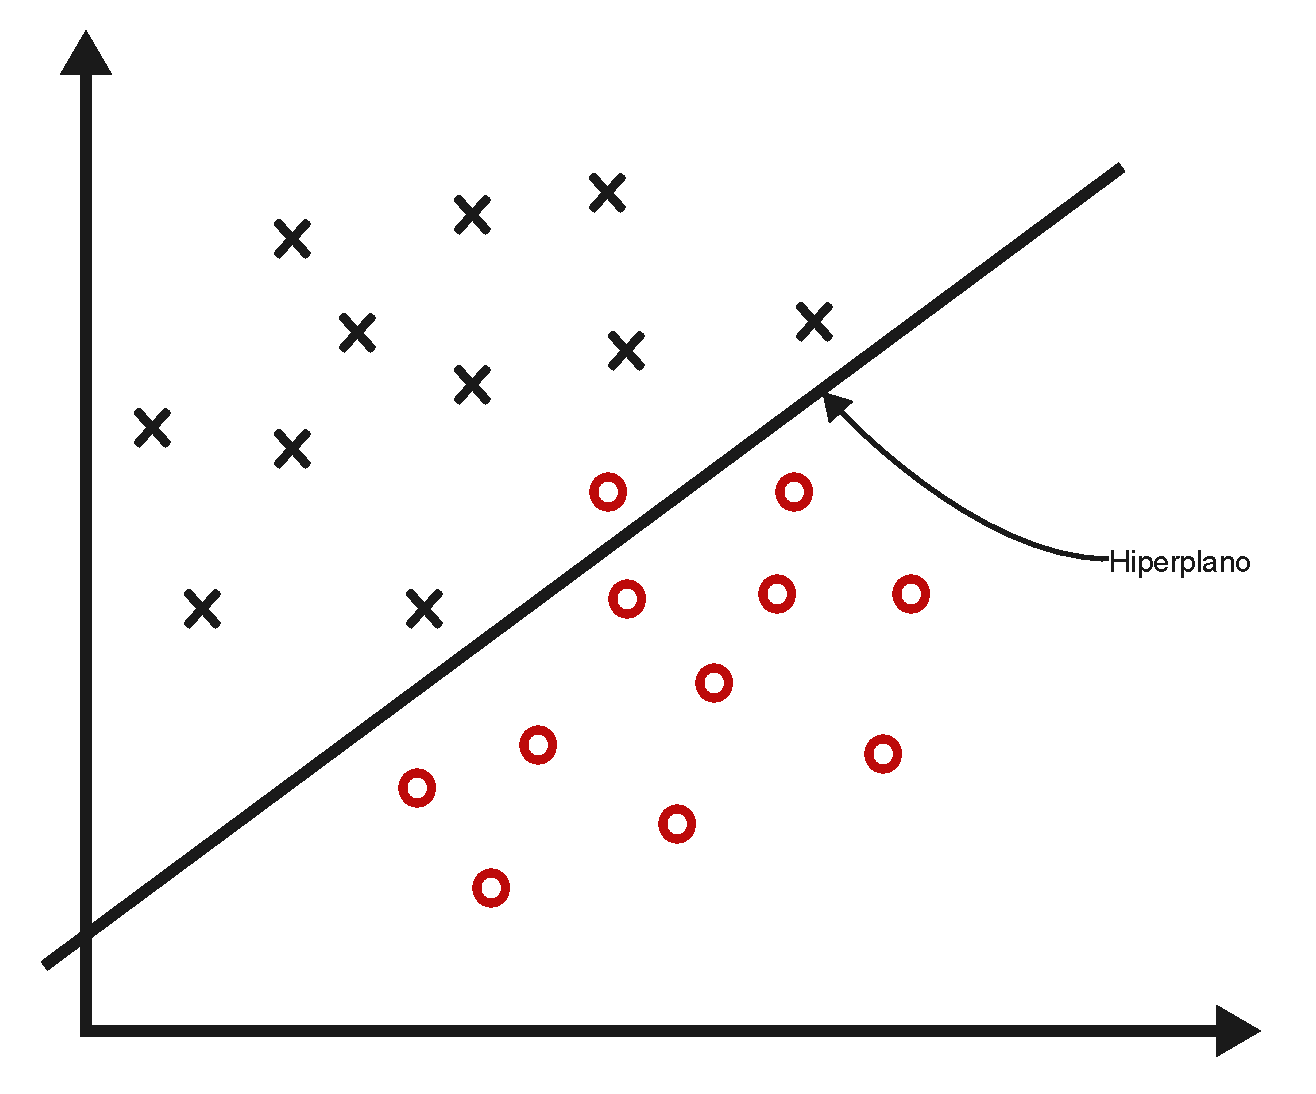
\includegraphics[width=0.6\textwidth]{images/hiperplano.pdf}
    \caption{Ejemplo bidimensional de un hiperplano que separa dos clases linealmente separables: las cruces negras pertenecen a una clase y los círculos rojos a la otra.}
    \label{fig:hiperplano_clasificacion}
\end{figure}

\section{Redes neuronales feedforward}

\subsection{Capas densas y notación matricial}

Una \textbf{capa densa} (o \textit{fully-connected}) agrupa muchas neuronas en paralelo. Sea $x \in \R^{d_{\text{in}}}$ la entrada a la capa. Una capa densa con $d_{\text{out}}$ neuronas se define como:
\begin{equation}
    z = W x + b, \quad z \in \R^{d_{\text{out}}},
\end{equation}
\begin{equation}
    y = \phi(z),
\end{equation}
donde:
\begin{itemize}
    \item $W \in \R^{d_{\text{out}} \times d_{\text{in}}}$ es la matriz de pesos.
    \item $b \in \R^{d_{\text{out}}}$ es el vector de sesgo.
    \item $\phi$ se aplica componente a componente. ($\phi: \R^{d_{\text{out}}} \to \R^{d_{\text{out}}}$, donde $\phi(z)=(\phi(z_i))_i$)
\end{itemize}

Para un conjunto de $N$ ejemplos, se suele apilar las entradas en una matriz $X \in \R^{N \times d_{\text{in}}}$ y la salida en $Y \in \R^{N \times d_{\text{out}}}$.

\subsection{Composición de capas}

Una \textbf{red neuronal feedforward} (o \textit{Multilayer Perceptron}, MLP) consiste en la composición de varias capas de este tipo. Por ejemplo, con dos capas ocultas:
\begin{align}
    h_1 &= \phi_1(W_1 x + b_1), \\
    h_2 &= \phi_2(W_2 h_1 + b_2), \\
    \hat{y} &= W_3 h_2 + b_3, \qquad \hat{y} \in \R^{d_{\text{out}}},
\end{align}

donde:
\begin{itemize}
    \item $x$ es la entrada.
    \item $h_1, h_2$ son representaciones internas (\textit{features} aprendidas).
    \item $\hat{y}$ es la salida del modelo (por ejemplo, una predicción de la serie de tiempo).
\end{itemize}

Este esquema se generaliza a un número arbitrario de capas. La capacidad de aproximación universal de las redes neuronales feedforward (bajo condiciones suaves sobre las funciones de activación) asegura que, con suficiente ancho y profundidad, pueden aproximar funciones muy complejas.

\begin{figure}[H]
    \centering
    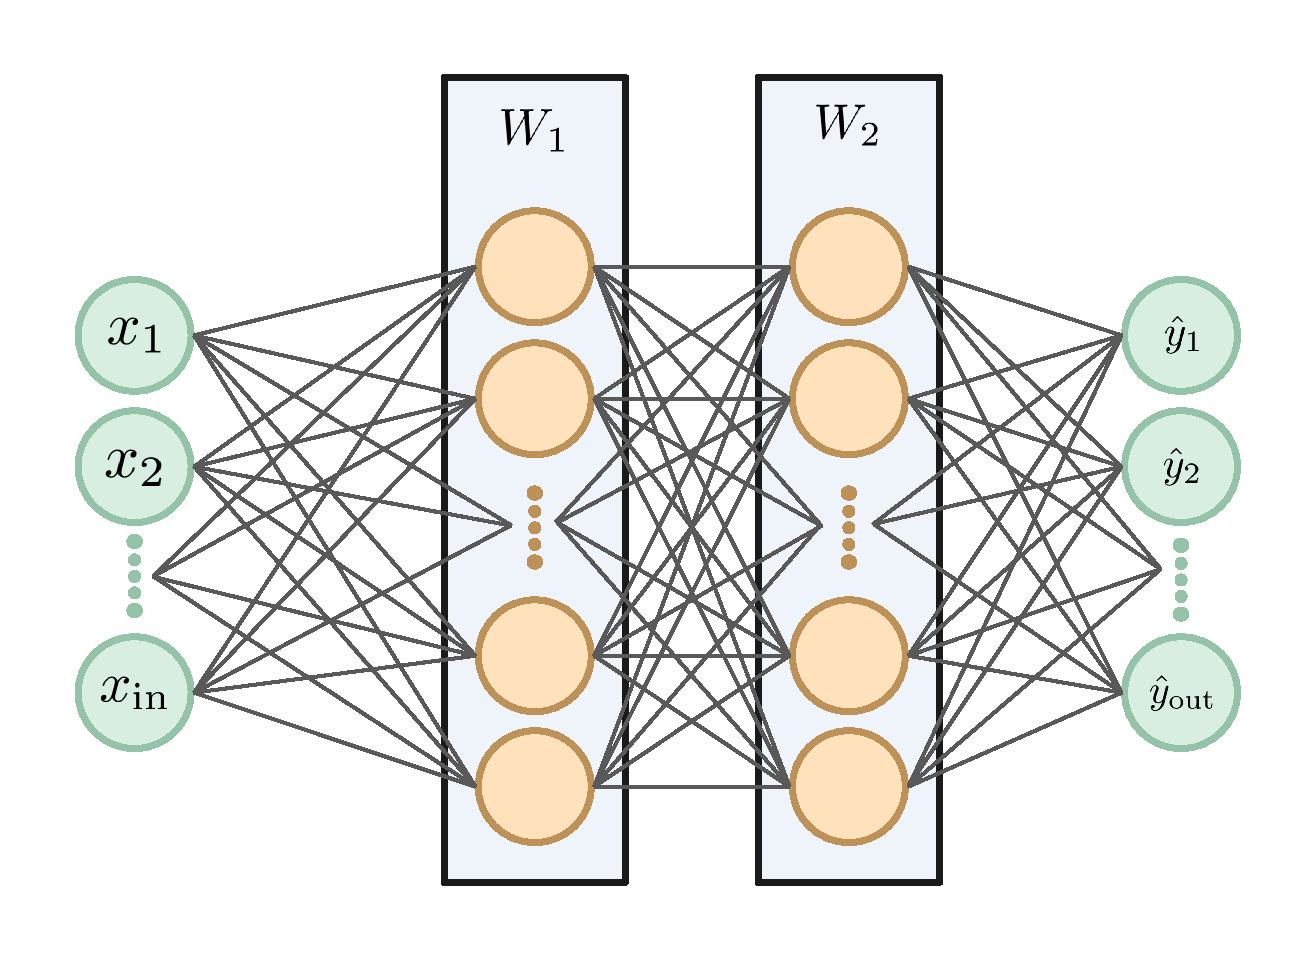
\includegraphics[width=0.6\textwidth]{images/Red neuronal.pdf}
    \caption{Esquema de una red neuronal \textit{feedforward} con dos capas ocultas: los vectores de entrada $x_1,\dots,x_{\text{in}}$ se transforman mediante las matrices de pesos $W_1$ y $W_2$ en representaciones internas, para finalmente producir las salidas $\hat{y}_1, \hat{y}_2, \dots, \hat{y}_{\text{out}}$.}
    \label{fig:red_mlp_dos_capas}
\end{figure}

\section{Función de pérdida}

\subsection{Pérdida para problemas de regresión}

En esta memoria el problema principal es de \textbf{regresión}: se quiere predecir un valor continuo (por ejemplo, el valor de una serie de tiempo en un instante futuro). Sea $\hat{y}_i$ la predicción del modelo para el ejemplo $i$ y $y_i$ el valor real. La función de pérdida más habitual es el \textbf{error cuadrático medio} (\textit{Mean Squared Error}, MSE):
\begin{equation}
    \mathcal{L}_{\text{MSE}}(\theta)
    = \frac{1}{N} \sum_{i=1}^{N} \|\hat{y}_i - y_i\|^2,
\end{equation}
donde $\theta$ representa el conjunto de todos los parámetros del modelo (todas las matrices $W$ y vectores $b$).

\hfill

El objetivo del entrenamiento es encontrar $\theta$ que minimice esta función de pérdida sobre el conjunto de datos de entrenamiento.

\hfill

Otras pérdidas útiles son, por ejemplo:
\begin{itemize}
    \item \textbf{Error absoluto medio} (MAE):
    \[
        \mathcal{L}_{\text{MAE}}(\theta)
        = \frac{1}{N} \sum_{i=1}^{N} \|\hat{y}_i - y_i\|_1.
    \]
    \item \textbf{Pérdida de Huber}, que combina propiedades de MSE y MAE, siendo más robusta a outliers.
\end{itemize}

\subsection{Regularización en la función de pérdida}

Para evitar sobreajuste (\textit{overfitting}), a menudo se agrega un término de \textbf{regularización} a la pérdida. Por ejemplo, regularización $L_2$ (también conocida como \textit{weight decay}):
\begin{equation}
    \mathcal{L}_{\text{total}}(\theta)
    = \mathcal{L}_{\text{datos}}(\theta)
    + \lambda \sum_{j} \|W_j\|_F^2,
\end{equation}
donde $\lambda > 0$ controla la fuerza de la regularización, y la suma recorre las matrices de pesos $W_j$ de cada capa.

\section{Descenso de gradiente y retropropagación}

\subsection{Descenso de gradiente}

El procedimiento básico para ajustar los parámetros de la red consiste en aplicar \textbf{descenso de gradiente}. Dada una función de pérdida $\mathcal{L}(\theta)$, el descenso de gradiente estándar actualiza los parámetros según:
\begin{equation}
    \theta_{t+1} = \theta_t - \eta \, \nabla_{\theta} \mathcal{L}(\theta_t),
\end{equation}
donde:
\begin{itemize}
    \item $\theta_t$ es el vector de parámetros en el paso $t$.
    \item $\eta > 0$ es la tasa de aprendizaje (\textit{learning rate}).
    \item $\nabla_{\theta} \mathcal{L}(\theta_t)$ es el gradiente de la pérdida respecto de los parámetros.
\end{itemize}

En la práctica, los datasets suelen ser grandes, por lo que calcular el gradiente sobre todos los datos en cada paso es costoso. Por ello se utiliza \textbf{descenso de gradiente estocástico} (SGD) o variantes \textit{mini-batch}, en las que el gradiente se estima a partir de un subconjunto de ejemplos:
\begin{equation}
    \theta_{t+1} = \theta_t - \eta \, \nabla_{\theta} \mathcal{L}_\mathcal{B}(\theta_t),
\end{equation}
donde $\mathcal{B}$ es un mini-batch de índices de entrenamiento.

\subsection{Retropropagación (\textit{backpropagation})}

Para poder aplicar descenso de gradiente, se requiere calcular el gradiente de la pérdida respecto de todos los parámetros de la red. Esto se logra mediante el algoritmo de \textbf{retropropagación}, que se basa en la regla de la cadena del cálculo diferencial.

\hfill

A nivel conceptual, la red se puede ver como una composición de funciones:
\begin{equation}
    \hat{y} = f_L \circ f_{L-1} \circ \cdots \circ f_1(x; \theta),
\end{equation}
donde cada $f_\ell$ representa una capa y depende de un subconjunto de parámetros $\theta_\ell$.

La regla de la cadena indica que:
\begin{equation}
    \frac{\partial \mathcal{L}}{\partial \theta_\ell}
    = \frac{\partial \mathcal{L}}{\partial f_\ell} \cdot 
      \frac{\partial f_\ell}{\partial \theta_\ell},
\end{equation}
y que las derivadas $\frac{\partial \mathcal{L}}{\partial f_\ell}$ se pueden calcular recursivamente desde la salida hacia la entrada.

\hfill

En términos prácticos:
\begin{enumerate}
    \item \textbf{Paso forward:} se propaga la entrada a través de la red y se calcula la pérdida.
    \item \textbf{Paso backward:} se calcula el gradiente de la pérdida respecto de la salida y se va propagando hacia atrás, capa por capa, acumulando las derivadas parciales.
    \item \textbf{Actualización:} se actualizan los parámetros usando el gradiente calculado y el algoritmo de optimización elegido (SGD, Adam, etc.).
\end{enumerate}

En frameworks modernos como PyTorch, este proceso se implementa automáticamente mediante \textit{autograd}, siempre que las operaciones definidas en el modelo sean diferenciables.

\section{Funciones de activación}

\subsection{Requisitos básicos}

La función de activación $\phi$ cumple dos roles fundamentales:
\begin{itemize}
    \item Introducir \textbf{no linealidad}. Sin funciones de activación, la composición de capas lineales sigue siendo una transformación lineal global.
    \item Ser \textbf{diferenciable} (al menos por tramos) para poder aplicar retropropagación.
\end{itemize}

A continuación se describen algunas de las funciones de activación más utilizadas.

\subsection{Sigmoide y tangente hiperbólica}

La función \textbf{sigmoide} se define como:
\begin{equation}
    \sigma(z) = \frac{1}{1 + e^{-z}}.
\end{equation}
Sus valores están en el intervalo $(0, 1)$ y su derivada es:
\begin{equation}
    \sigma'(z) = \sigma(z) \, (1 - \sigma(z)).
\end{equation}

La \textbf{tangente hiperbólica} se define como:
\begin{equation}
    \tanh(z) = \frac{e^{z} - e^{-z}}{e^{z} + e^{-z}},
\end{equation}
con valores en $(-1, 1)$ y derivada:
\begin{equation}
    \tanh'(z) = 1 - \tanh^2(z).
\end{equation}

Ambas funciones se usaron ampliamente en redes neuronales clásicas, pero presentan el problema de \textbf{gradientes que se desvanecen} (\textit{vanishing gradients}) para valores de $|z|$ grandes, lo que dificulta el entrenamiento de redes profundas.

\subsection{ReLU y variantes}

La \textbf{Rectified Linear Unit} (ReLU) se define como:
\begin{equation}
    \mathrm{ReLU}(z) = \max(0, z).
\end{equation}
Su derivada es:
\[
    \mathrm{ReLU}'(z) =
    \begin{cases}
        1, & z > 0, \\
        0, & z \le 0.
    \end{cases}
\]

Las ReLU han sido muy exitosas en redes profundas porque mitigan parcialmente el problema de gradientes que se desvanecen en la región $z > 0$ y son computacionalmente simples. Sin embargo, pueden producir neuronas ``muertas'' (salida cero constante) si los pesos se actualizan de forma que $z$ permanezca en la región negativa.

\hfill

Variantes como \textbf{Leaky ReLU} introducen un pequeño gradiente en la región negativa:
\[
    \mathrm{LeakyReLU}(z) =
    \begin{cases}
        z, & z > 0, \\
        \alpha z, & z \le 0,
    \end{cases}
\]
con $\alpha$ pequeño (por ejemplo, $\alpha = 0{,}01$).

\hfill

En modelos más recientes, incluyendo Transformers, es frecuente usar activaciones más suaves como \textbf{GELU} (\textit{Gaussian Error Linear Unit}), que puede verse como una versión suavizada de ReLU con ciertas propiedades teóricas favorables.

\section{Problemas en el entrenamiento de redes profundas}

\subsection{Gradientes que se desvanecen y explotan}

En redes profundas, al aplicar retropropagación, se multiplican muchas matrices y derivadas de funciones de activación. Esto puede llevar a que:
\begin{itemize}
    \item Los gradientes se hagan extremadamente pequeños (\textbf{vanishing gradients}), dificultando el aprendizaje en capas tempranas.
    \item Los gradientes crezcan de forma descontrolada (\textbf{exploding gradients}), causando inestabilidad numérica.
\end{itemize}

Existen varias estrategias para mitigar estos problemas:
\begin{itemize}
    \item Diseñar buenas \textbf{inicializaciones} de los pesos (por ejemplo, He o Xavier).
    \item Utilizar funciones de activación adecuadas (ReLU, GELU, etc.).
    \item Aplicar \textbf{normalizaciones}, como \textit{Batch Normalization} o \textit{Layer Normalization}.
    \item Aplicar \textbf{clipping de gradiente}, limitando la norma del gradiente en cada actualización.
\end{itemize}

\subsection{Regularización y generalización}

Además de los términos de regularización en la pérdida, existen técnicas adicionales para mejorar la capacidad de generalización:
\begin{itemize}
    \item \textbf{Dropout}: durante el entrenamiento, se anulan aleatoriamente algunas neuronas (se ponen a cero) con cierta probabilidad, lo que fuerza al modelo a no depender excesivamente de un subconjunto pequeño de unidades.
    \item \textbf{Early stopping}: se detiene el entrenamiento cuando la pérdida de validación deja de mejorar, evitando sobreajuste.
    \item \textbf{Data augmentation}: en dominios como imágenes o texto, se generan ejemplos adicionales modificando ligeramente los datos originales. En series de tiempo esto es más delicado, pero existen técnicas específicas.
\end{itemize}

\section{Optimizadores avanzados: Adam}

\subsection{Motivación}

El descenso de gradiente estándar utiliza una única tasa de aprendizaje $\eta$ para todos los parámetros y no tiene memoria explícita del historial de gradientes. En problemas complejos y de alta dimensión, esto puede hacer que:
\begin{itemize}
    \item El entrenamiento sea sensible a la elección de $\eta$.
    \item El modelo tarde en converger o quede atrapado en regiones poco favorables.
\end{itemize}

Por ello se han desarrollado \textbf{optimizadores avanzados} que adaptan la tasa de aprendizaje de manera automática, utilizando información adicional sobre la historia del gradiente. Uno de los más usados en la práctica es \textbf{Adam} (\textit{Adaptive Moment Estimation}).

\subsection{Algoritmo Adam}

Sea $\theta_t$ el vector de parámetros en el paso $t$ y $g_t = \nabla_\theta \mathcal{L}_t(\theta_t)$ el gradiente de la pérdida calculado en ese paso (por ejemplo, sobre un mini-batch). Adam mantiene dos variables auxiliares:
\begin{itemize}
    \item $m_t$: estimación del primer momento (media) del gradiente.
    \item $v_t$: estimación del segundo momento (varianza no centrada) del gradiente.
\end{itemize}

El algoritmo puede describirse como sigue:

\begin{enumerate}
    \item Inicializar $m_0 = 0$, $v_0 = 0$, $t = 0$.
    \item En cada paso:
    \begin{align}
        t &\leftarrow t + 1, \\
        g_t &\leftarrow \nabla_\theta \mathcal{L}_t(\theta_t), \\
        m_t &\leftarrow \beta_1 m_{t-1} + (1 - \beta_1) g_t, \\
        v_t &\leftarrow \beta_2 v_{t-1} + (1 - \beta_2) g_t^2,
    \end{align}
    donde las operaciones son componente a componente y $0 < \beta_1, \beta_2 < 1$ son hiperparámetros (típicamente $\beta_1 \approx 0{,}9$, $\beta_2 \approx 0{,}999$).
    \item Para corregir el sesgo inicial (ya que $m_t$ y $v_t$ parten en cero), se calculan:
    \begin{align}
        \hat{m}_t &= \frac{m_t}{1 - \beta_1^{t}}, \\
        \hat{v}_t &= \frac{v_t}{1 - \beta_2^{t}}.
    \end{align}
    \item Finalmente, se actualizan los parámetros:
    \begin{equation}
        \theta_{t+1}
        = \theta_t - \eta \, \frac{\hat{m}_t}{\sqrt{\hat{v}_t} + \varepsilon},
    \end{equation}
    donde $\eta$ es la tasa de aprendizaje base y $\varepsilon$ es un pequeño valor positivo (por ejemplo, $10^{-8}$) para evitar divisiones por cero.
\end{enumerate}

En palabras simples:
\begin{itemize}
    \item $m_t$ actúa como un \textbf{promedio móvil} del gradiente (similar a \textit{momentum}).
    \item $v_t$ actúa como un promedio móvil de la magnitud cuadrática del gradiente, permitiendo \textbf{adaptar} la escala de los pasos por parámetro.
    \item La división por $\sqrt{\hat{v}_t}$ hace que los parámetros con gradientes consistentemente grandes tengan pasos de actualización más pequeños, y viceversa.
\end{itemize}

En esta memoria se utiliza AdamW como optimizador principal para entrenar los modelos Transformer, tal como se especifica en los archivos de configuración de entrenamiento. AdamW conserva el carácter adaptativo de Adam, pero desacopla el decaimiento de pesos de la actualización basada en momentos.

\section{Relación con \CTTransformer}

Aunque el Transformer parece, a primera vista, una arquitectura muy distinta a un MLP estándar, en el fondo reutiliza los mismos componentes básicos descritos en este anexo:

\begin{itemize}
    \item Cada bloque de \textbf{atención multi-cabeza} está compuesto por proyecciones lineales (capas densas) que calculan las matrices de \textit{queries}, \textit{keys} y \textit{values}, seguidas de operaciones de atención y una proyección lineal de salida.
    \item El \textbf{bloque feed-forward} dentro de cada capa del Transformer es esencialmente un MLP de dos capas aplicado posición a posición, con una función de activación no lineal (por ejemplo, ReLU o GELU).
    \item La red completa se entrena minimizando una función de pérdida (en este caso, típicamente MSE sobre las predicciones de la serie de tiempo) usando descenso de gradiente y un optimizador como Adam o AdamW.
    \item La \textbf{cabeza de regresión} sobre el token \textit{target} en el modelo de esta memoria es, nuevamente, una capa lineal (o una pequeña MLP) que transforma la representación latente del token en la predicción final.
\end{itemize}

Por lo tanto, comprender el funcionamiento de neuronas, funciones de activación, retropropagación y optimizadores adaptativos como Adam o AdamW es suficiente para entender el entrenamiento de toda la arquitectura \CTTransformer, aunque los detalles de la atención, los encodings temporales y el scheduler usado en los experimentos se desarrollen en capítulos específicos y en el Anexo~\ref{anexo:optimizacion-scheduler}.

\section{Resumen del anexo}

En este anexo se han presentado los fundamentos necesarios para comprender el entrenamiento de redes neuronales modernas:
\begin{itemize}
    \item El modelo de neurona artificial como combinación lineal más función de activación.
    \item La construcción de redes feedforward mediante la composición de capas densas.
    \item La definición de funciones de pérdida para problemas de regresión y el uso de regularización.
    \item El algoritmo de entrenamiento basado en descenso de gradiente, estimado mediante mini-batches, y el cálculo eficiente de gradientes mediante retropropagación.
    \item El rol de las funciones de activación y los problemas asociados al entrenamiento de redes profundas (gradientes que se desvanecen o explotan).
    \item El algoritmo Adam y su variante AdamW como optimizadores adaptativos ampliamente utilizados en la práctica.
\end{itemize}

Estos conceptos constituyen la base sobre la cual se construyen las arquitecturas específicas analizadas en la memoria, en particular \CTTransformer.

\chapter{Detalles de optimización y scheduler}
\label{anexo:optimizacion-scheduler}

Este anexo complementa la descripción general de optimización presentada en el Anexo~\ref{anexo:fundamentos-redes}. Ambos protocolos usan AdamW, pero no el mismo scheduler: el benchmark legado emplea calentamiento lineal seguido de decaimiento coseno; la evaluación física congelada emplea \textttbreak{CosineAnnealingLR} sin calentamiento.

\section{AdamW}
\label{anexo:adamw}

Adam estima momentos de primer y segundo orden del gradiente para adaptar la escala de actualización de cada parámetro \cite{kingma2015adam}. En la práctica, para modelos Transformer se usa frecuentemente AdamW, que separa la regularización por decaimiento de pesos de la actualización adaptativa \cite{loshchilov2019decoupled}. Esta separación evita mezclar el término de regularización con los momentos acumulados del gradiente.

Si $\theta_t$ representa los parámetros, $\eta_t$ la tasa de aprendizaje de la época o paso actual, y $m_t$, $v_t$ los momentos corregidos por sesgo, AdamW puede verse esquemáticamente como:
\begin{equation}
    \theta_{t+1}
    =
    \theta_t
    -
    \eta_t
    \left(
        \frac{\hat{m}_t}{\sqrt{\hat{v}_t}+\varepsilon}
        +
        \lambda \theta_t
    \right),
\end{equation}
donde $\lambda$ controla el decaimiento de pesos. La idea importante para esta memoria es que $\eta_t$ no se mantiene constante: se modifica durante el entrenamiento mediante un scheduler.

\section{Benchmark legado: calentamiento lineal y decaimiento coseno}
\label{anexo:warmup-cosine}

En el benchmark legado no se usa un CosineAnnealingLR puro, sino una variante con \textbf{calentamiento lineal} (\emph{linear warmup}) seguido de \textbf{decaimiento coseno}. El calentamiento lineal evita comenzar el entrenamiento con una tasa de aprendizaje demasiado alta cuando los pesos todavía no han estabilizado sus representaciones internas. Esta práctica es especialmente útil en arquitecturas Transformer, donde las capas de atención, normalización y proyecciones lineales pueden ser sensibles a los primeros pasos de optimización.

Sea $\eta_{\max}$ la tasa de aprendizaje base, $E$ el número máximo de épocas, $w$ el número de épocas de calentamiento y $e$ la época actual, indexada desde $0$. La tasa de aprendizaje efectiva se define como:
\begin{equation}
    \eta(e)
    =
    \eta_{\max} \cdot s(e),
\end{equation}
donde
\begin{equation}
    s(e)
    =
    \begin{cases}
        \dfrac{e+1}{w}, & e < w, \\[8pt]
        \dfrac{1}{2}
        \left[
            1 + \cos\left(
                \pi
                \dfrac{e-w}{E-w}
            \right)
        \right],
        & e \geq w.
    \end{cases}
\end{equation}
La primera rama aumenta la tasa de aprendizaje de forma aproximadamente lineal hasta $\eta_{\max}$. La segunda rama aplica un decaimiento suave con forma coseno, relacionado con la familia de políticas de \emph{cosine annealing} \cite{loshchilov2017sgdr}, hasta acercarse a cero al final del entrenamiento.

En la implementación, el scheduler se actualiza una vez por época. Para modelos pequeños y medianos se utiliza $E=30$ con $w=2$, para modelos grandes se utiliza $E=60$ con $w=5$. En variantes más inestables se mantiene la misma forma funcional, pero se aumenta el calentamiento mínimo a cinco épocas y se reduce la tasa de aprendizaje base.

\section{Evaluación física: CosineAnnealingLR sin warmup}
\label{anexo:diferencia-cosine}

CosineAnnealingLR corresponde al decaimiento coseno sin etapa inicial de calentamiento. La evaluación física congelada usa esta política directamente. En cambio, la configuración legada usa la política compuesta:
\[
    \text{linear warmup}
    \quad \longrightarrow \quad
    \text{cosine decay}.
\]
Por lo tanto, ``coseno'' no debe interpretarse de forma única en esta memoria: \emph{warmup + cosine decay} identifica la receta legada, mientras \textttbreak{CosineAnnealingLR} identifica la receta física sin warmup. Esta distinción forma parte de la configuración versionada y evita atribuir al modelo diferencias debidas al optimizador.

\include{documents/anexoC_detalles_implementacion}
\include{documents/anexoD_material_extra}

\end{document}
